% Options for packages loaded elsewhere
\PassOptionsToPackage{unicode}{hyperref}
\PassOptionsToPackage{hyphens}{url}
%
\documentclass[
  graybox,natbib,nospthms]{svmono}
\usepackage{amsmath,amssymb}
\usepackage{iftex}
\ifPDFTeX
  \usepackage[T1]{fontenc}
  \usepackage[utf8]{inputenc}
  \usepackage{textcomp} % provide euro and other symbols
\else % if luatex or xetex
  \usepackage{unicode-math} % this also loads fontspec
  \defaultfontfeatures{Scale=MatchLowercase}
  \defaultfontfeatures[\rmfamily]{Ligatures=TeX,Scale=1}
\fi
\usepackage{lmodern}
\ifPDFTeX\else
  % xetex/luatex font selection
  \setmonofont[Scale=0.7]{Source Code Pro}
\fi
% Use upquote if available, for straight quotes in verbatim environments
\IfFileExists{upquote.sty}{\usepackage{upquote}}{}
\IfFileExists{microtype.sty}{% use microtype if available
  \usepackage[]{microtype}
  \UseMicrotypeSet[protrusion]{basicmath} % disable protrusion for tt fonts
}{}
\makeatletter
\@ifundefined{KOMAClassName}{% if non-KOMA class
  \IfFileExists{parskip.sty}{%
    \usepackage{parskip}
  }{% else
    \setlength{\parindent}{0pt}
    \setlength{\parskip}{6pt plus 2pt minus 1pt}}
}{% if KOMA class
  \KOMAoptions{parskip=half}}
\makeatother
\usepackage{xcolor}
\usepackage[paperwidth=18.90cm, paperheight=24.58cm, top=2.1cm, bottom=2.1cm, inner=2cm, outer=2cm]{geometry}
\usepackage{color}
\usepackage{fancyvrb}
\newcommand{\VerbBar}{|}
\newcommand{\VERB}{\Verb[commandchars=\\\{\}]}
\DefineVerbatimEnvironment{Highlighting}{Verbatim}{commandchars=\\\{\}}
% Add ',fontsize=\small' for more characters per line
\usepackage{framed}
\definecolor{shadecolor}{RGB}{248,248,248}
\newenvironment{Shaded}{\begin{snugshade}}{\end{snugshade}}
\newcommand{\AlertTok}[1]{\textcolor[rgb]{0.33,0.33,0.33}{#1}}
\newcommand{\AnnotationTok}[1]{\textcolor[rgb]{0.37,0.37,0.37}{\textbf{\textit{#1}}}}
\newcommand{\AttributeTok}[1]{\textcolor[rgb]{0.27,0.27,0.27}{#1}}
\newcommand{\BaseNTok}[1]{\textcolor[rgb]{0.06,0.06,0.06}{#1}}
\newcommand{\BuiltInTok}[1]{#1}
\newcommand{\CharTok}[1]{\textcolor[rgb]{0.5,0.5,0.5}{#1}}
\newcommand{\CommentTok}[1]{\textcolor[rgb]{0.37,0.37,0.37}{\textit{#1}}}
\newcommand{\CommentVarTok}[1]{\textcolor[rgb]{0.37,0.37,0.37}{\textbf{\textit{#1}}}}
\newcommand{\ConstantTok}[1]{\textcolor[rgb]{0.37,0.37,0.37}{#1}}
\newcommand{\ControlFlowTok}[1]{\textcolor[rgb]{0.27,0.27,0.27}{\textbf{#1}}}
\newcommand{\DataTypeTok}[1]{\textcolor[rgb]{0.27,0.27,0.27}{#1}}
\newcommand{\DecValTok}[1]{\textcolor[rgb]{0.06,0.06,0.06}{#1}}
\newcommand{\DocumentationTok}[1]{\textcolor[rgb]{0.37,0.37,0.37}{\textbf{\textit{#1}}}}
\newcommand{\ErrorTok}[1]{\textcolor[rgb]{0.14,0.14,0.14}{\textbf{#1}}}
\newcommand{\ExtensionTok}[1]{#1}
\newcommand{\FloatTok}[1]{\textcolor[rgb]{0.06,0.06,0.06}{#1}}
\newcommand{\FunctionTok}[1]{\textcolor[rgb]{0.27,0.27,0.27}{\textbf{#1}}}
\newcommand{\ImportTok}[1]{#1}
\newcommand{\InformationTok}[1]{\textcolor[rgb]{0.37,0.37,0.37}{\textbf{\textit{#1}}}}
\newcommand{\KeywordTok}[1]{\textcolor[rgb]{0.27,0.27,0.27}{\textbf{#1}}}
\newcommand{\NormalTok}[1]{#1}
\newcommand{\OperatorTok}[1]{\textcolor[rgb]{0.43,0.43,0.43}{\textbf{#1}}}
\newcommand{\OtherTok}[1]{\textcolor[rgb]{0.37,0.37,0.37}{#1}}
\newcommand{\PreprocessorTok}[1]{\textcolor[rgb]{0.37,0.37,0.37}{\textit{#1}}}
\newcommand{\RegionMarkerTok}[1]{#1}
\newcommand{\SpecialCharTok}[1]{\textcolor[rgb]{0.43,0.43,0.43}{\textbf{#1}}}
\newcommand{\SpecialStringTok}[1]{\textcolor[rgb]{0.5,0.5,0.5}{#1}}
\newcommand{\StringTok}[1]{\textcolor[rgb]{0.5,0.5,0.5}{#1}}
\newcommand{\VariableTok}[1]{\textcolor[rgb]{0,0,0}{#1}}
\newcommand{\VerbatimStringTok}[1]{\textcolor[rgb]{0.5,0.5,0.5}{#1}}
\newcommand{\WarningTok}[1]{\textcolor[rgb]{0.37,0.37,0.37}{\textbf{\textit{#1}}}}
\usepackage{longtable,booktabs,array}
\usepackage{calc} % for calculating minipage widths
% Correct order of tables after \paragraph or \subparagraph
\usepackage{etoolbox}
\makeatletter
\patchcmd\longtable{\par}{\if@noskipsec\mbox{}\fi\par}{}{}
\makeatother
% Allow footnotes in longtable head/foot
\IfFileExists{footnotehyper.sty}{\usepackage{footnotehyper}}{\usepackage{footnote}}
\makesavenoteenv{longtable}
\usepackage{graphicx}
\makeatletter
\def\maxwidth{\ifdim\Gin@nat@width>\linewidth\linewidth\else\Gin@nat@width\fi}
\def\maxheight{\ifdim\Gin@nat@height>\textheight\textheight\else\Gin@nat@height\fi}
\makeatother
% Scale images if necessary, so that they will not overflow the page
% margins by default, and it is still possible to overwrite the defaults
% using explicit options in \includegraphics[width, height, ...]{}
\setkeys{Gin}{width=\maxwidth,height=\maxheight,keepaspectratio}
% Set default figure placement to htbp
\makeatletter
\def\fps@figure{htbp}
\makeatother
\setlength{\emergencystretch}{3em} % prevent overfull lines
\providecommand{\tightlist}{%
  \setlength{\itemsep}{0pt}\setlength{\parskip}{0pt}}
\setcounter{secnumdepth}{5}
\usepackage{amsmath} % if desired
\usepackage{unicode-math}
%\setmathfont{latinmodern-math.otf}
\usepackage{float}
\usepackage{color}
\usepackage{fancyvrb}
\usepackage{longtable}
\usepackage{booktabs}
\usepackage{graphicx}
\providecommand{\tightlist}{\setlength{\itemsep}{0pt}\setlength{\parskip}{0pt}}
\usepackage[hyphens]{url}
\usepackage{hyperref}
%\usepackage{fontspec}
%\setsansfont{Roboto}[
%  Path = fonts/Roboto/,
%  Extension = .ttf,
%  UprightFont = *-Regular,
%  %-- Upright --%
%  FontFace={ul}{n}{Font=*-Thin},
%  FontFace={l}{n}{Font=*-Light},
%  FontFace={m}{n}{Font=*-Regular},
%  FontFace={mb}{n}{Font=*-Medium},
%  FontFace={b}{n}{Font=*-Bold},
%  FontFace={eb}{n}{Font=*-Black},
%  % %-- Italic --%
%  FontFace={ul}{it}{Font=*-ThinItalic},
%  FontFace={l}{it}{Font=*-LightItalic},
%  FontFace={m}{it}{Font=*-Italic},
%  FontFace={mb}{it}{Font=*-MediumItalic},
%  FontFace={b}{it}{Font=*-BoldItalic},
%  FontFace={eb}{it}{Font=*-BlackItalic},
%]

% Place links in parens
\renewcommand{\href}[2]{#2 (\url{#1})}
% Use auto ref for internal links
\let\oldhyperlink=\hyperlink
\renewcommand{\hyperlink}[2]{\autoref{#1}}
\def\chapterautorefname{Chapter}
\def\sectionautorefname{Section}
\def\subsectionautorefname{Section}
\def\subsubsectionautorefname{Section}

\setlength{\emergencystretch}{3em}  % prevent overfull lines
\vbadness=10000 % suppress underfull \vbox
\hbadness=10000 % suppress underfull \vbox
\hfuzz=10pt

\usepackage{framed,color}
\definecolor{shadecolor}{RGB}{231,231,231}

\renewcommand{\textfraction}{0.05}
\renewcommand{\topfraction}{0.8}
\renewcommand{\bottomfraction}{0.8}
\renewcommand{\floatpagefraction}{0.75}

\renewenvironment{quote}{\begin{VF}}{\end{VF}}
\let\oldhref\href
\renewcommand{\href}[2]{#2\footnote{\url{#1}}}

\let\BeginKnitrBlock\begin \let\EndKnitrBlock\end

\ifxetex
  \usepackage{letltxmacro}
  \setlength{\XeTeXLinkMargin}{1pt}
  \LetLtxMacro\SavedIncludeGraphics\includegraphics
  \def\includegraphics#1#{% #1 catches optional stuff (star/opt. arg.)
    \IncludeGraphicsAux{#1}%
  }%
  \newcommand*{\IncludeGraphicsAux}[2]{%
    \XeTeXLinkBox{%
      \SavedIncludeGraphics#1{#2}%
    }%
  }%
\fi

\makeatletter
\newenvironment{kframe}{%
\medskip{}
\setlength{\fboxsep}{.8em}
 \def\at@end@of@kframe{}%
 \ifinner\ifhmode%
  \def\at@end@of@kframe{\end{minipage}}%
  \begin{minipage}{\columnwidth}%
 \fi\fi%
 \def\FrameCommand##1{\hskip\@totalleftmargin \hskip-\fboxsep
 \colorbox{shadecolor}{##1}\hskip-\fboxsep
     % There is no \\@totalrightmargin, so:
     \hskip-\linewidth \hskip-\@totalleftmargin \hskip\columnwidth}%
 \MakeFramed {\advance\hsize-\width
   \@totalleftmargin\z@ \linewidth\hsize
   \@setminipage}}%
 {\par\unskip\endMakeFramed%
 \at@end@of@kframe}
\makeatother

\makeatletter
\@ifundefined{Shaded}{
}{\renewenvironment{Shaded}{\begin{kframe}}{\end{kframe}}}
\makeatother

\newenvironment{rmdblock}[1]
  {
  % \begin{itemize}
  % \renewcommand{\labelitemi}{
  %   \raisebox{-.7\height}[0pt][0pt]{
  %     {\setkeys{Gin}{width=3em,keepaspectratio}\includegraphics{images/#1}}
  %   }
  % }
  % \setlength{\fboxsep}{10em}
  \begin{kframe}
  % \item
  }
  {
  \end{kframe}
  % \end{itemize}
  }
\newenvironment{rmdnote}
  {\begin{rmdblock}{note}}
  {\end{rmdblock}}
\newenvironment{rmdcaution}
  {\begin{rmdblock}{caution}}
  {\end{rmdblock}}
\newenvironment{rmdimportant}
  {\begin{rmdblock}{important}}
  {\end{rmdblock}}
\newenvironment{rmdtip}
  {\begin{rmdblock}{tip}}
  {\end{rmdblock}}
\newenvironment{rmdwarning}
  {\begin{rmdblock}{warning}}
  {\end{rmdblock}}

\usepackage{makeidx}
\makeindex
\ifLuaTeX
  \usepackage{selnolig}  % disable illegal ligatures
\fi
\usepackage[]{natbib}
\bibliographystyle{spbasic}
\IfFileExists{bookmark.sty}{\usepackage{bookmark}}{\usepackage{hyperref}}
\IfFileExists{xurl.sty}{\usepackage{xurl}}{} % add URL line breaks if available
\urlstyle{same}
\hypersetup{
  pdftitle={OpenLandMap Open Land Data services},
  pdfauthor={OpenGeoHub foundation, GILAB.rs and contributors},
  hidelinks,
  pdfcreator={LaTeX via pandoc}}

\title{OpenLandMap Open Land Data services}
\author{OpenGeoHub foundation, GILAB.rs and contributors}
\date{}

\begin{document}
\maketitle

%\cleardoublepage\newpage\thispagestyle{empty}\null
%\cleardoublepage\newpage\thispagestyle{empty}\null
%\cleardoublepage\newpage
\thispagestyle{empty}
\begin{center}
% \includegraphics{images/dedication.pdf}
\end{center}

\setlength{\abovedisplayskip}{-5pt}
\setlength{\abovedisplayshortskip}{-5pt}

{
\setcounter{tocdepth}{1}
\tableofcontents
}
\hypertarget{about}{%
\chapter{About}\label{about}}

\href{https://openlandmap.org/}{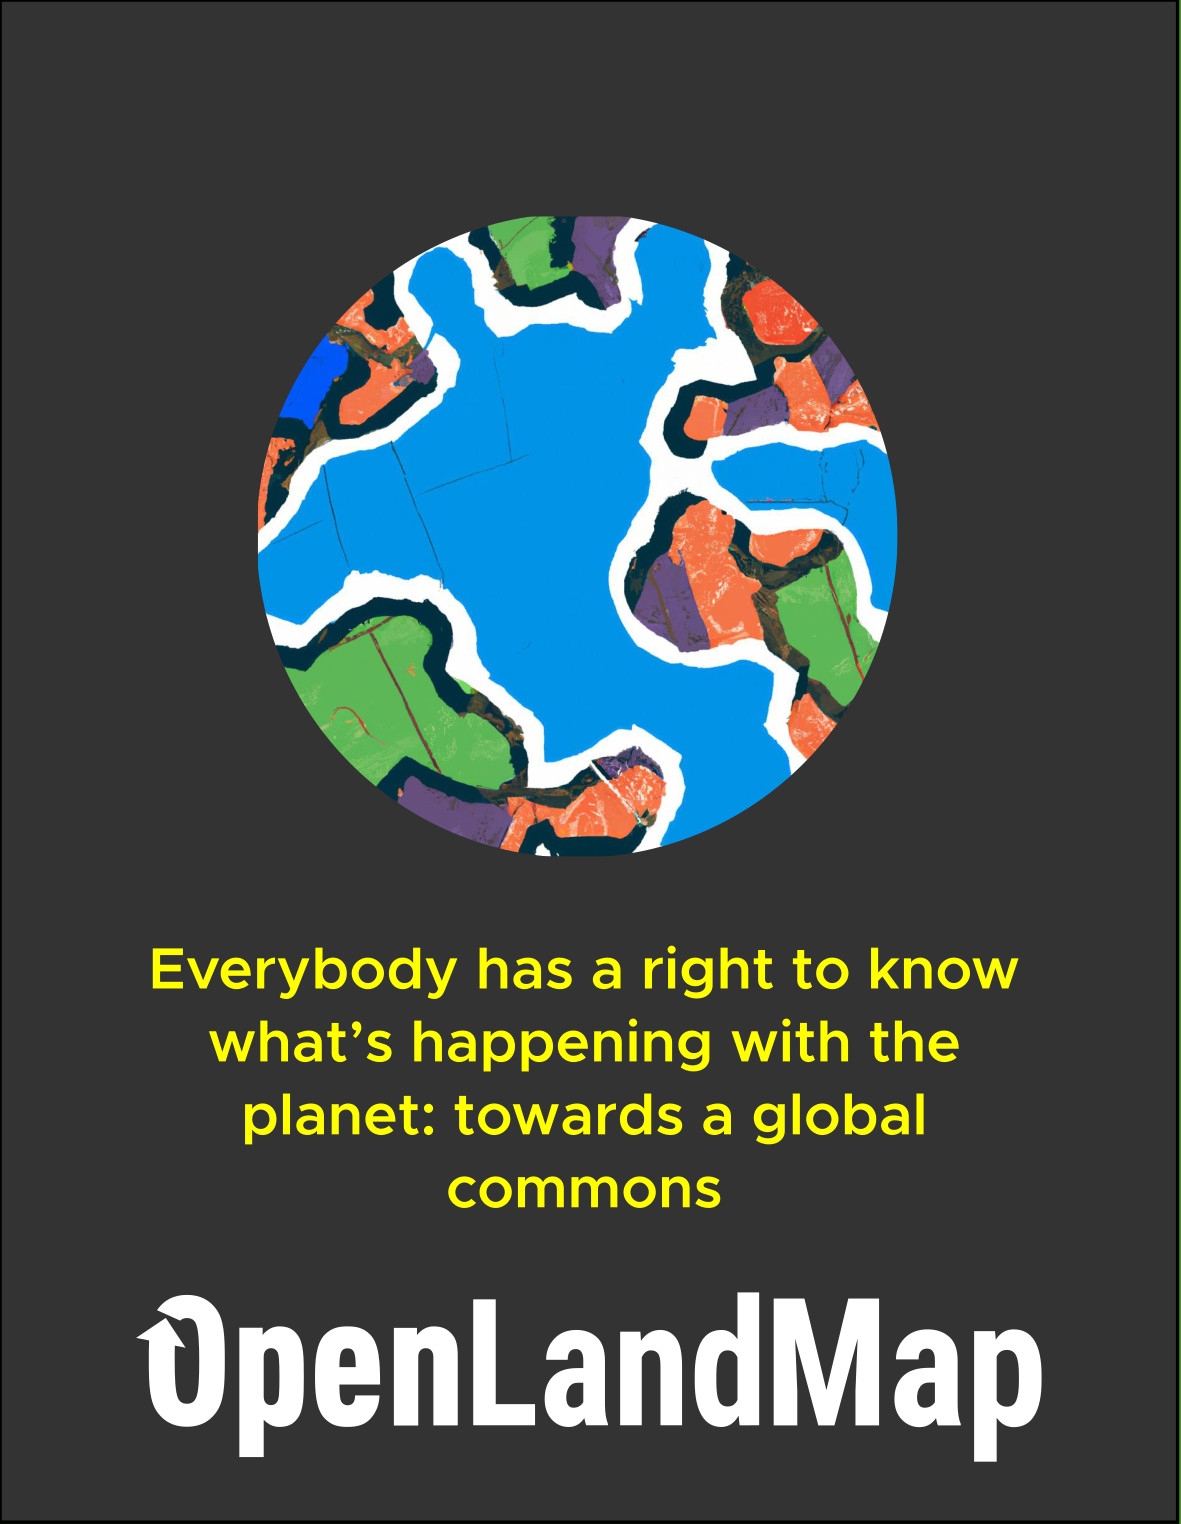
\includegraphics[width=2.60417in,height=\textheight]{cover.jpg}}

\href{https://doi.org/10.5281/zenodo.10466903}{
\includegraphics{zenodo.10466903_svg-tex.pdf}}

\hypertarget{openlandmap-project}{%
\section{OpenLandMap project}\label{openlandmap-project}}

\href{https://openlandmap.org}{OpenLandMap} are Open Land Data services providing access to spatial layers
covering global land mass (at spatial resolutions of 1-km, 250-m, 100-m, 30-m or finer) hosted by the OpenGeoHub foundation, GILAB.rs and collaborators.
It aims at becoming an \href{https://towardsdatascience.com/everybody-has-a-right-to-know-whats-happening-with-the-planet-towards-a-global-commons-5a1ad4ba0bdd}{OpenStreetMap-type system for land data}. Access to spatial layers is
possible via interactive visualizations and/or Open Source software solutions.
Read more about this project \href{https://opengeohub.org/about-openlandmap/}{here}.

The OpenLandMap layers, if not specified otherwise, are licensed under the
\href{https://creativecommons.org/licenses/by-sa/4.0/legalcode}{Creative Commons Attribution-ShareAlike 4.0 International license} (CC BY-SA) and/or
the \href{https://opendatacommons.org/licenses/odbl/}{Open Data Commons Open Database License} (ODbL). This implies that anyone can use,
or build upon, the OpenLandMap data without restrictions.
See the \href{https://opengeohub.org/about-openlandmap/}{Copyright and License} page for more details.

\begin{figure}

{\centering 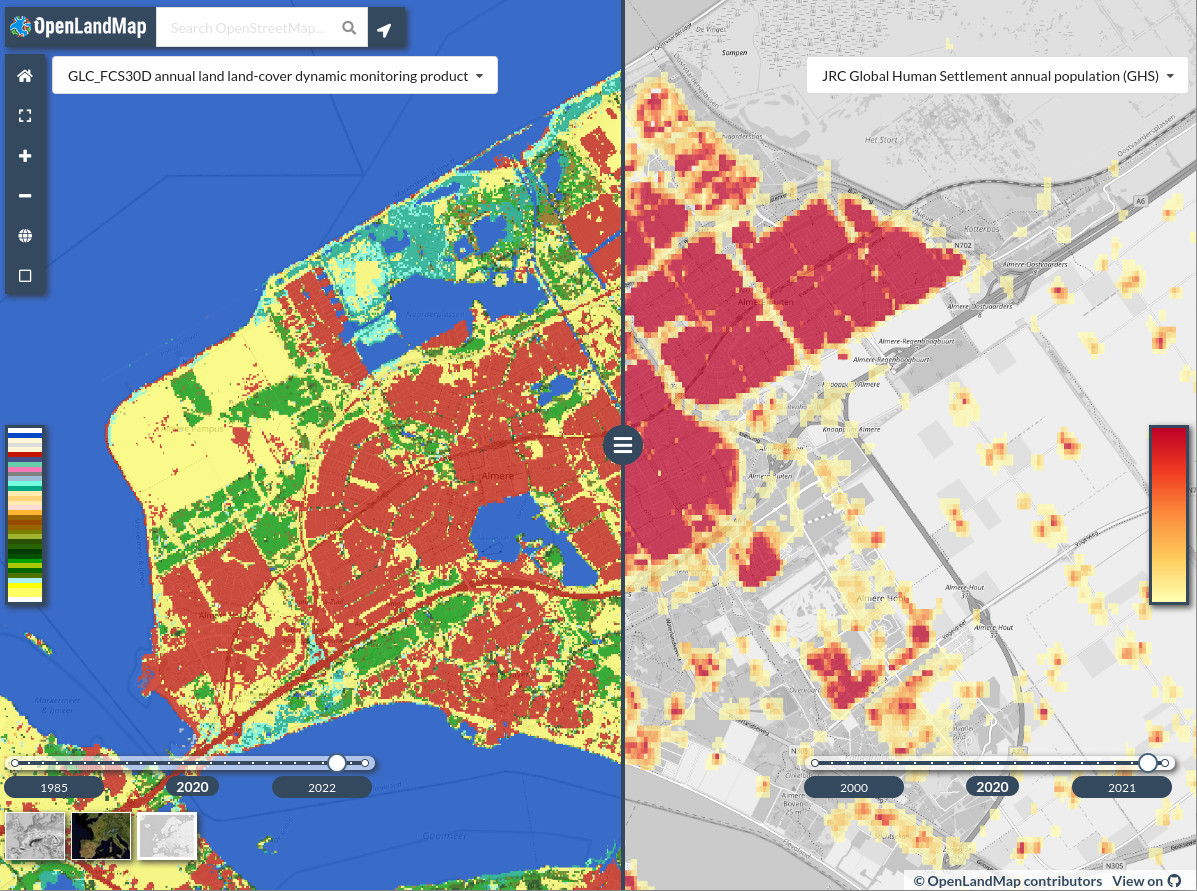
\includegraphics[width=1\linewidth]{img/openlandmap_gui_preview} 

}

\caption{Comparison tool in the OpenLandMap and time-sliders.}\label{fig:olm-istria}
\end{figure}

Users can access OpenLandMap data via the five main channels:

\begin{itemize}
\tightlist
\item
  \textbf{OpenLandMap App} at \url{https://openlandmap.org},
\item
  \textbf{OpenLandMap training points} at \url{https://github.com/openlandmap/compiled-ess-point-data-sets},
\item
  \textbf{OpenGeoHub STAC} installation at \url{https://stac.opengeohub.org},
\item
  \href{https://zenodo.org/search?page=1\&size=20\&q=OpenLandMap}{Zenodo.org} to access a (version-controlled) back-up copy of data via a DOI,
\end{itemize}

Data portal \url{https://openlandmap.org} is the landing page (running on Geoserver + OpenLayers) where users can browse maps, query values by
location, and find out about most recent news and activities. STAC at \url{https://stac.opengeohub.org}
is a generic layer repository for accessing layers installed and maintained by OpenGeoHub.
It allow users i.e.~producers of layers to edit and update metadata and descriptions,
create map views, learn how to use WCS, WMS or similar. A copy of the raw data can be obtained
via zenodo.org or similar public data repositories.

The \href{https://github.com/openlandmap/compiled-ess-point-data-sets}{training data repository} contains
import and processing steps run to clean up and standardize global compilations of training
points, most importantly the land cover, vegetation, meteo, soil and similar observations.

\hypertarget{layers-and-themes-of-interest}{%
\section{Layers and themes of interest}\label{layers-and-themes-of-interest}}

OpenLandMap.org provides access to global environmental layers focused on land surface.
We are aiming at serving Analysis-Ready, Cloud-Optimized (ARCO) data which passes \href{https://medium.com/mlearning-ai/present-and-future-of-data-cubes-an-european-eo-perspective-735d3f16f7c9}{four simple C checks} (4C):
(1) completeness (meaning: data is available for all or at least 99\% of pixels of interest),
(2) consistency (meaning: consistent file names, variable names and relationships,
and everything is documented via metadata), (3) currency (in this context: the user
is using the most up-to-date version of the data), (4) correctness (in this context:
making sure that the served data is the most correct / highest possible quality version).
In other words, ARCO version of the data should be something that is highest quality,
fully documented and optimized for web-services / advanced analysis.

Thus, the following five primary requirements need to be satisfied before a layer can be considered for inclusion:

\begin{itemize}
\tightlist
\item
  Global coverage with at least 98\% of the land mask represented in the layer (as not-NA values).
\item
  An \href{https://opendefinition.org/licenses/}{Open Data license}.
\item
  Metadata is supplied following the format specified below (all columns are filled-in and up-to-date).
\item
  Sufficient technical documentation is supplied --- usually as a scientific paper or a report.
\item
  A GDAL/proj4-compatible data format and projection system is used that allows for inclusion into Geoserver or similar.
\end{itemize}

All layers are organized around the following themes
(based on the \href{https://ggim.un.org/meetings/GGIM-committee/9th-Session/documents/Fundamental_Data_Publication.pdf}{UN-GGIM The Global Fundamental Geospatial Data Themes}):

\begin{itemize}
\tightlist
\item
  Buildings and Settlements,
\item
  Elevation and Depth,
\item
  Geology and Soils,
\item
  Land Cover and Land Use,
\item
  Population Distribution,
\item
  Water,
\item
  Physical Infrastructure,
\item
  Climate (\emph{added entry}),
\item
  Biodiversity and Nature Conservation (\emph{added entry}),
\end{itemize}

Note some layers maybe match two or more themes and are difficult to classify using a
simple definition, hence we might mention them at multiple places / within multiple themes.

\citet{RADELOFF2024113918} (the Landsat science team) have proposed 13 essential and
many more desirable/ aspirational products using medium resolution imagery referred
to as ``Medium-resolution satellite image-based products that meet the identified information needs for sustainable management, societal benefits, and global change challenges''.
The desirable products include: maps of crop types, irrigated fields, land abandonment,
forest loss agents, LAI/FAPAR, green vegetation cover fraction, emissivity, ice sheet
velocity, surface water quality and evaporative stress. The aspirational land monitoring
products include: forest types, and tree species, urban structure, forest recovery, crop yields,
forest biomass, habitat heterogeneity and winter habitat indices, net radiation,
snow and ice sheet surface melt, ice sheet and glacier melt ponds, sea ice motion and
evaporation and transpiration. This list is largely a basis for OpenLandMap activities for the years to come.

\hypertarget{accessing-data}{%
\section{Accessing data}\label{accessing-data}}

OpenLandMap data can be best accessed using the OpenLandMap \href{https://en.wikipedia.org/wiki/Amazon_S3}{S3} file service.
This service is based on \href{https://www.cogeo.org/}{Cloud-Optimized GeoTIFFs} and is
probably also the best solution for doing spatial queries and spatial analysis.

To connect and use data seamlessly in your code, we recommend using STAC tools e.g.~
\href{https://cran.r-project.org/web/packages/rstac/}{RStac} to access the OpenLanMap catalog
then program analysis by using the most up-to-date version of the data. You
can use the \url{https://s3.eu-central-1.wasabisys.com/stac/openlandmap/catalog.json} and
the \texttt{collection\_id} (example: \texttt{fapar\_essd.lstm}) to access description of data and
URLs of filenames on S3.

\hypertarget{accessing-data-from-zenodo}{%
\subsection{Accessing data from Zenodo}\label{accessing-data-from-zenodo}}

To download whole layers from zenodo you can use the R packages jsonlite and RCurl:

\begin{Shaded}
\begin{Highlighting}[]
\FunctionTok{library}\NormalTok{(jsonlite)}
\FunctionTok{library}\NormalTok{(RCurl)}
\FunctionTok{library}\NormalTok{(rgdal)}
\end{Highlighting}
\end{Shaded}

You first need to authenticate yourself by using a Zenodo API TOKEN
(see: \href{http://developers.zenodo.org/\#quickstart-upload}{how to obtain API TOKEN}):

\begin{Shaded}
\begin{Highlighting}[]
\NormalTok{TOKEN }\OtherTok{=} \FunctionTok{scan}\NormalTok{(}\StringTok{"\textasciitilde{}/TOKEN\_ACCESS"}\NormalTok{, }\AttributeTok{what=}\StringTok{"character"}\NormalTok{)}
\end{Highlighting}
\end{Shaded}

To download the \href{https://doi.org/10.5281/zenodo.1420114}{MODIS LST images at 1 km} you can use the bucket ID \texttt{dep.id\ =\ "1435938"} which gives:

\begin{Shaded}
\begin{Highlighting}[]
\NormalTok{dep.id }\OtherTok{=} \StringTok{"1435938"}
\NormalTok{x }\OtherTok{=} \FunctionTok{fromJSON}\NormalTok{(}\FunctionTok{system}\NormalTok{(}\FunctionTok{paste0}\NormalTok{(}\StringTok{\textquotesingle{}curl {-}H }\SpecialCharTok{\textbackslash{}"}\StringTok{Accept: application/json}\SpecialCharTok{\textbackslash{}"}\StringTok{ {-}H }\SpecialCharTok{\textbackslash{}"}\StringTok{Authorization: Bearer \textquotesingle{}}\NormalTok{, }
\NormalTok{        TOKEN, }\StringTok{\textquotesingle{}}\SpecialCharTok{\textbackslash{}"}\StringTok{ }\SpecialCharTok{\textbackslash{}"}\StringTok{https://zenodo.org/api/deposit/depositions/\textquotesingle{}}\NormalTok{, dep.id, }\StringTok{\textquotesingle{}}\SpecialCharTok{\textbackslash{}"}\StringTok{\textquotesingle{}}\NormalTok{), }\AttributeTok{intern=}\ConstantTok{TRUE}\NormalTok{))}
  \SpecialCharTok{\% Total    \%}\NormalTok{ Received \% Xferd  Average Speed   Time    Time     Time  Current}
\NormalTok{                                 Dload  Upload   Total   Spent    Left  Speed}
\DecValTok{100} \DecValTok{58704}  \DecValTok{100} \DecValTok{58704}    \DecValTok{0}     \DecValTok{0}  \DecValTok{80219}      \DecValTok{0} \SpecialCharTok{{-}{-}}\ErrorTok{:}\SpecialCharTok{{-}{-}}\ErrorTok{:}\SpecialCharTok{{-}{-}} \SpecialCharTok{{-}{-}}\ErrorTok{:}\SpecialCharTok{{-}{-}}\ErrorTok{:}\SpecialCharTok{{-}{-}} \SpecialCharTok{{-}{-}}\ErrorTok{:}\SpecialCharTok{{-}{-}}\ErrorTok{:}\SpecialCharTok{{-}{-}} \DecValTok{80196}
\end{Highlighting}
\end{Shaded}

\begin{verbatim}
  % Total    % Received % Xferd  Average Speed   Time    Time     Time  Current
                                 Dload  Upload   Total   Spent    Left  Speed
100 58704  100 58704    0     0  80219      0 --:--:-- --:--:-- --:--:-- 80196
> str(x, max.level = 1)
List of 15
 $ created     : chr "2018-09-26T18:37:50.432468+00:00"
 $ modified    : chr "2022-04-14T07:11:06.399928+00:00"
 $ id          : int 1435938
 $ conceptrecid: chr "1420114"
 $ doi         : chr "10.5281/zenodo.1435938"
 $ conceptdoi  : chr "10.5281/zenodo.1420114"
 $ doi_url     : chr "https://doi.org/10.5281/zenodo.1435938"
 $ metadata    :List of 15
 $ title       : chr "Long-term MODIS LST day-time and night-time temperatures, sd and differences at 1 km based on the 2000–2017 time series"
 $ links       :List of 21
 $ record_id   : int 1435938
 $ owner       : int 43652
 $ files       :'data.frame':   102 obs. of  5 variables:
 $ state       : chr "done"
 $ submitted   : logi TRUE
\end{verbatim}

This shows that there are total of 102 files in this folder. To download all temperatures for August,
we would hence use:

\begin{verbatim}
> sel.tif = x$files$links$download[grep("aug", x$files$links$download)]
\end{verbatim}

which gives a total of 9 files:

\begin{verbatim}
> sel.tif
[1] "https://zenodo.org/api/records/1435938/draft/files/clm_lst_mod11a2.aug.day_u.975_1km_s0..0cm_2000..2017_v1.0.tif/content"  
[2] "https://zenodo.org/api/records/1435938/draft/files/clm_lst_mod11a2.aug.day_l.025_1km_s0..0cm_2000..2017_v1.0.tif/content"  
[3] "https://zenodo.org/api/records/1435938/draft/files/clm_lst_mod11a2.aug.day_m_1km_s0..0cm_2000..2017_v1.0.tif/content"      
[4] "https://zenodo.org/api/records/1435938/draft/files/clm_lst_mod11a2.aug.daynight_m_1km_s0..0cm_2000..2017_v1.0.tif/content" 
[5] "https://zenodo.org/api/records/1435938/draft/files/clm_lst_mod11a2.aug.day_sd_1km.png/content"                             
[6] "https://zenodo.org/api/records/1435938/draft/files/clm_lst_mod11a2.aug.day_sd_1km_s0..0cm_2000..2017_v1.0.tif/content"     
[7] "https://zenodo.org/api/records/1435938/draft/files/clm_lst_mod11a2.aug.night_l.025_1km_s0..0cm_2000..2017_v1.0.tif/content"
[8] "https://zenodo.org/api/records/1435938/draft/files/clm_lst_mod11a2.aug.night_u.975_1km_s0..0cm_2000..2017_v1.0.tif/content"
[9] "https://zenodo.org/api/records/1435938/draft/files/clm_lst_mod11a2.aug.night_m_1km_s0..0cm_2000..2017_v1.0.tif/content" 
\end{verbatim}

We can test accessing the file by using:

\begin{verbatim}
tif = stringi::stri_replace_all_fixed(sel.tif[1], c("api/", "draft/", "/content"), "", vectorize_all=FALSE)
> system(paste0("gdalinfo /vsicurl/", tif))
Driver: GTiff/GeoTIFF
Files: /vsicurl/https://zenodo.org/records/1435938/files/clm_lst_mod11a2.aug.day_u.975_1km_s0..0cm_2000..2017_v1.0.tif
Size is 43200, 17924
Coordinate System is:
GEOGCRS["WGS 84",
    DATUM["World Geodetic System 1984",
        ELLIPSOID["WGS 84",6378137,298.257223563,
            LENGTHUNIT["metre",1]]],
    PRIMEM["Greenwich",0,
        ANGLEUNIT["degree",0.0174532925199433]],
    CS[ellipsoidal,2],
        AXIS["geodetic latitude (Lat)",north,
            ORDER[1],
            ANGLEUNIT["degree",0.0174532925199433]],
        AXIS["geodetic longitude (Lon)",east,
            ORDER[2],
            ANGLEUNIT["degree",0.0174532925199433]],
    ID["EPSG",4326]]
Data axis to CRS axis mapping: 2,1
Origin = (-180.000000000000000,87.370000000000005)
Pixel Size = (0.008333333333333,-0.008333333333333)
Metadata:
  AREA_OR_POINT=Area
Image Structure Metadata:
  COMPRESSION=DEFLATE
  INTERLEAVE=BAND
Corner Coordinates:
Upper Left  (-180.0000000,  87.3700000) (180d 0' 0.00"W, 87d22'12.00"N)
Lower Left  (-180.0000000, -61.9966667) (180d 0' 0.00"W, 61d59'48.00"S)
Upper Right ( 180.0000000,  87.3700000) (180d 0' 0.00"E, 87d22'12.00"N)
Lower Right ( 180.0000000, -61.9966667) (180d 0' 0.00"E, 61d59'48.00"S)
Center      (  -0.0000000,  12.6866667) (  0d 0' 0.00"W, 12d41'12.00"N)
Band 1 Block=43200x1 Type=Int16, ColorInterp=Gray
  NoData Value=-32767
  Overviews: 21600x8962, 10800x4481, 5400x2241, 2700x1121, 1350x561, 675x281, 338x141
\end{verbatim}

These files can be further downloaded using \texttt{download.file(tif,\ basename(tif))} function or similar.
There is also an R package for Zenodo \textbf{\href{https://github.com/eblondel/zen4R}{zen4R}}
that makes downloading files even easier. In python you can also the library
\textbf{\href{https://github.com/Open-Earth-Monitor/zen}{zen}} that is especially useful
for uploading very large data sets to Zenodo.

\hypertarget{accessing-data-from-google-earth-engine}{%
\subsection{Accessing data from Google Earth Engine}\label{accessing-data-from-google-earth-engine}}

\href{https://code.earthengine.google.com/?asset=users/opengeohub/openlandmap}{Google Earth Engine users} can access a snapshot of OpenLandMap.org layers using the following address:

\begin{itemize}
\tightlist
\item
  \url{https://code.earthengine.google.com/?asset=users/opengeohub/openlandmap}
\end{itemize}

Description of layer names and units used can be find \href{GEE/OpenLandMap_layers_for_GEE.pdf}{here}.
Note that sync between the layers on the OpenLandMap.org and Google Earth Engine is done
only once a year, hence, if you wish to use the most up-to-date layers at any moment,
downloading maps from either Zenodo or via the Wasabi service is recommended.

To access OpenLandMap layers you can also refer to the public data sets at:

\begin{itemize}
\tightlist
\item
  \url{https://developers.google.com/earth-engine/datasets/tags/openlandmap}
\end{itemize}

\hypertarget{the-file-naming-convention}{%
\section{The file naming convention}\label{the-file-naming-convention}}

The OpenLandMap file-naming convention works with 10 fields that basically define the most important properties of the data (this way users can search files, prepare data analysis etc, without even needing to access or open files. The 10 fields include:

\begin{enumerate}
\def\labelenumi{\arabic{enumi}.}
\tightlist
\item
  Generic variable name (needs to be unique): \texttt{lclu}
\item
  Variable procedure combination i.e.~method standard (standard abbreviation): \texttt{esa.cci}
\item
  Position in the probability distribution / variable type: \texttt{c}
\item
  Spatial support (usually horizontal block) in m or km: \texttt{250m}
\item
  Depth reference or depth interval e.g.~below (``b''), above (``a'') ground or at surface (``s'') b\{depth\}\{metric length\} for certain depth. e.g.~b30cm. For the interval we would like to go for b\{depth\}t\{depth\}\{metric length\}: \texttt{b30t60cm}
\item
  Time reference begin time (YYYYMMDD): \texttt{20210101}
\item
  Time reference end time: \texttt{20211231}
\item
  Bounding box (2 letters max): \texttt{go}
\item
  EPSG code: \texttt{epsg.4326}
\item
  Version code i.e.~creation date: \texttt{v20221015}
\end{enumerate}

An example of a file-name based on the description above:

\begin{verbatim}
lclu_esacci.lc.l4_c_250m_s_20210101_20211231_go_epsg.4326_v20221015.tif
\end{verbatim}

The following variable types are currently supported:

\begin{itemize}
\tightlist
\item
  \texttt{m}= mean value;
\item
  \texttt{q.10} = 10\% probability quantile (one side probability);
\item
  \texttt{d}= median value; equivalent to \texttt{q.50};
\item
  \texttt{c}= class or factor / requires a domain with codes / levels;
\item
  \texttt{cd} = change class (special cross-domain 2D matrix);
\item
  \texttt{p}= probability 0--100\%;
\item
  \texttt{sse} = Shannon Scaled Entropy index;
\item
  \texttt{l.159}= lower 68\% probability threshold (quantile);
\item
  \texttt{u.841}= upper 68\% probability threshold (quantile), for one-sided probability use ``\texttt{q}'',
\item
  \texttt{pc}= percent cover of the pixel 0--100\%;
\item
  \texttt{sd}= standard deviation or prediction error; for multiple standard deviation use e.g.~``\texttt{sd.2}''
\item
  \texttt{md} = model deviation (in the case of ensemble predictions);
\item
  \texttt{si}= confidence interval range for the prediction of the mean value;
\item
  \texttt{td} = cumulative difference (usually based on time-series of values);
\end{itemize}

Note that this file naming convention has the following properties:

\begin{itemize}
\tightlist
\item
  Large quantities of files can be easily sorted and searched (one line queries in Bash).
\item
  File-naming patterns can be used to seamlessly build virtual mosaics and composites.\\
\item
  Key spatiotemporal properties of the data are available in the file name e.g.~variable type, O\&M method, spatial resolution, bounding box, projection system, temporal references. Users can program analysis without opening or testing files.
\item
  Versioning system is ubiquitous.
\item
  All file-names are unique.
\end{itemize}

Geonetwork and STAC will be further used to link the unique file names to: (1) WPs, deliverables, themes / keywords, (2) DOI's, (3) project homepages, (4) contact pages for support and feedback. For keywords we recommend using the \href{https://inspire.ec.europa.eu/glossary}{INSPIRE keywords}. To confirm that metadata is complete and consistent, we recommend using the \href{https://inspire.ec.europa.eu/validator/home/index.html}{INSPIRE metadata validator} and/or \url{https://data.europa.eu/en} validator.

Some simple additional rules for generating the file name include:

\begin{enumerate}
\def\labelenumi{\arabic{enumi}.}
\tightlist
\item
  Codes and abbreviations should be human-readable as much as possible (hence short, but not too short!);
\item
  Use only English-US (en-us) language e.g.~for months use ``jan'', ``feb'' etc;
\item
  Consistently use \href{https://unicode.org/standard/standard.html}{UNICODE standard}: no non-ASCII characters;
\item
  Limit the total file name size in characters to: 256;
\item
  For time reference do not extend beyond hour minute and timezone;
\item
  For non-standard non-EPSG projections please register your projection first and obtain the code from \href{https://spatialreference.org/ref/epsg/}{Spatial Reference List};
\item
  For bounding boxes use as much as possible the 2--letter unique country code; for continents use the Equi7 Grid codes and for global products use ``go'' for global land without Antarctica, ``ga'' full global coverage,
\item
  For method codes use as much as possible unique IDs from \href{https://www.iso.org/standards-catalogue/browse-by-ics.html}{ISO - ICS};
\item
  For MODIS products use consistently the MODIS products codes e.g.~\href{https://lpdaac.usgs.gov/products/mod11a2v061/}{MOD11A2 v061};
\end{enumerate}

For long-term aggregates of seasonal, monthly, weekly values use the period name at the end of the method names (\#3) for example the long-term estimate of MODIS LST daytime temperature for month August:

\begin{verbatim}
lst.d_mod11a2v061.aug_m_1km_s_20200101_20211231_go_epsg.4326_v20221015.tif
\end{verbatim}

A list of vocabularies to be used as abbreviated names of variables will be provided by OpenGeoHub. The same file-name convention described above can be also used for vector data (this would only have a different file extension) also.

\hypertarget{the-land-mask}{%
\section{The land mask}\label{the-land-mask}}

The bounding box of interest for OpenLandMap data is:

\begin{verbatim}
Xmin = -180.00000
Ymin = -62.00081
Xmax = 179.99994
Ymax = 87.37000
\end{verbatim}

The image sizes at various standard resolutions are:

\begin{itemize}
\tightlist
\item
  250m = 172800P x 71698L,
\item
  500m = 86400P x 35849L,
\item
  1km = 43200P x 17924L,
\end{itemize}

\begin{figure}

{\centering 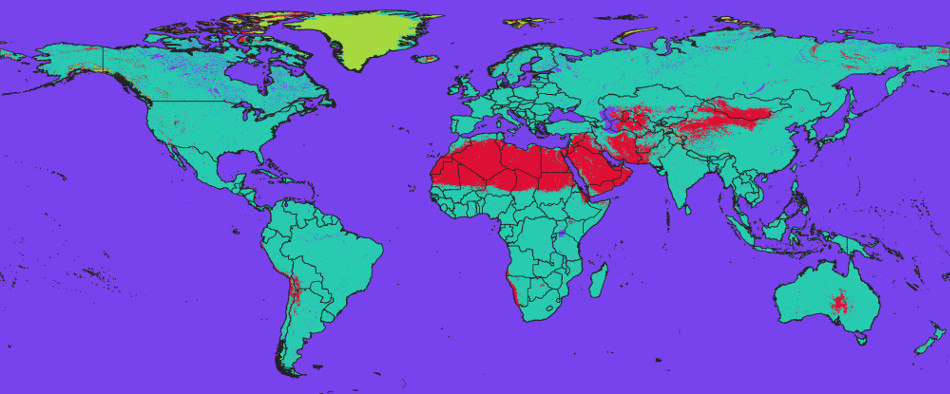
\includegraphics[width=1\linewidth]{img/landgis_world_mask} 

}

\caption{OpenLandMap world land mask: derived using the ESA land cover time series of maps 2000–2015. Red areas indicate barren lands, light green indicates permanent ice areas.}\label{fig:mask-word}
\end{figure}

The standard spatial resolutions are derived using simple
rule of thumb:

\begin{itemize}
\tightlist
\item
  250 m = 1/480 d.d. = 0.002083333
\item
  500 m = 1/240 d.d. = 0.004166667
\item
  1 km = 1/120 d.d. = 0.008333333
\end{itemize}

OpenLandMap works with a standard land mask derived using the \href{https://www.esa-landcover-cci.org/?q=node/175}{ESA time series of land cover maps 2000--2015}:

\begin{verbatim}
lcv_landmask_esacci.lc.l4_c_250m_s0..0cm_2000..2015_v1.0.tif
\end{verbatim}

📂 \href{https://doi.org/10.5281/zenodo.1476464}{Download layer}

It contains the following values:

\begin{itemize}
\item
  1 = land (all remaining pixels not permanent water, desert or ice)
\item
  2 = permanent water bodies (consistently water body 2000--2015)
\item
  3 = permanent bare areas (consistently bare areas /
  deserts 2000--2015)
\item
  4 = permanent ice (consistently ice 2000--2015)
\end{itemize}

If you need a global equal area projection (e.g.~to be able to derive total stocks / density of features in N/km-squared)
we advise using the \href{https://doi.org/10.5281/zenodo.3355006}{Goode Homolosine projection}:

\begin{verbatim}
+proj=igh +ellps=WGS84 +units=m +no_defs
\end{verbatim}

\begin{figure}

{\centering 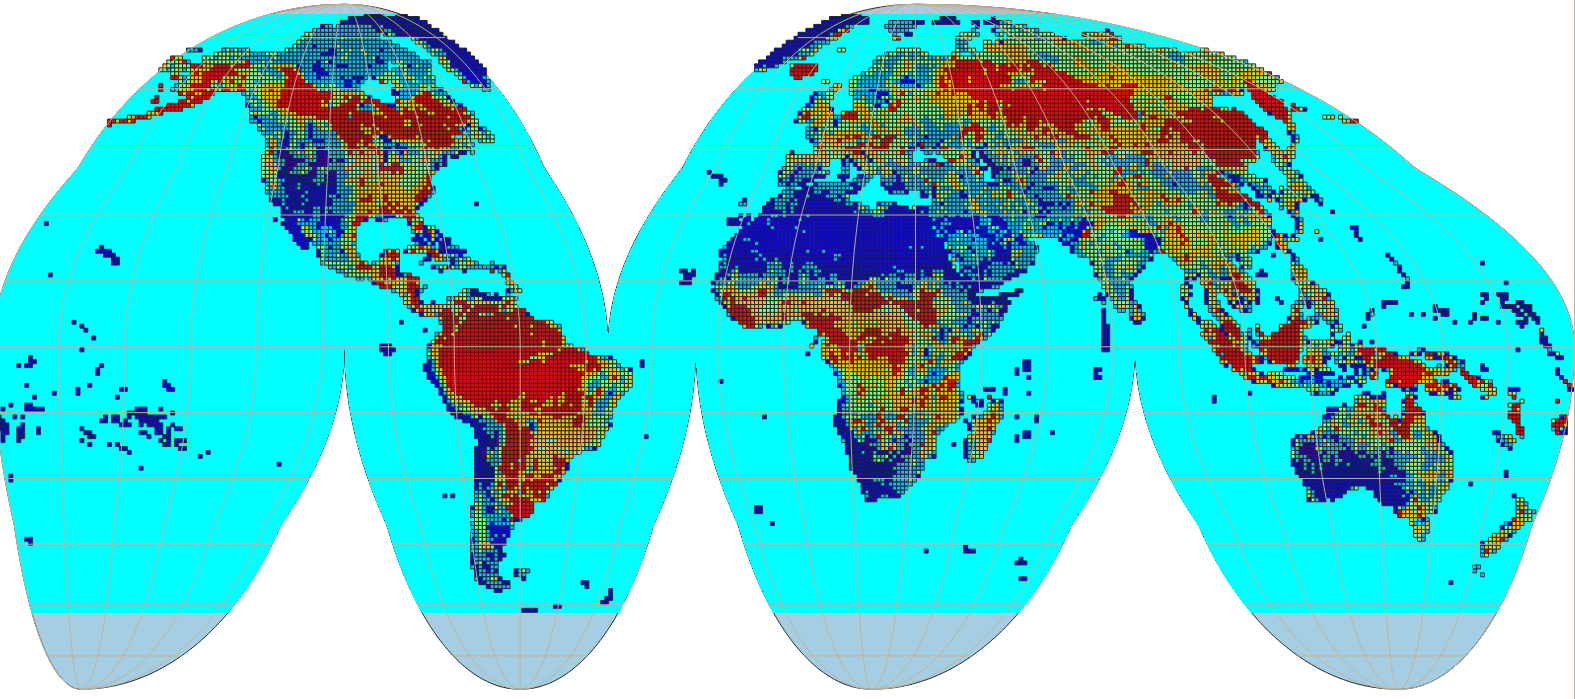
\includegraphics[width=1\linewidth]{img/001_preview_GH_100km_grid} 

}

\caption{OpenLandMap world mask in Goode Homolosine projection: 100 by 100 km blocks and land mask in the Goode Homolosine projection.}\label{fig:igh-world}
\end{figure}

📂 \href{https://doi.org/10.5281/zenodo.3355006}{Download layer}

The bounding box would in this case be:

\begin{verbatim}
Xmin = -20037508
Ymin = -6728980
Xmax = 20037508
Ymax = 8421750
\end{verbatim}

and the corresponding image sizes is:

\begin{itemize}
\tightlist
\item
  250m = 172800P x 71698L,
\end{itemize}

\hypertarget{cloud-optimized-geotiff}{%
\section{Cloud-optimized GeoTIFF}\label{cloud-optimized-geotiff}}

All layers included in the OpenLandMap system have been pre-processed following the GDAL's cloud-optimized GeoTIFF
instructions. To process large (global land mask at 250 m resolution or finer) GeoTIFFs please use the following
settings:

\begin{verbatim}
gdalwarp layer.vrt layer.tif 
   -ot COG
   -tr 0.002083333 0.002083333 
   -te -180.00000 -62.00081 179.99994 87.37000
   -wm 2000 -co \"BIGTIFF=YES\"
\end{verbatim}

To prepare a \href{https://trac.osgeo.org/gdal/wiki/CloudOptimizedGeoTIFF}{cloud-optimized GeoTIFF} use:

\begin{verbatim}
gdaladdo layer.tif -r near 2 4 8 16 32 64 128
gdal_translate layer.tif layer-co.tif -mo \"CO=YES\" -co \"TILED=YES\" -co \"BLOCKXSIZE=512\" 
        -co \"BLOCKYSIZE=512\" -co \"COMPRESS=LZW\" -co \"COPY_SRC_OVERVIEWS=YES\" 
        --config GDAL_TIFF_OVR_BLOCKSIZE 512
\end{verbatim}

This will add tiles and optimize compression. \texttt{CO=YES} indicates that the GeoTIFF has been cloud-optimized.

The OpenLandMap.org COG's are all available publicly without restrictions via the
\href{https://gitlab.com/openlandmap/global-layers/-/blob/master/tutorial/OpenLandMap_COG_tutorial.md}{Wasabi file service}.

\hypertarget{contributing-data}{%
\section*{Contributing data}\label{contributing-data}}
\addcontentsline{toc}{section}{Contributing data}

We encourage public and private entities to help this project and share SSL data.
The following four modes of data sharing are especially encouraged:

\begin{enumerate}
\def\labelenumi{\arabic{enumi}.}
\tightlist
\item
  Open your data by releasing it under Creative Commons (\href{https://creativecommons.org/licenses/by/4.0/}{CC-BY}, \href{https://creativecommons.org/licenses/by-sa/4.0/}{CC-BY-SA})\\
  or Open Data Commons Open Database License (\href{https://opendatacommons.org/licenses/odbl/}{ODbL}).
  This data can then directly imported into the OSSL.\\
\item
  Donate a small part (e.g.~5\%) of your data (release under \href{https://creativecommons.org/licenses/by/4.0/}{CC-BY}, \href{https://creativecommons.org/licenses/by-sa/4.0/}{CC-BY-SA} and/or \href{https://opendatacommons.org/licenses/odbl/}{ODbL}).
  This data can then directly imported into the OSSL.\\
\item
  Allow openlandmap.org project direct access to your data so that we can run data mining
  and then release ONLY results of data mining under some Open Data license.\\
\item
  Use OpenLandMap data to produce new derivative products, then share them through own
  infrastructures OR contact us for providing hosting support.
\end{enumerate}

We can sign professional \textbf{Data Sharing Agreements} with data producers
that specify in detail how will the data be used. Our primary interest is in enabling research,
sharing and use of models (calibration and prediction) and collaboration of groups
across borders.

We take especial care that your data is secured, encrypted where necessary,
and kept safely, closely following our \href{https://opengeohub.org/privacy-policy/}{privacy policy and terms of use}.

\hypertarget{contributing-documentation}{%
\section*{Contributing documentation}\label{contributing-documentation}}
\addcontentsline{toc}{section}{Contributing documentation}

Please feel free to contribute technical documentation. See \href{https://github.com/openlandmap/book}{GitHub
repository} for more detailed
instructions.

Information outdated or missing? Please \href{https://github.com/openlandmap/book/issues}{open an issue} or best do a
correction in the text and then make a \href{https://docs.github.com/en/github/collaborating-with-issues-and-pull-requests/creating-a-pull-request}{pull
request}.

\hypertarget{contributors}{%
\section*{Contributors}\label{contributors}}
\addcontentsline{toc}{section}{Contributors}

If you've contribute, add also your name and Twitter, ORCID or blog link
below:

\href{https://github.com/thengl}{Tomislav Hengl},
\href{https://www.linkedin.com/in/leal-parente/}{Leandro L. Parente},
\href{}{Rolf Simoes},

\hypertarget{disclaimer}{%
\section*{Disclaimer}\label{disclaimer}}
\addcontentsline{toc}{section}{Disclaimer}

Whilst utmost care has been taken by the Soil Spectroscopy project and data authors while
collecting and compiling the data, the data is provided \emph{``as is''}. \href{https://opengeohub.org/about}{OpenGeoHub foundation} and its
suppliers and licensors hereby disclaim all warranties of any kind, express or implied,
including, without limitation, the warranties of merchantability, fitness for a particular
purpose and non-infringement. Neither \href{https://opengeohub.org/about}{OpenGeoHub foundation} nor its suppliers and licensors,
makes any warranty that the Website will be error free or that access thereto will be
continuous or uninterrupted. You understand that you download from, or otherwise obtain
content or services through, the Website at your own discretion and risk.

In no event shall the data authors, the OpenLandMap project, or relevant funding
agencies be liable for any actual, incidental or consequential damages arising from use of the data.
By using the OpenLandMap project data, the user expressly acknowledges that the Data
may contain some nonconformities, defects, or errors. No warranty is given that the data will meet
the user's needs or expectations or that all nonconformities, defects, or errors can or will be
corrected. The user should always verify actual data; therefore the user bears all responsibility in
determining whether the data is fit for the user's intended use.

This document is \textbf{under construction}. If you notice an error or outdated information,
please submit a correction / pull request or \textbf{\href{https://github.com/openlandmap/book/issues}{open an issue}}.

This is a community project. No profits are being made from building and serving
OpenLandMap. If you would like to become a sponsor of the project, please
contact us via: \url{https://opengeohub.org/contact-us/}.

\hypertarget{how-to-cite}{%
\section*{How to cite}\label{how-to-cite}}
\addcontentsline{toc}{section}{How to cite}

To cite this document please use:

\begin{verbatim}
@dataset{openlandmap_2023,
  author       = {Hengl, T., Parente, L., Ho, Y.-F., Simoes, R. and contributors},
  title        = {{OpenLandMap Open Land Data services}},
  year         = {2023},
  publisher    = {OpenGeoHub foundation},
  address      = {Wageningen},
  version      = {v1},
  doi          = {10.5281/zenodo.10466903},
  url          = {https://doi.org/10.5281/zenodo.10466903}
}
\end{verbatim}

\hypertarget{licence}{%
\section*{Licence}\label{licence}}
\addcontentsline{toc}{section}{Licence}

This website/book and attached software is free to use, and is licensed under \href{https://en.wikipedia.org/wiki/MIT_License}{the MIT License}. The OpenLandMap data,
if not otherwise indicated, is available under the \href{https://creativecommons.org/licenses/by-sa/4.0/legalcode}{CC-BY-SA} license and/or \href{https://opendatacommons.org/licenses/odbl/1-0/}{Open Data Commons Open Database License (ODbL) v1.0}.

\hypertarget{acknowledgments}{%
\section*{Acknowledgments}\label{acknowledgments}}
\addcontentsline{toc}{section}{Acknowledgments}

\textbf{\href{https://EarthMonitor.org/}{EarthMonitor.org}} project has received funding from the European Union's Horizon Europe research an innovation programme under grant agreement \textbf{\href{https://cordis.europa.eu/project/id/101059548}{No.~101059548}}.

\hypertarget{new-to-markdown}{%
\chapter{New to markdown}\label{new-to-markdown}}

\hypertarget{clone-add-reference-submit-merge-request}{%
\section{Clone, add reference, submit merge request\ldots{}}\label{clone-add-reference-submit-merge-request}}

To add a new dataset, please follow these steps:

\begin{enumerate}
\def\labelenumi{\arabic{enumi}.}
\tightlist
\item
  Click on the edit button on the book homepage,\\
\item
  Login to Github.com and select ``Start a pull-request'',\\
\item
  Add new references to \texttt{012-compendium.Rmd} and save,\\
\item
  Commit and push and make a \href{https://docs.github.com/en/github/collaborating-with-issues-and-pull-requests/creating-a-pull-request}{pull
  request}.\\
\item
  Once received we will check it and if you have followed the instructions closely,
  the reference will appear in the document as soon as the code is merged with the master,\\
\end{enumerate}

\begin{figure}

{\centering 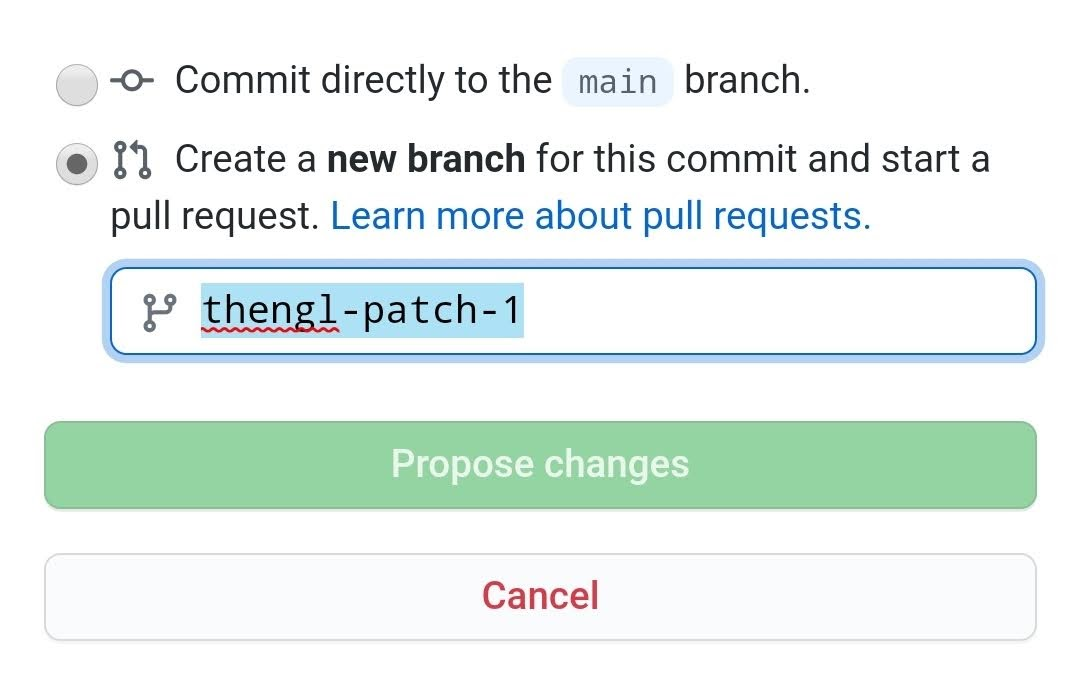
\includegraphics[width=0.5\linewidth]{img/example_pull_request} 

}

\caption{Example of a pull request on Github.com.}\label{fig:pull-request}
\end{figure}

If you're new to markdown and want to learn how to use it, please refer to \href{https://guides.github.com/features/mastering-markdown/}{this tutorial}.

If you are new to R and/or \href{https://cran.r-project.org/web/views/Environmetrics.html}{\textbf{environmetrics}}, please consider reading / studying:

\begin{itemize}
\tightlist
\item
  Kabacoff, R.I., (2011). \href{https://www.statmethods.net/}{R in Action: Data Analysis and Graphics with R}. Manning publications, ISBN: 9781935182399, 472 pages.\\
\item
  Grolemund, G., (2014). Hands-On Programming with R. O'Reilly, \url{https://github.com/rstudio-education/hopr}\\
\item
  \href{http://www.rstudio.com/products/RStudio/}{RStudio},
\end{itemize}

If you'd like more of a roadmap to guide you through R, have a look at Oscar's blogpost:

\begin{itemize}
\tightlist
\item
  \url{https://oscarbaruffa.com/a-roadmap-for-getting-started-with-r/}
\end{itemize}

\hypertarget{video-course-getting-started-with-r}{%
\section{Video Course: Getting started with R}\label{video-course-getting-started-with-r}}

If you prefer video instruction with progress tracking:

\begin{itemize}
\tightlist
\item
  \url{https://rfortherestofus.com/courses/getting-started/}
\end{itemize}

\hypertarget{compendium-of-global-gridded-environmental-data-sets}{%
\chapter{Compendium of Global Gridded Environmental Data Sets}\label{compendium-of-global-gridded-environmental-data-sets}}

This is an open compendium of global (gridded) environmental datasets (bio-geophysical variables). Here you can
find systematic listings of published data sets (a selection of the cutting-edge datasets we plan to upload to OpenLandMap.org)
with emphasis on publicly available data sets available under open data license. These reviews are periodically
maintained by the \href{https://openlandmap.org/}{www.OpenLandMap.org} development team and
collaborators. They are only meant to serve as general inventories of what is
available, and NOT as an in-depth review article.

To contribute to this portal, consider submitting new data by editing this Markdown document.
Please check also the working version of the \href{https://docs.google.com/spreadsheets/d/1SX51OilNt-cUYpAa7t0LAvZRTzq3Sd4WJLnX6mWKfQk/edit?usp=sharing}{OEMC global Land Use Land Cover Taxonomy Tables}.

If your work / products are cited here, you are for us \textbf{a champion of open environmental data} and
we are enormously thankful for your contributions (please never stop!).

Minimum conditions to include your contribution to this compendium:

\begin{itemize}
\tightlist
\item
  Please submit / register \textbf{only global data sets} (at least 80\% complete; at least 5 continents);
\item
  The data sets should be peer-reviewed or at least come with fully documented processing steps / metadata and/or an official technical report;
\item
  Refer to computational notebooks or materials that explain how was the data produced: follow as much as possible the \textbf{\href{https://en.wikipedia.org/wiki/Open_science}{open science}} principles;
\item
  The data set should have one of the compatible \textbf{\href{https://opendefinition.org/licenses/}{open data licenses}} or at least allow for the derivative works to be released as open data;
\item
  The data set should be current i.e.~still in use and the citation / URL should mention the most recent update;
\item
  Mention of the data should focus on practical things such as \emph{``where I can read about how was this data set produced?''}, \emph{``where can I download this data?''}, \emph{``what are its technical characteristics such as spatial resolution, temporal coverage, biophysical variables and measurement units?''};
\end{itemize}

Here are the top 5 technical aspects of the data that should be clear to reader without confusion:

\begin{enumerate}
\def\labelenumi{\arabic{enumi}.}
\tightlist
\item
  What is the DOI of the data set i.e.~what is the permanent URL from which it can be accessed and downloaded?
\item
  What is the spatial resolution / effective scale of the data set? We recommend to avoid using abstract metrics such as ``3-arcseconds'' or similar but use instead round metrics e.g.~``90-m spatial resolution''.
\item
  Which referent time-period does the data set covers / what is the time-span of the training or input data?
\item
  What is the \#1 technical documentation for this data set (ideally a peer-review publication DOI or similar)?
\item
  For which purpose can/should this data set be used and what is its significance?
\end{enumerate}

Examples of contributions that will not be welcomed:

\begin{itemize}
\tightlist
\item
  Registering and submitting regional or local data sets i.e.~covering only continents or countries;
\item
  Mentioning, listing and/or self-promoting of proprietary / commercial data sets will not be accepted;
\item
  Rating or criticizing data sets or expressing personal opinions;
\item
  Deleting text submitted by others or inserting code that is computational or difficult to maintain;
\end{itemize}

You can however mention some data sets that are not open if they are without any open data / open source alternative.

\hypertarget{thematic-data-groups}{%
\section{Thematic data groups:}\label{thematic-data-groups}}

All layers are organized around the following themes
(based on the \href{https://ggim.un.org/meetings/GGIM-committee/9th-Session/documents/Fundamental_Data_Publication.pdf}{UN-GGIM The Global Fundamental Geospatial Data Themes}):

\begin{itemize}
\tightlist
\item
  \textbf{Buildings and Settlements}: includes administrative and socio-economic data, natural hazards and similar,
\item
  \textbf{Elevation and Depth}: includes Digital Terrain Models and DEM-derived parameters, LiDAR point clouds, canopy heights, hydrological data derived from DTMs and similar,
\item
  \textbf{Geology and Soils}: includes geological, surface lithology and soil property and class maps,
\item
  \textbf{Land Cover and Land Use}: includes land cover / land use classes, land cover change and drivers of land use / land cover change,
\item
  \textbf{Population Distribution}: includes population density and population variables, urbanization and lights at night images,
\item
  \textbf{Water}: includes surface and underground water resources and similar,
\item
  \textbf{Physical Infrastructure}: includes road and rail networks, dams, industrial facilities and similar,
\item
  \textbf{Climate}: includes long-term climatic images, climatic time-series data, future climate predictions and meteorological images,
\item
  \textbf{Biodiversity and Nature Conservation}: includes wildlife resources, protected areas, natural vegetation and biomes, ecoregions and biodiversity maps,
\end{itemize}

This list is not universal and might need to be updated and improved. For comparison, \href{https://www.earthdata.nasa.gov/eosdis}{NASA's EarthData}
portal distinguishes the following global data themes:

\begin{itemize}
\tightlist
\item
  Atmosphere;
\item
  Biosphere;
\item
  Cryosphere;
\item
  Human Dimensions;
\item
  Land Surface;
\item
  Ocean;
\item
  Solid Earth;
\item
  Sun-Earth Interactions;
\item
  Terrestrial Hydrosphere;
\end{itemize}

\hypertarget{other-repositories-of-global-open-environmental-layers}{%
\section{Other repositories of global (open) environmental layers}\label{other-repositories-of-global-open-environmental-layers}}

Sorted alphabetically:

\begin{itemize}
\tightlist
\item
  \href{https://registry.opendata.aws/tag/earth-observation/}{Amazon AWS Open EO Data};
\item
  \href{https://land.copernicus.eu/global/}{Copernicus Global Land Service} --- global data sets (bio-geophysical products) produced by the Land Monitoring Core Service (LMCS) of Copernicus, the European flagship programme on Earth Observation;
\item
  \href{https://geoservice.dlr.de/web/maps}{DLR Geoportal};
\item
  \href{http://earthenv.org/}{EarthEnv.org} --- Global, remote-sensing supported environmental layers for assessing status and trends in biodiversity, ecosystems, and climate (hosted by Yale University / NASA and others);
\item
  \href{https://livingatlas.arcgis.com/en/home/}{ESRI ArcGIS Living Atlas of the World};
\item
  \href{https://collections.eurodatacube.com/}{Euro Data Cube Public Collections} --- a series of global data sets primarily based on the Copernicus programme / Sentinel satellites;
\item
  \href{http://www.fao.org/geonetwork/srv/en/main.home}{FAO's GeoNetwork} --- serves a diversity of data produced by FAO run or supported projects at a diversity of scales;
\item
  \href{http://freegisdata.rtwilson.com/}{Free GIS data compendium} by R.T. Wilson;
\item
  \href{http://www.geoportal.org/}{GeoPortal.org} --- The Global Earth Observation System of Systems (GEOSS) portal implemented and operated by the European Space Agency (typically only a catalog of data sets / no or limited data is hosted);
\item
  \href{https://glad.geog.umd.edu/}{Global Land and Discovery group} --- University of Maryland Global Land and Discovery group (GLAD) group global data sets,
\item
  \href{https://developers.google.com/earth-engine/datasets}{Google Earth Engine Data Catalog} --- Google's repository of global and local data sets;
\item
  \href{https://modis.gsfc.nasa.gov/data/dataprod/}{MODIS Land products} usually at moderate resolutions from 250-m to 1-km (also available for searching via \url{https://lpdaac.usgs.gov/product_search/});
\item
  \href{https://earthobservatory.nasa.gov/global-maps}{NASA Earth Observation (NEO)} is part of the \href{http://eospso.nasa.gov/}{EOS Project Science Office} located at NASA Goddard Space Flight Center;
\item
  \href{https://www.earthdata.nasa.gov/eosdis}{NASA's Earth Observing System Data and Information System (EOSDIS)} provides tools to find and access global data sets produced by NASA and aiming at Earth System Science;
\item
  \href{http://www.naturalearthdata.com/downloads/}{Natural Earth Data} website compiled by Nathaniel Vaughn (KELSO) and volunteers;
\item
  \href{https://github.com/opengeos/geospatial-data-catalogs}{Open Geospatial Catalogs} a list of open geospatial datasets available on AWS, Earth Engine, Planetary Computer, NASA CMR, and STAC Index;
\item
  \href{https://opendata.oraclecloud.com/}{Oracle Open Data Repository (geospatial)};
\item
  \href{https://daac.ornl.gov/get_data/}{ORNL DAAC} The Oak Ridge National Laboratory Distributed Active Archive Center (ORNL DAAC) for Biogeochemical Dynamics is a NASA Earth Observing System Data and Information System (\href{https://earthdata.nasa.gov/eosdis/daacs}{EOSDIS}) data center managed by the Earth Science Data and Information System (\href{https://earthdata.nasa.gov/esds}{ESDIS}) Project;
\item
  \href{https://overturemaps.org/download/}{Overture Maps} by the Overture Maps Foundation serves some basic admin layers e.g.~buildings, road networks, places etc all as open data.
\item
  \href{http://www.sage.wisc.edu/atlas/maps.php}{SAGE Atlas of the Biosphere portal};
\item
  \href{https://sedac.ciesin.columbia.edu/data/sets/browse}{SEDAC} --- A Data Center in NASA's Earth Observing System Data and Information System (EOSDIS) --- Hosted by CIESIN at Columbia University;
\item
  \href{https://stacindex.org/catalogs}{STAC index} an international telephone book for STAC Catalogs, Collections, APIs, Software and Tools (you can also add your own data and tools to the list);
\item
  \href{https://gee-community-catalog.org/}{The awesome-gee-community-catalog} by Samapriya Roy et al.;
\item
  \href{http://geodata.grid.unep.ch/}{UNEP/GRID GEO DataPortal} and \href{http://maps.grida.no/region/global}{UNEP/GRID-Arendal} --- a large repository of global grids at various resolutions;
\item
  \href{https://datacatalog.unep.org/app/}{UNEP Data Catalog};
\item
  \href{https://resourcewatch.org/data/explore}{World Resources Institute (WRI) Resource Watch} --- features hundreds of data sets all in one place on the state of the planet's resources and citizens.
\item
  \href{http://earthtrends.wri.org/}{World Resources Institute (WRI) Environmental Information Portal} serves a number of global grids derived by the WRI and collaborators;
\end{itemize}

\begin{figure}

{\centering 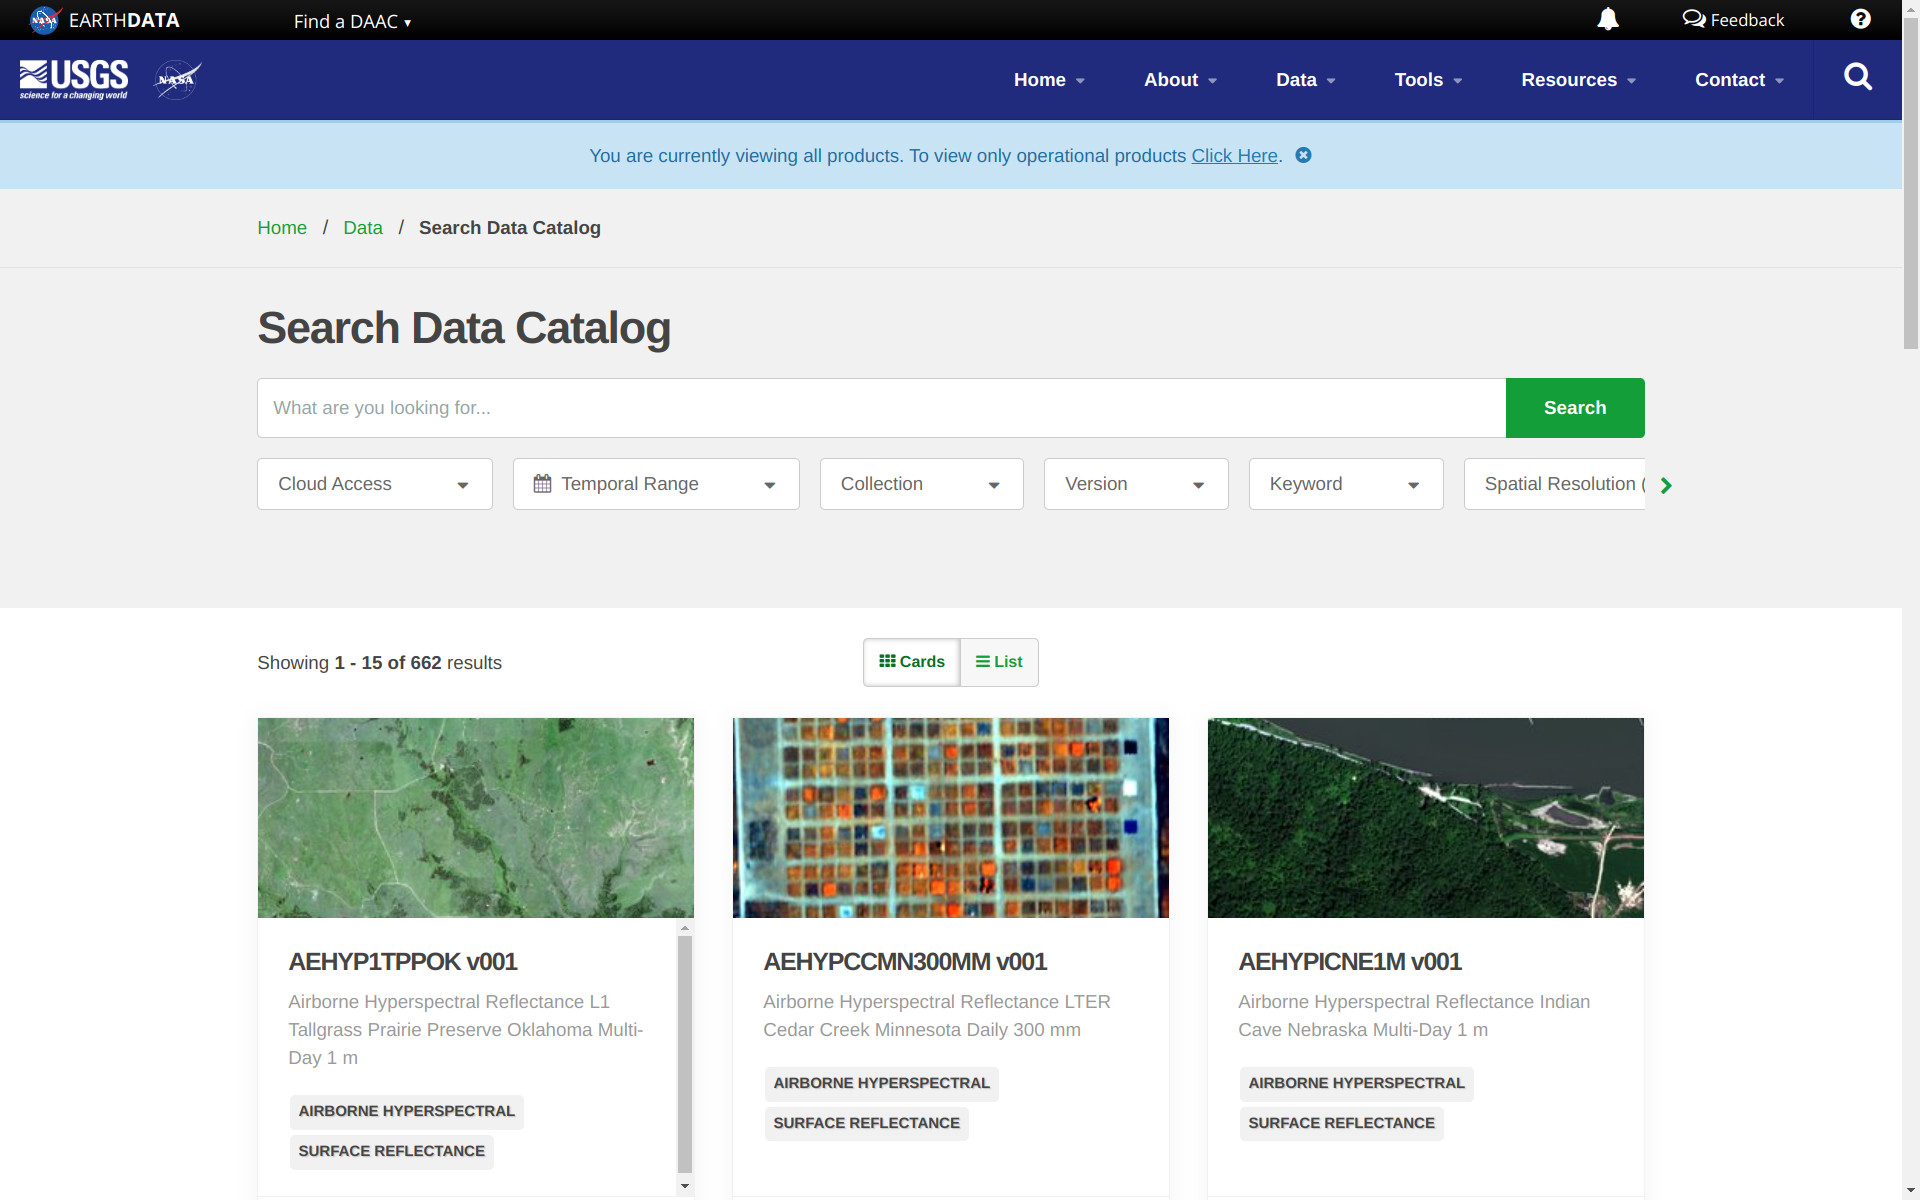
\includegraphics[width=1\linewidth]{img/lpdaac_usgs_preview} 

}

\caption{LP DAAC data catalog is an example of continuosly updated and complete catalog of global environmental data (primarily based on MODIS and similar EO missions) which are available publicly without restrictions.}\label{fig:usgs-modis}
\end{figure}

\hypertarget{make-your-data-more-accessible-more-usable}{%
\section{Make your data more accessible more usable}\label{make-your-data-more-accessible-more-usable}}

If you are making open global data aiming at enabling others
to do more advanced analysis \& eventually help with better management of
natural resources, what are the key steps to improve usability of
your data? Within the \href{https://earthmonitor.org/}{Open-Earth-Monitor project} we specifically
looked at hundreds of cases of data sets that have a high potential
but are somewhat under-used or not used at all because of poor documentation,
being incomplete or requiring specialized knowledge. This is what we believe is especially
important to help boost usability and accessibility of your global geospatial data:

\begin{itemize}
\tightlist
\item
  Aim at making your data \textbf{\href{https://medium.com/mlearning-ai/present-and-future-of-data-cubes-an-european-eo-perspective-735d3f16f7c9}{4C-ARCO}}: complete, consistent, current and correct, then on top of it \textbf{Analysis-ready and Cloud Optimized (ARCO)};
\item
  Use \textbf{(open) cloud-native data formats} to distribute data (especially for large data) either \href{https://www.cogeo.org/}{COG's}, \href{https://radiant.earth/blog/2023/06/exploring-the-potential-of-geozarr-for-storage-and-analysis/}{GeoZarr}, \href{https://docs.xarray.dev/en/stable/}{XArray} and/or \href{https://geoparquet.org/}{Geoparquet} / \href{https://flatgeobuf.org/}{Flatgeobuf} and similar for tabular / vector data;
\item
  Optimize compression of the data so that data download is as fast as possible; for example, compression is by default already included in the \href{https://www.cogeo.org/}{Cloud-Optimized GeoTIFF data format};
\item
  Use \textbf{\href{https://stacspec.org/en}{SpatioTemporal Asset Catalogs (STAC)}} or similar to register data and the access points (usually also requires that you publish your data via a Simple Storage Service (S3));
\item
  Best technical documentation for the data is (A) a peer-review publication, and (B) a \href{https://www.datacamp.com/blog/jupyter-and-r-markdown-notebooks-with-r}{computational notebook} providing a demo of the method used and key results; a peer-review publication increases confidence for non-experts; computational notebooks help increase quality as people then try to extend your work, then discover and report problems and help you make revisions;
\item
  Always register all versions of your data so that anyone can track fixes and improvements; for each version try to obtain DOI, so that it is also kept for ever;
\item
  Try to register your data in some higher level aggregator such as \href{https://stacindex.org/}{STAC index} (or this compendium!);
\item
  Test if your data can be easily used in most-popular GIS software such as \href{https://www.cogeo.org/qgis-tutorial.html}{QGIS}: does it have the right legend? can users quickly find metadata, explanation of units, how was the map produced?
\item
  Provide support and regularly update your data; like with software no data is bug-free, by updating and improving your data your user community learns to appreciate your efforts and builds higher trust;
\end{itemize}

Of course, not every version or testing of your data / mapping skills
needs to be registered with unique DOI. Also, writing metadata \&
computational notebooks requires time and resource investments, so you
need to plan carefully your time.

Here are also some world-leading providers of tools for making geospatial
data more usable and more \textbf{\href{https://www.go-fair.org/fair-principles/}{FAIR} (Findable, Accessible, Interoperable, and Reusable)} (unsorted):

\begin{itemize}
\tightlist
\item
  \url{https://gdal.org} software backbone of any open geospatial data project;
\item
  \url{https://radiant.earth/} is organization largely behind COGs and STAC;
\item
  \url{https://pangeo.io/} a project developing tools for Big Data geoscience;
\item
  \url{https://github.com/opengeospatial} the Open Geospatial Consortium repositories hosting many open source solutions for Big Data geoscience;
\item
  \url{https://github.com/opengeos/} a collection of open-source software packages for the geospatial community;
\item
  \url{https://r-spatial.org/} and \url{https://rspatial.org/} packages and tutorials for accessing and processing geospatial data using R;
\item
  \url{https://juliageo.org/} libraries for Julia language to support processing geospatial data;
\end{itemize}

\hypertarget{buildings-and-settlements}{%
\section{Buildings and Settlements}\label{buildings-and-settlements}}

\hypertarget{administrative-and-socio-economic-data}{%
\subsection{Administrative and socio economic data}\label{administrative-and-socio-economic-data}}

Administrative data can be used to calculate proximity-based parameters and to
orient the users geographically. One publicly accessible global administrative
data database is the \href{http://gadm.org/}{GADM} database of \textbf{Global Administrative Areas}.
It comprises borders of countries and lower level subdivisions such as provinces
and counties (more than 100,000 areas). Lower level administrative boundaries can
be obtained via the \href{http://www.fao.org/geonetwork/srv/en/main.home}{FAO's GeoNetwork server}.
Even more detailed is the \textbf{\href{https://data.apps.fao.org/map/catalog/static/search?keyword=HiH_boundaries}{FAO GAUL: Global Administrative Unit Layers}} which is
available for different periods and up to the 3rd admin level, so one can potentially
also track changes in political units (the \href{https://github.com/openlandmap/book/blob/master/tabular/GAUL_g2015_2014_1_legend.csv}{table} \texttt{GAUL\_g2015\_2014\_1\_legend.csv}
contains an example of cca 3500 administrative units with codes). The \href{http://www.geoboundaries.org/}{geoBoundaries}
is a global Database of Political Administrative Boundaries and contains a snapshot
of political and administrative boundaries since 2017.

An important global vector dataset is the \textbf{\href{https://shoreline.noaa.gov/data/datasheets/wvs.html}{World Vector Shoreline}}
data set at scale 1:250,000 \citep{carlotto2017enhancing}. This can be, for example,
used to derive the global distance from the sea coast line map and similar.

The \textbf{\href{https://overturemaps.org/download/}{Overture Maps foundation}} provides up-to-date (current) global vectors on
Layers of interest include: admins, base, buildings, places etc. You can simply \href{https://github.com/OvertureMaps/data/}{download}
the data for are of interest, then convert to \href{https://msbarry.github.io/planetiler-overture-demo/}{PMTiles} or similar, then add to your back-end/front-end as a clickable layer.

The \textbf{\href{https://geoservice.dlr.de/web/maps/eoc:wsf}{World Settlement Footprint (WSF)}} is a series of datasets that provide comprehensive, high-resolution mapping of human settlements across the globe. WSF is a 10-m resolution binary mask outlining the extent of human settlements globally derived from 2014--2015 multitemporal Landsat-8 and Sentinel-1 imagery (\href{https://geoservice.dlr.de/web/maps/eoc:wsf}{WFS2015}) and 2019 multitemporal Sentinel-1 and Sentinel-2 imagery (\href{https://geoservice.dlr.de/web/maps/eoc:wsf2019}{WFS 2019}). \href{https://geoservice.dlr.de/web/maps/eoc:wsfevolution}{WSF Evolution} is a 30-m resolution dataset outlining the global settlement extent on a yearly basis from 1985 to 2015.

The \href{https://sedac.ciesin.columbia.edu/data/sets/browse}{Socioeconomic Data and Applications Center (SEDAC)} a Data Center in NASA's Earth
Observing System Data and Information System (EOSDIS) Hosted by CIESIN at Columbia University
has produced a number of open global socio-economic data sets including on themes such as: Agriculture, Climate, Conservation,
Governance, Hazards, Health, Infrastructure, Land Use, Marine and Coastal, Population,
Poverty, Sustainability, Urban and Water.

\hypertarget{elevation-and-depth}{%
\section{Elevation and Depth}\label{elevation-and-depth}}

\hypertarget{digital-terrain-models}{%
\subsection{Digital Terrain Models}\label{digital-terrain-models}}

Global Shuttle Radar Topography Mission (SRTM) \href{http://en.wikipedia.org/wiki/Digital_elevation_model}{Digital Elevation Model} is
on of the most well-known global environmental dataset \citep{rabus2003shuttle}
available with a resolution of approximately 30-m (1 arcsec). The most recent
version of the SRTM DEM is the \href{https://lpdaac.usgs.gov/products/nasadem_hgtv001/}{NASADEM}.
In 2018 two new global elevation models were produced:

\begin{itemize}
\tightlist
\item
  ESA's \textbf{\href{https://doi.org/10.5270/ESA-c5d3d65}{Copernicus DEM GLO-30}} at 30-m resolution;
\item
  JAXA's \textbf{\href{https://www.eorc.jaxa.jp/ALOS/en/dataset/aw3d30/aw3d30_e.htm}{ALOS AW3D30}} at 30-m resolution;
\end{itemize}

Both ALOS AW3D and GLO-30 are the new generation surface models. Both need removal
of canopy and buildings before they can be used as terrain models i.e.~for surface water runoff and similar.
\citet{MERITDEM} has produced \textbf{MERIT DEM} and \textbf{MERIT Hydro}, actual DTM post-filtered and hydrologically
correct DTM. Both are available for \href{https://hydro.iis.u-tokyo.ac.jp/~yamadai/MERIT_Hydro/}{download} under open data license but only at 90/100-m resolution. Using the MERIT DEM, \citet{amatulli2020geomorpho90m} have produced \textbf{\href{https://doi.org/10.5069/G91R6NPX}{Geomorpho90m}} and
\href{https://doi.org/10.18728/igb-fred-762.1}{Hydrography90m} \citep{amatulli2022hydrography90m} data sets.

A complete land surface model ETOPO1 Global Relief Model (includes bathymetry data)
is available at resolution of 1-km and can be obtained from the \href{http://ngdc.noaa.gov/}{NOAA's National Geophysical Data Center} \citep{amante2009etopo1}.
An updated version of the ETOPO is the Global Land One-km Base Elevation Project (\href{http://www.ngdc.noaa.gov/mgg/topo/globe.html}{GLOBE}) DEM. Global bathymetry data (\textbf{\href{http://www.gebco.net/data_and_products/gridded_bathymetry_data/}{GEBCO data set}}) can also obtained from the British Oceanographic Data Centre.

\href{https://portal.opentopography.org/dataCatalog?group=global}{OpenTopography.org} maintains a catalog of
global elevation data sets including national data sets. A combination (Ensemble-DTM) of
GLO-30, AW3D30, MERIT DEM and number of continental / national DTM's is available via \href{https://stac.openlandmap.org/dtm.bareearth_ensemble/collection.json}{OpenLandMap.org}.

\citet{iwahashi2007automated} produced a global landform type map of the world at 250-m.
\textbf{Geomorphological forms} (Geomorphon classification system) at 100-m are also available for download
via the \href{https://doi.org/10.5069/G91R6NPX}{OpenTopography.org} repository and/or \href{https://zenodo.org/doi/10.5281/zenodo.1447198}{Zenodo}.
\citet{Frye2023} produced \textbf{\href{https://www.esri.com/arcgis-blog/products/arcgis-living-atlas/announcements/introducing_nlwv2/}{Named Landforms of the World (NLW2)}} with most of data at 250-m resolution.

\hypertarget{canopy-height-data}{%
\subsection{Canopy height data}\label{canopy-height-data}}

There are several global reference point data set and products that represent canopy height (often
including heights of building / human-built structures). Currently the two global
public reference data sets / missions for monitoring canopy height and morphological ecosystem
parameters are:

\begin{itemize}
\tightlist
\item
  \href{https://gedi.umd.edu/}{Global Ecosystem Dynamics Investigation (GEDI) data set};
\item
  \href{https://openaltimetry.earthdatacloud.nasa.gov/data/}{ICESat, ICESat-2 data sets};
\end{itemize}

You can visually explore and download the ICESat data from \url{https://www.openaltimetry.org}.
GEDI and ICESat can be used to derive number of ecosystem parameters including biomass
density (above ground), canopy height, terrain height, LAI, canopy structure etc.
The complete global gridded canopy height / biomass density products include:

\begin{itemize}
\tightlist
\item
  \textbf{\href{https://glad.umd.edu/dataset/gedi/}{Global forest canopy height maps at 30-m}} produced by GLAD \citep{POTAPOV2021112165};
\item
  \textbf{\href{https://langnico.github.io/globalcanopyheight/}{Global 10-m resolution canopy height map}} \citep{lang2023high};
\item
  \textbf{\href{https://doi.org/10.6084/m9.figshare.c.4561940}{Global 100-m resolution aboveground biomass carbon density}} \citep{Spawn2020};
\item
  \textbf{\href{https://daac.ornl.gov/cgi-bin/dataset_lister.pl?p=40}{GEDI L4B}} gridded aboveground biomass density (nominal latitude extent of -52 to 52 degrees) at 1-km resolution \citep{Dubayah2023};
\end{itemize}

\textbf{\href{https://geoservice.dlr.de/web/maps/tdm:dcm30}{TanDEM-X 30-m DEM Change Maps (DCM)}} shows significant changes in elevation (usually canopy height) for the period 2016 to 2022.
DLR warns that users must be aware that a given elevation change measured in the DEM change maps corresponds to a topographic change with respect to TanDEM-X 30m EDEM, i.e.~this is only an estimate of physical height change.

\hypertarget{hydrological-hydrographic-data}{%
\subsection{Hydrological / hydrographic data}\label{hydrological-hydrographic-data}}

World river and stream networks (vector files) are available from the \textbf{\href{https://www.hydrosheds.org/page/gloric}{Global River Classification (GLORIC) DB}}.
A \href{https://zenodo.org/doi/10.5281/zenodo.3355006}{rasterized version of this data set} is available at resolution of 250-m.
\textbf{\href{http://hydro.iis.u-tokyo.ac.jp/~yamadai/MERIT_Hydro}{MERIT Hydro}} also provides Upstream Drainage Area at 100-m global and should be considered a reference at this scale \citep{MERITDEM}.
\citet{amatulli2022hydrography90m} describes Hydrography90m (global hydrographic dataset) although this is
not available as open data (authors used the NC-license).

\textbf{Global reservoirs (GRanD)} (polygons) dataset can be obtained from the \href{https://www.globaldamwatch.org/directory}{Global Dam Watch website}.
Connected to GRanD, \textbf{Global reservoir bathymetry estimate (ReGeom)} dataset is available from \href{https://zenodo.org/doi/10.5281/zenodo.1322883}{zenodo}.
\textbf{Global streamflow time series dataset} i.e.~the GRDC's (Global Runoff Data Centre) streamflow observations (cca 11,000 stations) can be downloaded from the \href{https://portal.grdc.bafg.de/}{GRDC data portal}.

\citet{lehner2013global} provide a global river hydrography and river network routing data set (HydroBASINS and \textbf{\href{https://www.hydrosheds.org/hydrosheds-core-downloads}{HydroSHEDS}}) at 500-m spatial resolution.
\citet{lane2023mapping} produced a global 90-m resolution map of \textbf{\href{https://doi.org/10.23719/1528331}{Non-Floodplain Wetland (Global NFW)}}.
Global NFW is based on multiple input data sources including MERIT Hydro,
HydroBASINS and similar.

Several data set exists that quantify global surface water extent and type, wetlands distribution and
fresh-water resources in general:

\begin{itemize}
\tightlist
\item
  \textbf{\href{https://global-surface-water.appspot.com/}{JRC's global surface water dynamics data set at 30-m}}: this includes occurrence probability of surface water, surface water extent and change 1984--2021 \citep{Pekel2016};
\item
  \textbf{\href{https://glad.umd.edu/dataset/global-surface-water-dynamics}{GLAD's global surface water dynamics 1999--2021}} at 30-m resolution providing also map of 7 types of surface water stable and change dynamics \citep{pickens2020mapping};
\item
  \textbf{\href{https://doi.org/10.1594/PANGAEA.892657}{Multi-source global wetland map at 500-m resolution}} \citep{tootchi2019multi}
\end{itemize}

DLR's (MODIS-based) \textbf{\href{https://geoservice.dlr.de/web/maps/eoc:gwp:yearly}{Global WaterPack (GWP) monthly and yearly}} product (different water coverage categories) at 250-m spatial resolution
is available for the period 2003 to 2022+.

\href{https://www.earthdata.nasa.gov/eosdis/daacs/podaac}{NASA's Physical Oceanography Distributed Active Archive Center} (PO.DAAC) serves
data on ocean winds, sea surface temperature, ocean surface topography, sea surface salinity, surface water and similar.

\hypertarget{geology-and-soils}{%
\section{Geology and Soils}\label{geology-and-soils}}

\hypertarget{geology-and-lithology}{%
\subsection{Geology and lithology}\label{geology-and-lithology}}

The current global geological map approved by the Commission for the Geological Map of
the World is the \href{https://ccgm.org/en/}{1:25M Geological Map of the World} (maps not available publicly).
The world geological maps are now being integrated via the \href{http://www.onegeology.org/}{OneGeology}
project which aims at producing a consistent Geological map of the world in approximate scale 1:1M \citep{jackson2010onegeology};
progress can be followed via the interactive \href{http://portal.onegeology.org/}{OneGeology portal}.

USGS has several \href{http://energy.usgs.gov/}{data portals}, e.g.~that allow browsing
of the \href{https://certmapper.cr.usgs.gov/data/apps/world-maps/}{International Surface Geology}
(split into South Asia, South America, Iran, Gulf of Mexico, Former Soviet Union, Europe, Carribean, Bangladesh, Asia Pacific, Artic, Arabian Peninsula, Africa and Afganistan).
\citet{hartmann2012new} have assembled a global, purely lithological database called \textbf{GLiM} (\href{https://www.geo.uni-hamburg.de/geologie/forschung/aquatische-geochemie/glim.html}{Global Lithological Map}).
GLiM consists of over 1.25 million digital polygons with classified in three levels (a total of 42 rock-type classes).

USGS, jointly with ESRI, have released in 2014 a \textbf{\href{https://www.esri.com/about/newsroom/insider/the-first-detailed-ecological-land-unitsmap-in-the-world/}{Global Ecological Land Units map}}
at 250-m resolution. This also includes a world layer of rock types. The data can
be downloaded from the \href{http://rmgsc.cr.usgs.gov/outgoing/ecosystems/Global/}{USGS site} or via \href{https://zenodo.org/doi/10.5281/zenodo.1447198}{Zenodo}.

\citet{fan2013global} produced global maps of \textbf{Groundwater Table Depth} that has been systematically updated in 2022.
The modeled monthly water table depth can be \href{http://thredds-gfnl.usc.es/thredds/catalog/GLOBALWTDFTP/catalog.html}{downloaded for each continent}.
\citet{cuthbert2019global} produced water table ratio and groundwater response times maps at 1-km resolution (available from \href{https://doi.org/10.6084/m9.figshare.7393304}{figshare}).
The International Groundwater Resources Assessment Centre (IGRAC) maintains the
\href{https://ggis.un-igrac.org/}{Global Groundwater Information System (GGIS)}. IGRAC is
aiming at producing \href{https://sdgs.un.org/partnerships/produce-and-disseminate-open-global-groundwater-datasets}{global groundwater datasets}.

\citet{tang2023global} made a global inventory (polygon map) of mining areas (\textbf{global mine area coverage}):
The polygons cover about about 66,000 km-square of features like
waste rock dumps, pits, water ponds, tailings dams, heap leach
pads and processing/milling infrastructure.
The data is available from \href{https://doi.org/10.5281/zenodo.6806817}{zenodo}.
An update of the global mining areas (three layers: mining polygons, mining centroids,
mining area per grid cell) is provided by \citet{maus2022update}; the data set is available via
\href{https://doi.org/10.1594/PANGAEA.942325}{PANGAEA}; also available via \url{https://fineprint.global/viewer}.

\hypertarget{earthquakes-natural-hazards}{%
\subsection{Earthquakes / natural hazards}\label{earthquakes-natural-hazards}}

Natural hazards include:

\begin{itemize}
\tightlist
\item
  Earthquakes,
\item
  Volcanoes,
\item
  Landslides,
\item
  Famines \& Droughts,
\item
  Hurricanes, Tornados, and Cyclones,
\item
  Extreme precipitation and flooding,
\item
  Extreme Temperature (Heat \& Cold),
\item
  Wildfires,
\end{itemize}

A number of institutions have jointly produced a \href{https://www.gfz-potsdam.de/gshap}{Global Seismic Hazard map} \citep{shedlock2000gshap}.
This map, although slightly outdated and of limited detail, can be obtained directly
from the GSHAP project \href{https://www.gfz-potsdam.de/gshap}{webite}. From the
\href{http://ngdc.noaa.gov/hazard/earthqk.shtml}{NOAA's National Geophysical Data Center} one
can obtain a point map with all major earth quakes (\textbf{Significant Earthquake Database}; cca 5000 quakes),
and generate a (kernel density) map for Earthquake magnitude.

University of Hawaii maintains a \href{https://www.pdc.org/risk-and-vulnerability/}{Global Hazards Information Network},
which contains a number of global layers including a \href{https://hub.arcgis.com/datasets/esri-de-content::world-airports}{map of Global Airports}, locations of \href{https://earthquake.usgs.gov/earthquakes/browse/significant.php}{significant earthquakes} and earthquake zones.

Copernicus Global Land Service distributes a global assessment of \textbf{\href{https://land.copernicus.eu/global/products/ba}{Burnt Area}}
at 300-m spatial resolution, but available only from 2019 onwards.
NASA's \href{https://firms.modaps.eosdis.nasa.gov/map/}{FIRMS (Fire Information for Resource Management System)} provides
real-time access to occurrence of fires including access to the \href{https://firms.modaps.eosdis.nasa.gov/download/}{archive data}.
\href{https://www.earthdata.nasa.gov/eosdis/daacs/ghrc}{NASA's Global Hydrometeorology Resource Center Distributed Active Archive Center (GHRC DAAC)} serves global data on
lightning, tropical cyclones, and storm-induced hazards through integrated collections of satellite, airborne, and in-situ data sets.

NOAA's \href{https://www.drought.gov/international}{Global Drought Information System (GDIS)} serves global estimates of drought conditions.
Maps are usually only available at coarse resolution of 25, 10 or 5-km or similar.

\hypertarget{soils}{%
\subsection{Soils}\label{soils}}

Soil maps (physical, chemical, biological soil properties and soil classes) are especially important for spatial prediction of distribution
of vegetation and (plant) species distribution.
FAO, IIASA, ISRIC, ISSCAS, JRC have produced in 2007 a 1-km resolution gridded
soil-class map, produced by merging various national soil maps. This product is
also known as the \textbf{\href{https://www.fao.org/soils-portal/data-hub/soil-maps-and-databases/harmonized-world-soil-database-v20/en/}{Harmonized World Soil Database}}.
Global predicted WRB soil type maps at 1-km can be download as geotifs from \href{https://doi.org/10.5281/zenodo.7820796}{here}.
USGS / USDA have produced a map of \href{https://www.nrcs.usda.gov/conservation-basics/natural-resource-concerns/soils/soil-geography}{Global Soil Regions}
map at resolution of 60 arcsec, and which is based on the FAO-UNESCO soil map.

A list of seven gridded soil property maps (at resolution of 5 arc-minutes i.e.~about 10-km) ---
soil-carbon density, total nitrogen density, field capacity, wilting point, profile
available water capacity, thermal capacity, and bulk density --- is available via the \href{https://daac.ornl.gov/SOILS/guides/IGBP-DIS.html}{International Geosphere-Biosphere Program Data and Information System (IGBP-DIS) data set}. Some additional soil property maps such as \href{https://sage.nelson.wisc.edu/data-and-models/atlas-of-the-biosphere/mapping-the-biosphere/ecosystems/}{pH} and \href{https://sage.nelson.wisc.edu/data-and-models/atlas-of-the-biosphere/mapping-the-biosphere/ecosystems/}{soil moisture}, can
be also obtained from the \href{https://sage.nelson.wisc.edu/data-and-models/atlas-of-the-biosphere/}{Atlas of Biosphere project}.
\textbf{\href{http://globalchange.bnu.edu.cn/research/soilw}{Global Soil Dataset for Earth System Model (GSDE)}} contains the largest
number of soil properties (gridded) at 1-km spatial resolution \citep{Shangguan2014}.

FAO's Global Soil Partnership has produced a \textbf{\href{https://doi.org/10.4060/ca7597en}{Global Soil Organic Carbon Map (GSOCmap)}} at 1-km resolution.
ISRIC --- World Soil Information maintains \href{http://www.isric.org/wosis}{a global soil profile database (WoSIS)}
with over 100,000 profiles and over 50 analytical and descriptive parameters \citep{batjes2020standardised}. Predictions of soil properties (GeoTIFFs) at spatial resolution of
250-m or better are available from multiple sources including:

\begin{itemize}
\tightlist
\item
  \textbf{\href{https://www.isric.org/explore/soilgrids}{SoilGrids}} \citep{poggio2021soilgrids};
\item
  \textbf{\href{https://developers.google.com/earth-engine/datasets/tags/openlandmap}{OpenLandMap.org soil properties and classes}};
\item
  \textbf{\href{https://www.futurewater.eu/projects/hihydrosoil/}{HiHydroSoil: Global Maps of Soil Hydraulic Properties}} (available upon request or directly \href{https://code.earthengine.google.com/?scriptPath=users/sat-io/awesome-gee-catalog-examples:soil-properties/HiHYDRO-SOIL-LAYERS}{via GEE});
\end{itemize}

\href{https://crowtherlab.com/maps/\#/}{Crowther's lab} distributes a number of soil-biology global data sets (1-km)
including maps of soil nematodes density, bacterial biomass, fungal biomass and similar.

Some soil properties are often directly estimated from the EO data. For example the soil moisture
\textbf{\href{http://glass.umd.edu/soil_moisture/}{GLASS SM data set}} and the \href{https://doi.org/10.11888/RemoteSen.tpdc.272760}{gap-free global daily surface soil moisture at 1-km grid resolution}.
Bare soil surface fraction and \textbf{bare soil spectral bands} can be also derived directly from EO data e.g.~
global composites produced \citet{dematte2020bare}; data available via \href{https://gee-community-catalog.org/projects/bss/}{GEE}.

\citet{lembrechts2022global} produced maps of \textbf{Global Soil Bioclimatic variables} (including soil temperatures)
which are available at \href{https://zenodo.org/doi/10.5281/zenodo.4558731}{1-km spatial resolution} for depth intervals 0--5 and 5--15 cm (training data used to produce these maps is \href{https://zenodo.org/doi/10.5281/zenodo.4558662}{also available}).

An in-depth review of the global soil data sets is available in \citet{Dai2019}.
Status of the soil information in the world can be also followed via David G. Rossiter's \href{https://www.isric.org/explore/soil-geographic-databases\#world}{compendium of On-Line Soil Survey Information}.

\hypertarget{land-cover-and-land-use}{%
\section{Land Cover and Land Use}\label{land-cover-and-land-use}}

\hypertarget{land-cover}{%
\subsection{Land cover}\label{land-cover}}

Land cover maps show distribution of above-surface cover in general categories and
are used primarily for spatial planning and modeling. Ground truth observations of
land cover can be obtained from multiple sources e.g.~the \textbf{\href{http://geo-wiki.org/}{geo-wiki.org}}
project \citep{Fritz2017},
\href{http://data.ess.tsinghua.edu.cn/}{FROM-GLC} \citep{GONG2019370};
the most comprehensive recent global training data sets for land cover mapping to
date (cca \href{https://doi.org/10.34911/rdnt.x4xfh3}{2M training points} covering from years 1984 to 2020) is provided by the
\href{https://sites.bu.edu/measures/}{Global Land Cover Estimation (\textbf{GLanCE}) project} project \citep{Stanimirova2023}.
\citet{Shi2023} have produced \textbf{Globe230k}: a benchmark dataset for Global Land Cover Mapping
which includes \href{https://doi.org/10.5281/zenodo.8429200}{cca 230,000 annotated images} with a size of 512 × 512 and a spatial resolution of 1-m.

Land cover maps are commonly derived using semi-automated methods and remote sensing
images as the main inputs. Global land cover / land cover change maps are today primarily derived from the Sentinel-2
and Landsat imagery. For example, the \textbf{\href{http://globalforestwatch.org/}{GlobalForestWatch.org}}
imagery showing deforestation/reforestation were derived from the 30 m resolution Landsat
images \citep{hansen2013high}. The global Analysis-Ready Landsat mosaics (\href{https://glad.geog.umd.edu/ard/glad-landsat-ard}{Landsat-ARD})
are available for download as harmonized scenes from the University of Maryland GLAD (\href{https://glad.geog.umd.edu/}{Global Land and Discovery group}) \citep{rs12030426},
but these datasets are significant in size and hence require significant processing facilities.

Current publicly available global land cover and/or land use maps include \citep{Liu2021}:

\begin{itemize}
\tightlist
\item
  \textbf{\href{https://doi.org/10.1594/PANGAEA.913496}{GLASS-GLC}} is global land cover time-series 1982 to 2015 at 5-km resolution derived directly in Google Earth Engine \citep{Liu2020ESSD}.
\item
  \textbf{\href{https://lpdaac.usgs.gov/products/mcd12q1v061/}{MCD12Q1 Land Cover Type Yearly L3 Global}} product available in resolution from 500-km. MODIS Land cover maps (17 land cover classes based on the \href{http://www.igbp.net/}{International Geosphere Biosphere Programme} IGBP classification system) is a temporal dataset so that one can also derive various change indices and quantify the land cover dynamics.
\item
  \textbf{\href{http://www.esa-landcover-cci.org/}{ESA CCI Land cover}} is a global land cover time series from 1992 to 2020+ derived at 300-m spatial resolution from MERIS, SPOT and PROBA-V imagery. Maps can be accessed through a \href{http://maps.elie.ucl.ac.be/CCI/viewer/}{viewer} and downloaded from the ESA website or from zenodo.org \citep{defourny2012land}.
\item
  \textbf{\href{https://land.copernicus.eu/global/products/lc}{Copernicus Global Land Cover}} products at 100-m for years 2015, 2016, 2017 and 2018 and based on the PROBA-V imagery \citep{rs12061044}. The maps which can be downloaded directly from \href{https://zenodo.org/communities/copernicus-land-cover/}{zenodo.org}. These maps contain also predicted fractions for the main land cover classes (per pixel).
\item
  \textbf{\href{https://glad.umd.edu/dataset/GLCLUC2020}{GLAD Global Land Cover and Land Use Change 2000--2020 (GLCLUC2020)}} provides estimate of the land cover for the last 20+ years but also quantifies changes in forest extent and height, cropland, built-up lands, surface water, and perennial snow and ice extent \citep{Potapov2022}.
\item
  \textbf{\href{https://zenodo.org/doi/10.5281/zenodo.8239304}{GLC FCS30D}} is a global 30-m annual land-cover time-series data set with 17-class system for the period 1982--2021 \citep{Zhang2021}.
\end{itemize}

\textbf{\href{https://landuse.sites.uu.nl/datasets/}{HYDE (History database of the Global Environment)}} contains historic (estimated) maps (10-km resolution) of main land use
categories up to pre-historic times 10,000 BCE to CE 2020 \citep{klein2017anthropogenic}.
HYDE includes irrigated areas, rice, intensive pasture, extensive rangelands and similar. Data can be downloaded from
the \href{https://landuse.sites.uu.nl/datasets/}{University of Utrecht Copernicus Land Change Lab}.

A detailed Water mask of the world is available also from the \textbf{\href{https://global-surface-water.appspot.com/}{Global Surface Water Explorer}} hosted by European Commission JRC
\citep{Pekel2016}. A Landsat-based water
dynamics assessment (annual maps) at 30-m is also provided by \citet{pickens2020mapping}.
\textbf{\href{https://geoservice.dlr.de/web/maps/eoc:gwp:yearly}{Global WaterPack (GWP) monthly and yearly}} product comprises different water coverage categories at 250-m spatial resolution.

Due to the availability of the Sentinel-2 10-m resolution data, several land cover
products are now available at very high resolution (but then only covering recent 3--5 years). These include:

\begin{itemize}
\tightlist
\item
  \textbf{\href{https://dynamicworld.app/}{Google Dynamic World}} at 10-m, limited to 9 classes but constantly updated \citep{Brown2022};
\item
  \textbf{\href{https://esa-worldcover.org/en}{ESA World Cover}} at 10-m based on Sentinel-1 and Sentinel-2 data for 2020 and 2021 available from \href{https://doi.org/10.5281/zenodo.7254221}{Zenodo};\\
\item
  \textbf{\href{https://langnico.github.io/globalcanopyheight/}{Global canopy top height map for the year 2020}} at 10-m \citep{lang2023high};
\end{itemize}

Several initiatives aim at integrating multiple land cover products \citep{rs8121036}
and/or running land cover classification by fusing multisource EO data \citep{Song2017, Liu2021}.

ESA's \textbf{\href{https://esa-worldcereal.org/en}{WorldCereal}} provides access to \href{https://doi.org/10.5281/zenodo.7875104}{high resolution predictions} (10-m)
of winter and spring cereals, maize, active cropland, irrigation and similar for year 2021 \citep{essd-15-5491-2023}.

\hypertarget{biophysical-indices}{%
\subsection{Biophysical indices}\label{biophysical-indices}}

There are number of biophysical indices including vegetation indices
that can be derivd from optical EO images such as MODIS, Landsat and/or Sentinel.
This includes (note: formulas for biophysical indices for MODIS, Landsat etc might differ):

\begin{itemize}
\tightlist
\item
  \href{https://www.mdpi.com/2072-4292/13/3/474}{Bare Soil Fraction} (BSF),
\item
  \href{https://www.usgs.gov/landsat-missions/landsat-surface-reflectance-derived-spectral-indices}{Enhanced Vegetation Index} (EVI),
\item
  \href{https://doi.org/10.1016/j.srs.2022.100060}{Fraction of Absorbed Photosynthetically Active Radiation} (FAPAR),
\item
  \href{https://www.usgs.gov/landsat-missions/landsat-surface-reflectance-derived-spectral-indices}{Leaf Area Index} (LAI),
\item
  \href{https://www.usgs.gov/landsat-missions/landsat-surface-reflectance-derived-spectral-indices}{Normalized Burn Ratio} (NBR),
\item
  \href{https://www.usgs.gov/landsat-missions/normalized-difference-snow-index}{Normalized Difference Snow Index} (NDSI),
\item
  \href{https://www.mdpi.com/2072-4292/12/16/2665}{Normalized Difference Tillage Index} (NDTI),
\item
  \href{https://www.usgs.gov/landsat-missions/landsat-surface-reflectance-derived-spectral-indices}{Normalized Difference Vegetation Index} (NDVI),
\item
  \href{https://edo.jrc.ec.europa.eu/documents/factsheets/factsheet_ndwi.pdf}{Normalized Difference Water Index} (NDWI),
\end{itemize}

8-day, monthly and annual biophysical indiced such as EVI and Gross and Net Primary Production (GPP and NPP) from MODIS (250-m) are available via the \textbf{\href{https://lpdaac.usgs.gov/products/mod13q1v061/}{MOD13Q1}} and \textbf{\href{https://doi.org/10.5067/MODIS/MOD17A2H.061}{MOD17A2H}} products.
These, however, often come with many missing pixels due to clouds and artifacts
and require significant post-processing to reach a \href{https://medium.com/mlearning-ai/present-and-future-of-data-cubes-an-european-eo-perspective-735d3f16f7c9}{complete consistent structured product}.
\textbf{\href{https://land.copernicus.eu/en/products/vegetation/gross-primary-production-v1-0-300m}{Global GPP at 300-m}} spatial resolution is also available based on the Sentinel-3/OLCI, but covering only recent years (\textgreater2023).

\citet{ma2022global} produced global consistent \textbf{8-day Fraction of Absorbed Photosynthetically Active Radiation (FAPAR)}
product at 250-m spatial resolution (available for download from \href{https://zenodo.org/doi/10.5281/zenodo.6405563}{Zenodo}).
\citet{xiong2023improved} produced an improved global consistent and complete 8-day 250-m NDVI and EVI products
covering 2000 to 2021 (data is available for download from \href{https://doi.org/10.6084/m9.figshare.22220050}{Figshare}).
\href{http://www.glass.umd.edu/Download.html}{Global LAnd Surface Satellite (GLASS)} serves a number of post-processed products
including FAPAR and Leaf Area Index (LAI) at 250-m and also covering period 2000 to 2021.
Based on the \citet{ma2022global}, \citet{Hacklaender2024PeerJ} produced an aggregated
complete \& consistent \textbf{\href{https://zenodo.org/doi/10.5281/zenodo.8418441}{monthly FAPAR product}} which also includes P25, P50 and P75 quantiles.

Global cloud-free Landsat composites (Red, NIR, SWIR1, SWIR2) for the world for multiple periods (2000, 2014, 2018, 2022) can be obtained from \textbf{\href{https://glad.earthengine.app/view/global-forest-change}{GLAD Global Forest Change}}.

\hypertarget{forest-resources}{%
\subsection{Forest resources}\label{forest-resources}}

FAO periodically (every 5 years) organizes the so called \href{https://www.fao.org/forest-resources-assessment/en/}{Forest Resources Assessment} (FRA) ---
an international compilation of forest resource assessment (forest maps, health
and vitality status, forest functions and policies connected with forest management).
This assessment typically results in a comprehensive report that includes both graphical
and \href{https://fra-data.fao.org/}{tabular data}; gridded global FRA maps are typically not available.

The Land Processes Distributed Active Archive Center (LP DAAC) archives and distributes
\textbf{\href{https://lpdaac.usgs.gov/products/gfcc30fccv001/}{Global Forest Cover Change (GFCC) data product}} at 30-m resolution.
Japan Aerospace Exploration Agency (JAXA) has also released in 2014 a global
\textbf{\href{https://www.eorc.jaxa.jp/ALOS/en/dataset/fnf_e.htm}{25-m resolution PALSAR mosaic and forest/non-forest map (2007--2010 and 2015--2021)}}. This data is freely available for download via the \href{https://www.eorc.jaxa.jp/ALOS/en/palsar_fnf/data/}{JAXA pages}.
Copernicus Global Land Cover and Tropical Forest Mapping and Monitoring service (LCFM)
serves 10-m resolution sub-annual maps of tropical forest status.

Detail maps of \textbf{mangrove forests cover, habitat type and properties} \citep{Bunting2022},
the key products of the \url{https://www.globalmangrovewatch.org/} project can be obtained from \href{https://doi.org/10.5281/zenodo.6894273}{zenodo}.

Forest resources and canopy height have been mapped by the GLAD group from the Maryland university \citep{POTAPOV2021112165}
The data is publicly available under open data license from: \url{https://glad.umd.edu/dataset}.
The \textbf{\href{https://www.globalforestwatch.org/map/}{WRI's Global Forest Watch}} service can be used to access annual tree cover maps for 2000--2022+,
forest cover change and canopy height change \citep{hansen2013high}. These global forest change data is openly available and can be \href{https://glad.earthengine.app/view/global-forest-change}{downloaded} including the Landsat cloud-free mosaics for the whole world at 30-m resolution.

Note that tree cover loss can be permanent (e.g.~change in land use, permanent deforestation, or natural transition i.e.~\href{https://en.wikipedia.org/wiki/Ecological_succession}{ecological succession}) or
can be temporary i.e.~effect of fires, floods, pests and similar), therefore it
is important to consider any forest inventory data within time-frame, previous state and
considering succession rates.

\hypertarget{land-use-change}{%
\subsection{Land use change}\label{land-use-change}}

Land use change often comes with a special legend and should not be confused with
land cover mapping. Some typical legend entries for land use change includes:

\begin{itemize}
\tightlist
\item
  Deforestation,
\item
  Reforestation,
\item
  Urbanization,
\item
  Loss of wetlands,
\item
  Wetland degradation,
\item
  Water reduction (surface water change),
\item
  Water expansion (surface water change),
\item
  Desertification,
\item
  Crop expansion,
\item
  Pastureland expansion,
\item
  Land abandonment,
\end{itemize}

\textbf{\href{https://glad.umd.edu/dataset/GLCLUC2020}{GLAD Global Land Cover and Land Use Change 2000--2020 (GLCLUC2020)}} provides estimate of the land cover for the last 20+ years at 30-m resolution quantifies changes in forest extent
and height, cropland, built-up lands, surface water, and perennial snow and ice extent \citep{Potapov2022}.
This data set can be downloaded (per tile) via the \href{https://glad.earthengine.app/view/glcluc-2000-2020}{GLAD's GEE repository}.
\textbf{\href{https://www.globalforestwatch.org/map/}{WRI's Global Forest Watch}} provides high resolution\\
forest cover change at 30-m resolution.
\textbf{\href{https://geoservice.dlr.de/web/maps/tdm:dcm30}{TanDEM-X 30-m DEM Change Maps (DCM)}} shows significant changes in elevation (usually canopy height) for the period 2016 to 2022.

\hypertarget{population-distribution}{%
\section{Population Distribution}\label{population-distribution}}

\hypertarget{population-density-maps}{%
\subsection{Population density maps}\label{population-density-maps}}

For global modeling one of the most important global socio-economic data layers are the population density
maps and attached socio-economic variables. The \href{https://sedac.ciesin.columbia.edu/}{Socioeconomic Data and Applications Center} (SEDAC) distributes the \textbf{\href{https://doi.org/10.7927/H47M05W2}{Global Population Density Grid Time Series Estimates}} (1970--2000),
\textbf{Global Rural-Urban Mapping Project} data set, Version 1 (\href{https://doi.org/10.7927/np6p-qe61}{GRUMPv1})
and \textbf{\href{https://doi.org/10.7927/H49C6VHW}{Gridded Population of the World, Version 4 (GPWv4)}} all at resolution of up to 1-km. These are the currently most
detailed gridded time-series dataset with consistent population density and structure; for modeling future,
a \textbf{\href{https://doi.org/10.7927/q7z9-9r69}{Global 1-km Downscaled Population Base Year and Projection Grids Based on the SSPs}} (1990--2100) \citep{gao2020global} is also available. It consists of global urban, rural, and total population
for the base year 2000, population projections at ten-year intervals for 2010--2100
at a resolution of 1-km, and was developed for the purpose of the IPCC climate modeling framework.

Joint Research Centre (JRC) of the European Commission has produced a global 100-m
spatial resolution product called \textbf{\href{https://doi.org/10.2905/2FF68A52-5B5B-4A22-8F40-C41DA8332CFE}{Global Human Settlement (GHS) population grid multitemporal (1975-2030) layer}}
\citep{schiavina2022ghsl}. This can be considered the most detailed global population density product to date
and is also \href{https://stac.openlandmap.org/pop.count_ghs.jrc/collection.json}{available via OpenLandMap.org}.

Facebook (Meta) through its not-for-profit project \href{https://dataforgood.facebook.com/dfg/tools}{``Data for Good''} is
building a series of cutting-edge population data sets including the \textbf{population density maps at 30-m}
(also includes age structure and gender). These are usually based on a combination
of legacy population data from censuses and EO products / inventory of buildings etc
that are then used to downscale the values to high spatial resolution \citep{tiecke2017mapping}.
The 30-m resolution population density maps for 160+ countries and territories around the world
are available for download from \url{https://portal.mwater.co/}.

\hypertarget{lights-at-night-images}{%
\subsection{Lights at night images}\label{lights-at-night-images}}

The lights at night map contains the lights from cities, towns, and other sites
with persistent lighting, including gas flares. Images of lights at night have shown
to be highly correlated with industrial activity and Gross Domestic Product \citep{doll2006mapping}.
A time-series of (1-km resolution) annual global night light images (1992--2013) is available via the NOAA's
National Geophysical Data Center \textbf{\href{https://ngdc.noaa.gov/eog/dmsp/downloadV4composites.html}{the Version 4 DMSP-OLS Nighttime Lights Time Series}}.
The \textbf{\href{https://doi.org/10.6084/m9.figshare.16602224.v1}{harmonized nighttime light (NTL) time-series composites for 1992--2020}}
produced by \citet{zhao2022global} are available at 1-km resolution.

Currently the most detailed global Lights at night images are
the global \textbf{VIIRS nighttime lights} (\textbf{\href{https://eogdata.mines.edu/products/vnl/\#annual_v2}{Annual VNL V2}})
covering 2012--2020 at 500-m spatial resolution \citep{elvidge2021annual}.
The Annual VNL V2 contains average, average-masked, mean, minimum and maximum values of nighttime lights.
The \href{https://stac.openlandmap.org/nightlights.average_viirs.v21/collection.json?.language=en}{lights at night images on OpenLandMap.org} are based on time-extrapolated values so that they cover 2000--2022
and are hence compatible with other global land products.

\hypertarget{water-resources}{%
\section{Water resources}\label{water-resources}}

\hypertarget{global-surface-water-dynamics}{%
\subsection{Global Surface Water dynamics}\label{global-surface-water-dynamics}}

Global surface water dynamics can be followed from three global data sets:

\begin{itemize}
\tightlist
\item
  \textbf{\href{https://global-surface-water.appspot.com/}{Global Surface Water Explorer}} 1985 to 2018 hosted by European Commission JRC
  \citep{Pekel2016};
\item
  \textbf{\href{https://glad.umd.edu/dataset/global-surface-water-dynamics}{Landsat-based water dynamics}} at 30-m for 1999 to 2018 period by \citet{pickens2020mapping}.
\item
  \textbf{\href{https://zenodo.org/doi/10.5281/zenodo.8239304}{GLC FCS30D}} a global 30-m annual land-cover time-series data set with 17-class system (also includes oceans, sees and fresh-water resources) for the period 1982--2021 \citep{Zhang2021}.
\end{itemize}

A \textbf{\href{https://lpdaac.usgs.gov/products/mod44wv006/}{MODIS-based water mask (MOD44WV)}} product at somewhat
coarser resolution (250-m) can be also used to represent water dynamics for the last 25 years.
MODIS distributes a number of global products for global oceans including \textbf{\href{https://doi.org/10.5067/MODAM-8D9N9}{sea surface temperature (SST)}}
at 4-km resolution (daily, 8-day, monthly or annual) and similar (SST images are available for download from \url{https://opendata.oraclecloud.com/}).

\textbf{\href{https://www.ncei.noaa.gov/products/world-ocean-database}{World Ocean Database}} (world's largest collection of uniformly formatted, quality controlled, publicly available ocean profile data) is distributed by NOAA.
The data set covers 1990 to 2021 period.

\hypertarget{physical-infrastructure}{%
\section{Physical Infrastructure}\label{physical-infrastructure}}

\hypertarget{urbanization-human-induced-changes}{%
\subsection{Urbanization / human-induced changes}\label{urbanization-human-induced-changes}}

Quantification of urbanization and human impact is usually modeled by using population density maps, lights at night
images and/or data on buildings. Partners in the \href{https://www.globio.info/resources}{GLOBIO consortium} created a World Map
of \textbf{Human Impacts on the Biosphere} for various time periods. This is basically
a map showing a current status of the roads, railways and settlement density.
Human impact maps can be also browsed via the \href{http://grida.no/}{UNEP Grid Arendal}.
\citet{weiss2018global} and \citet{weiss_global_2020} have produced \textbf{\href{https://data.malariaatlas.org/maps}{a global map of accessibility and optimal travel time to healthcare}}.

The International Biosphere-Geosphere Programme, the Stockholm Environment Institute,
the Stockholm Resilience Center, the CSIRO in Australia and the International Human
Dimensions Programme on Global Environmental Change are producing an outreach project
on the Anthropocene and planetary boundaries named \href{https://globaia.org/}{``Globaia''}.

\citet{Theobald2020} provides a \href{https://zenodo.org/doi/10.5281/zenodo.3963012}{global time-series data set} representing \textbf{Global human modification} for 1990, 2000, 2010, 2015, and 2017 and at 300-m spatial resolution.
The Wildlife Conservation Society is hosting \textbf{Human Impact Index} (HII) and \textbf{Human Footprint} maps that can be directly \href{https://wcshumanfootprint.org/data-access}{downloaded} \citep{sanderson2022march}.

The Copernicus Sentinel-5P has produced number of \textbf{\href{https://maps.s5p-pal.com/cases/}{monthly emission products}} at 2-km that can be
used to quantify and monitor (industrial, traffic) emissions of NOx, CO/methane and SO2.
The gap-filled monthly values of \href{https://doi.org/10.5281/zenodo.7464099}{NOx} and \href{https://zenodo.org/doi/10.5281/zenodo.10265072}{methane} emissions are available in OpenLandMap.org.

A comprehensive global assessment of the human impacts to marine ecosystems can
be followed via the work of the \href{http://www.nceas.ucsb.edu/}{National Center for Ecological Analysis and Synthesis} in Santa Barbara.
This group have produced \textbf{\href{http://www.nceas.ucsb.edu/globalmarine}{a Global Map of Human Impacts to Marine Ecosystems}} by
using a number of connected input GIS layers \citep{Halpern2008}, which are available
for \href{https://doi.org/10.5063/F1S180FS}{download}. Distribution of global airports
and flight routes can be freely accessed from the \href{https://github.com/jpatokal/openflights}{openflights.org}.
Chris Harrison produced the \href{http://www.chrisharrison.net/projects/InternetMap/}{world map} of
internet connectivity and traffic.

\textbf{\href{https://climatetrace.org/data}{Climate TRACE}} provides an inventory of major source of greenhouse gas (GHG) emissions
around the world and provides independently produced estimates of how much each emits.
These data is available publicly, but requires pre-processing as it is a combination of
point and polygon sources.

\hypertarget{intact-forest-landscapes}{%
\subsection{Intact forest landscapes}\label{intact-forest-landscapes}}

An important global forest landscape coverage / wildlife datasets is \textbf{\href{http://www.intactforests.org/}{the world map of intact forest landscapes (IFL)}} (areas hardly touched by mankind)
at scale 1:1,000,000 (includes four classes of intact forests: 1. intact closed forests;
2. intact open forests, 3. woodlands and savannas, closed forests; and 4. open forests, woodlands and savannas).
IFL is maintained by the Greenpeace organization \citep{potapov2008mapping} and is available for years 2000, 2013, 2016, and 2020.
Another similar data set is the \textbf{\href{http://geodata.grid.unep.ch/}{World Wilderness Areas}}
and which is distributed via the UNEP GEO Data Portal \citep{mccloskey1989reconnaissance}.

The Global Generalized \textbf{\href{https://resources.unep-wcmc.org/products/e56277812f854e7ca8fa9282ee323c5e}{Original and Current Forest Cover dataset}} (V 3.0; polygon map) produced by UNEP-WCMC
shows where were forest in past (assumed) and can be used to quantify deforestation at
global scale.

\hypertarget{climate}{%
\section{Climate}\label{climate}}

\hypertarget{climatic-datasets}{%
\subsection{Climatic datasets}\label{climatic-datasets}}

\href{https://climate.copernicus.eu/climate-datasets}{Copernicus} makes a difference between three groups of climatic data sets:

\begin{itemize}
\tightlist
\item
  Station / point data sets;
\item
  Gridded data sets derived from modeling / reanalysis (current and past climate);
\item
  Projected gridded predictions / seasonal forecasting of future climate;
\end{itemize}

Key climatic variables of interest are usually:

\begin{itemize}
\tightlist
\item
  minimum temperature (°C),
\item
  maximum temperature (°C),
\item
  average temperature (°C),
\item
  precipitation (mm),
\item
  solar radiation (kJ m-2 day-1),
\item
  wind speed (m s-1),
\item
  water vapor pressure (kPa),
\item
  probability of occurrence of snow,
\item
  snow thickness,
\item
  soil moisture,
\item
  water vapor (cm liquid water),
\end{itemize}

The key public gridded global climatic data sets (current and past climate) include:

\begin{itemize}
\tightlist
\item
  \textbf{\href{https://chelsa-climate.org/}{CHELSA Climate}} with multiple long term, monthly and even daily global products at 1-km \citep{karger2019climatologies};
\item
  \textbf{\href{https://www.worldclim.org/}{WorldClim} with monthly historic and projected climatic data at 1-km spatial resolution \citep{Fick2017WorldClim}};
\item
  \textbf{\href{http://doi.org/10.7923/G43J3B0R}{TerraClimate}} gridded monthly temperature, precipitation, and other water balance variables at 4-km spatial resolution \citep{abatzoglou2018terraclimate};
\item
  \textbf{\href{https://earthobservatory.nasa.gov/global-maps}{NASA's NEO}} global climatic monthly images at 10-km covering 2000--2022+ or finer;
\item
  \textbf{\href{https://doi.org/10.24381/cds.adbb2d47}{Copernicus ERA5}} available from 1940 providing hourly data on many atmospheric, land-surface and sea-state parameters together with estimates of uncertainty but at a coarse spatial resolution of cca 25-km;
\end{itemize}

In addition to basic climatic variables, WorldClim and CHELSA Climate also provide \textbf{BioClimatic
variables} at 1-km spatial resolution e.g.~frost change frequency (fcf), snow cover days (scd), potential net primary productivity (npp), growing degree days (gdd), growing season characteristics and similar \citep{brun2022global}.
From the sources listed above, \textbf{CHELSA Climate} is possibly the most comprehensive most
up-to-date repository with global 1-km data and even includes daily global 1km products (\textbf{\href{https://doi.org/10.48364/ISIMIP.836809.1}{CHELSA-W5E5}}),
e.g.~\textbf{\href{http://www.earthenv.org/precipitation}{daily precipitation images}} \citep{karger2021global}.

More detailed climatic images can be obtained via the \href{http://www.gewex.org/datasets.html}{Global Energy and Water Cycle Experiment project} and the \href{http://badc.nerc.ac.uk/browse/badc/}{British Atmospheric Data Centre} (BADC). The National Center for Atmospheric Research maintains a \href{https://climatedataguide.ucar.edu/}{ClimateDataGuide} portal.

The National Geophysical Data Centre (NGDC) provides \href{https://www.ncei.noaa.gov/products}{free access}
to numerous remote sensing based global maps --- from solar parameters to cloud imagery,
energetic particle measurements and similar (collectively called ``Climate monitoring'' products).
\href{http://nsidc.org/data/easytouse.html}{The National Snow and Ice Data Center} maintains
a number of global data sets important for monitoring global snow and ice --- frozen ground maps, monthly satellite-derived snow water
equivalent (SWE) climatologies and similar. These data can be obtained for northern
and southern hemisphere at resolution of 25-km.
\citet{gruber2012derivation} produced a \textbf{\href{https://www.geo.uzh.ch/microsite/cryodata/pf_global/}{Global Permafrost Zonation Index Map}} (excluding Antartica)
which is available at resolution of 1-km.
\href{https://viirsland.gsfc.nasa.gov/Products/NASA/SnowESDR.html}{NASA's VIIRS (Visible Infrared Imaging Radiometer Suite) Land products} include also
\textbf{VIIRS-land snow cover daily} (gap-filled) at 375-m resolution. These can be downloaded from the \href{https://nsidc.org/data/vnp10a1f/versions/1}{NSIDC} data portal.
\href{https://climate.esa.int/en/projects/snow/Snow_data/}{ESA CCI (Climate Change Initiative)} also maintains and distributes
\textbf{\href{https://dx.doi.org/10.5285/ebe625b6f77945a68bda0ab7c78dd76b}{Daily Snow Cover Fraction Viewable (SCFV)}}, \textbf{\href{https://dx.doi.org/10.5285/8847a05eeda646a29da58b42bdf2a87c}{Daily Snow Cover Fraction on Ground (SCFG)}} i.e.~a canopy corrected snow fraction
to adjust for snow on ground also in forested areas (both at 1-km resolution and covering 2000--2020), and \textbf{\href{https://dx.doi.org/10.5285/4647cc9ad3c044439d6c643208d3c494}{Snow Water Equivalent (SWE)}} at 10-km resolution covering 1979--2020.

DLR (German Space Agency) Geoportal distributes the \textbf{\href{https://geoservice.dlr.de/web/maps/eoc:gsp:yearly}{Global SnowPack}} monthly
and annual products at 500-m spatial resolution covering 2000 to 2023 (current) \citep{dietz2015global}.
\href{https://www.earthdata.nasa.gov/eosdis/daacs/nsidc}{NASA's National Snow and Ice Data Center (NSIDC) Distributed Active Archive Center (DAAC)} provides data and information for snow and ice processes, interactions among snow, ice, atmosphere, and ocean.

\citet{cui20211} have produced 1-km resolution maps of present-time and future \textbf{Koppen-Geiger climate
classification zones} and bioclimatic variables, available for download from \url{http://glass.umd.edu/KGClim}.
The \href{https://en.wikipedia.org/wiki/K\%C3\%B6ppen_climate_classification}{Koppen-Geiger climate classification} is
is one of the most widely used climate classification systems with five main classes: A (tropical), B (arid),
C (temperate), D (continental), and E (polar).

There are multiple daily and monthly global soil moisture products either purely based
on EO images or a combination of downscaling and modeling.
\citet{Fang2022} produced 1-km soil moisture data set covering years 2015 to 2020 by downscaling the SMAP product.
National Snow and Ice Data Center has also produced SMAP-Derived 1-km Downscaled \textbf{Surface Soil Moisture Product}.
This data set is available for download from \href{https://nsidc.org/data/nsidc-0779/versions/1}{NSIDC}.
\citet{han2023global} produced a global daily soil moisture data set at 1-km
resolution called \textbf{GSSM1-km} covering period 2000--2020.
The GSSM1-km dataset can be downloaded from \href{https://doi.org/10.6084/m9.figshare.21806457.v1}{Figshare}.
\citet{Zhang2023} used ensemble learning to produce a daily 1-km spatiotemporally continuous soil moisture product for 2000--2020 called \textbf{GLASS SM}.
The GLASS SM is freely available at \url{http://glass.umd.edu/soil_moisture/}; the annual average global soil moisture dataset at 1-km resolution was also generated, which can be downloaded from \href{https://doi.org/10.5281/zenodo.7172664}{zenodo}.
\citet{zheng202321} produced a \textbf{gap-free global daily surface soil moisture at 1-km grid resolution}
for 2000--2020, which is available for download from the \href{https://doi.org/10.11888/RemoteSen.tpdc.272760}{National Tibetan Plateau/Third Pole Environment Data Center} (almost 1TB of data).\\
Coarser resolution (10-km or coarser) soil moisture global images are also
available such as the \textbf{\href{https://climate.esa.int/en/projects/soil-moisture/data/}{ESA's CCI soil moisture product}},
\textbf{\href{https://nsidc.org/data/spl3smp_e/versions/3}{SMAP Enhanced L3 Radiometer Global Daily 9 km EASE-Grid Soil Moisture}} and
the \textbf{\href{https://hsaf.meteoam.it/Products/ProductsList?type=soil_moisture}{ASCAT}} \textbf{Soil Wetness Profile Index} and \textbf{Root Zone Soil Moisture Profile Index}.

Global soil temperatures i.e.~\textbf{Global Soil Bioclimatic variables} are available at \href{https://zenodo.org/doi/10.5281/zenodo.4558731}{1-km spatial resolution} thanks to \citet{lembrechts2022global}.

\href{https://stac.openlandmap.org/wv_mcd19a2v061.seasconv/collection.json}{OpenLandMap.org} provides access to number of original climatic data sets produced at OpenGeoHub including:

\begin{itemize}
\tightlist
\item
  \textbf{\href{https://zenodo.org/doi/10.5281/zenodo.1420114}{Long-term MODIS Land Surface Temperature (LST) monthly daytime and nightime}} images at 1-km resolution for 2000--2022;
\item
  \textbf{\href{https://zenodo.org/doi/10.5281/zenodo.8193740}{Global monthly water vapor at 1-km resolution}} for 2000--2022 based on \href{https://ladsweb.modaps.eosdis.nasa.gov/missions-and-measurements/products/MCD19A2}{MCD19A2};
\item
  \textbf{\href{https://zenodo.org/doi/10.5281/zenodo.5774953}{Global MODIS-based snow cover monthly long-term at 500-km resolution}} for 2000--2012;
\item
  \textbf{\href{https://zenodo.org/doi/10.5281/zenodo.2615278}{SM2RAIN global precipitation daily and monthly}} at 10-km resolution;
\end{itemize}

\hypertarget{meteorological-images}{%
\subsection{Meteorological images}\label{meteorological-images}}

A number of \href{https://modis.gsfc.nasa.gov/data/dataprod/}{MODIS atmospheric / terrestrial products}
are available with daily updates (usually at 1-km spatial resolution) including:

\begin{itemize}
\tightlist
\item
  \href{https://modis.gsfc.nasa.gov/data/dataprod/mod11.php}{Daily daytime and nightime Land Surface Temperature (LST)};
\item
  \href{https://modis.gsfc.nasa.gov/data/dataprod/mod06.php}{Daily cloud products} such as cloud thickness and temperatures \citep{platnick2003modis};
\item
  \href{https://modis.gsfc.nasa.gov/data/dataprod/mod05.php}{Daily Total Precipitable Water / water vapor} \citep{gao2003water};
\end{itemize}

MODIS produces \href{https://lpdaac.usgs.gov/products/mod11a1v061/}{daily estimates of the global Land Surface Temperature},
which are supposedly highly accurate with an average accuracy of ±1 degree Kelvin \citep{Wan2004}.

The \href{http://www.eumetsat.int/}{Meteosat} Second Generation (MSG) satellites
(from Meteosat-8 onwards) produce SEVIRI 15--minutes images at resolution of 1-km.
The most interesting SEVIRI data set for environmental applications is the High Rate SEVIRI,
which consists of 12 spectral channels including: visible and near infrared light,
water vapor band, carbon dioxide and ozone bands. Meteosat LST products are available
from the \href{https://land.copernicus.eu/global/products/lst}{Copernicus Global Land Service}.

\href{https://www.eoportal.org/satellite-missions/lstm}{LSTM (Land Surface Temperature Monitoring)} is an ESA mission developed by Airbus
Defense and Space, set to start in 2028. The satellite will have Thermal Infrared (TIR)
observation capabilities at high spatial resolution (30--50-m) over land and coastal
regions in support of agriculture management services, and possibly a range of additional services.

\hypertarget{biodiversity-and-nature-conservation}{%
\section{Biodiversity and Nature Conservation}\label{biodiversity-and-nature-conservation}}

\hypertarget{world-ecosystems-biomes-ecoregions}{%
\subsection{World ecosystems / biomes / ecoregions}\label{world-ecosystems-biomes-ecoregions}}

Numerous global data products have been produced to show either boundaries of natural
ecosystems also referred to as \href{https://en.wikipedia.org/wiki/Ecoregion}{ecoregions} or biomes.
Ecoregions are terrestrial, freshwater and/or marine areas with characteristic
combinations of soil and landform that characterize that region.
Leading providers of the global maps on biodiversity and nature conservation include:

\begin{itemize}
\tightlist
\item
  \textbf{\href{https://databasin.org/galleries/2d2d35ae3bc34399976b598ed7893254/}{TNC's Atlas of global conservation}};
\item
  \textbf{\href{https://resources.unep-wcmc.org/products/WCMC_RT103}{UNEP's World Atlas of Biodiversity (book)}};
\item
  \textbf{\href{https://explorer.naturemap.earth/}{Nature Map Earth project}};
\end{itemize}

The World Wildlife Fund has produced the global (polygon) map of \textbf{\href{https://databasin.org/datasets/}{Terrestrial ecoregions}},
which shows some 867 distinct eco-units, including the relative richness of terrestrial
species by ecoregion \citep{olson2001terrestrial}. Another similar data set is the
\textbf{\href{https://databasin.org/datasets/}{Freshwater Ecoregions of the World}} \citep{abell2008freshwater}.

USGS distributes a \textbf{\href{https://doi.org/10.5066/P9WRNPTN}{``World Ecological Land Units''}} with 3,923 terrestrial ecological land units (ELUs)
at a base resolution of 250 meters and available for \href{https://rmgsc.cr.usgs.gov/outgoing/ecosystems/Global/}{download from the USGS Global Ecosystems Data} repository.
\citet{sayre2019new} also produced a 30-m resolution \textbf{global shoreline vector and associated global islands database}
for the development of standardized ecological coastal units.

FAO and IIASA maintain also a global map of \textbf{\href{https://gaez.fao.org/}{Global Agro-Ecological Zones (GAEZ)}}.
GAEZ classification, soil suitability, terrain slopes and land cover are provided at 1-km spatial resolution.
The \href{https://gaez.fao.org/pages/data-viewer}{GAEZ data viewer} provides easy access to all data layers.

\citet{Jung2020} have produced a \textbf{\href{https://zenodo.org/doi/10.5281/zenodo.3666245}{global map of terrestrial habitat types}} at 1-km spatial resolution.
This is based on the International Union for Conservation of Nature (IUCN) \href{https://www.iucnredlist.org/resources/habitat-classification-scheme}{habitat classification scheme}.

The ESA's CCI \textbf{\href{https://doi.org/10.5285/26a0f46c95ee4c29b5c650b129aab788}{Global Plant Functional Types (PFT)}} data provides yearly data
for the time period from 1992 to 2020. PTF global dataset has 14 layers, each describing
the percentage cover (0--100\%) of a plant functional type at a spatial resolution of 300-m:
broadleaved evergreen trees, broadleaved deciduous trees, needleleaved evergreen trees,
needleleaved deciduous trees, broadleaved evergreen shrubs, broadleaved deciduous shrubs,
needleleaved evergreen shrubs, needleleaved deciduous shrubs, natural grasses,
herbaceous cropland (i.e., managed grasses), built, water, bare areas, and snow and ice.

\hypertarget{potential-natural-vegetation-maps}{%
\subsection{Potential Natural Vegetation maps}\label{potential-natural-vegetation-maps}}

Potential Natural Vegetation (PNV) is the hypothetical vegetation cover that would be present if the vegetation
were in equilibrium with environmental controls, including climatic factors and disturbance,
and not subject to human management. When considering PNV, one needs to distinguish
between potential \emph{natural} and potential \emph{managed} vegetation, and \emph{actual} natural
and \emph{actual} managed vegetation \citep{hengl2018global}.

\begin{figure}

{\centering 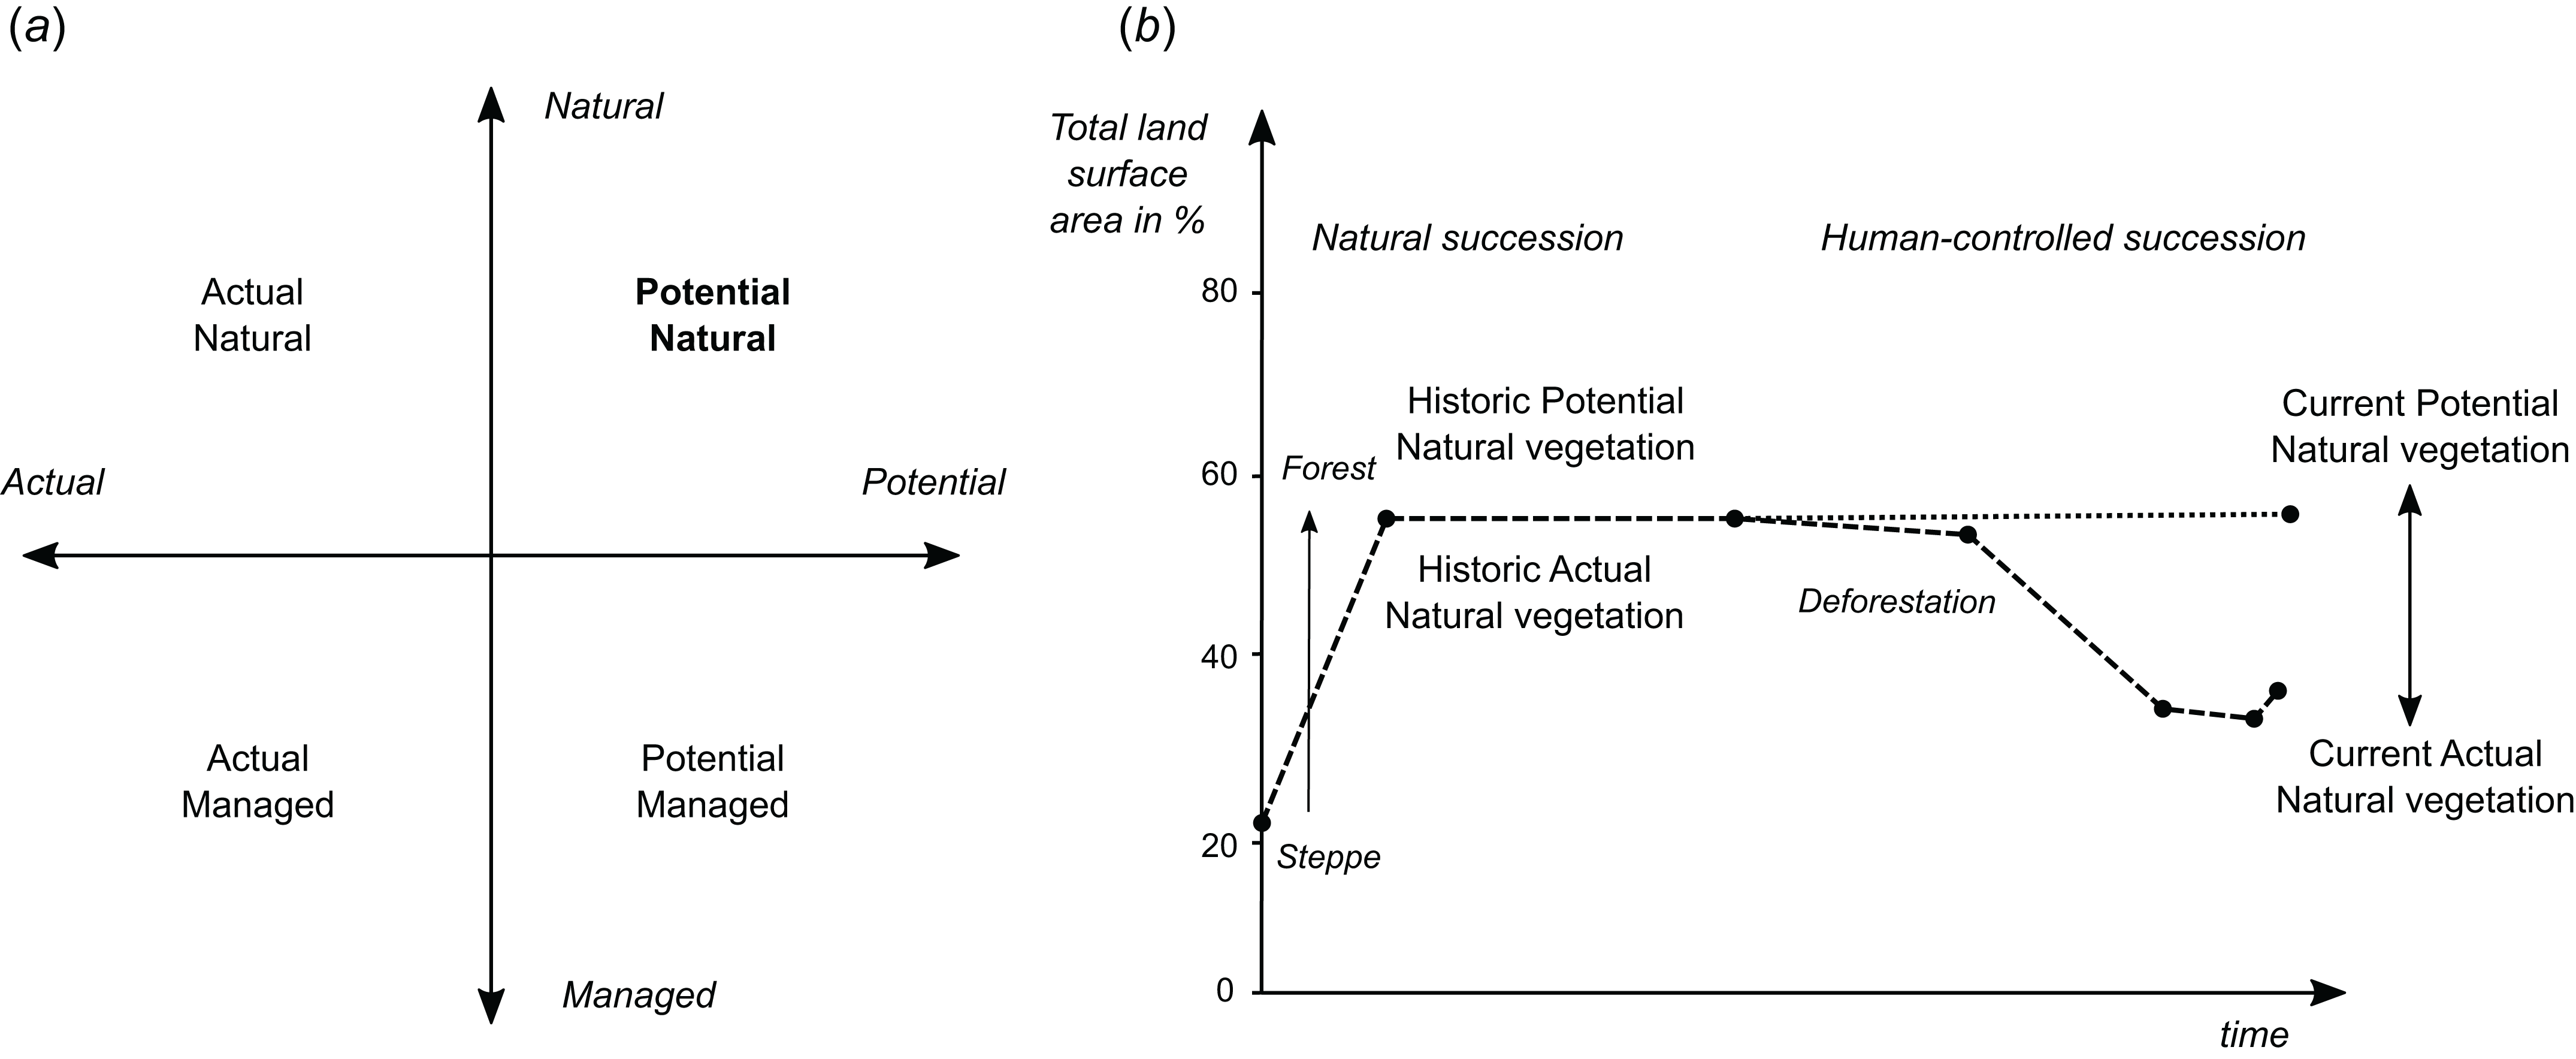
\includegraphics[width=1\linewidth]{img/fig_scheme_pnv} 

}

\caption{Schematic explanation of differences between (A) potential and actual natural/managed vegetation, and (B) current and historic vegetation in the context of global land area. Image source: https://doi.org/10.7717/peerj.5457.}\label{fig:scheme-pnv}
\end{figure}

\citet{griscom2017natural} produced the \textbf{\href{https://zenodo.org/doi/10.5281/zenodo.883443}{Global Reforestation Potential Map}} at 1-km resolution.
\citet{bastin2019global} produced \href{https://crowtherlab.com/maps/}{Potential forest cover map} at 1-km resolution assuming no humans present.
\textbf{\href{https://zenodo.org/doi/10.5281/zenodo.3631253}{Potential distribution of LCCS land cover classes}} at 250-m spatial resolution based
on the UN FAO Land Cover Classification System (LCCS) is part of the
\href{https://naturemap.earth/}{NatureMap project}. \citet{bonannella2023biomes} provides an updated
predictions of the potential distribution of \textbf{\href{https://zenodo.org/doi/10.5281/zenodo.7520813}{global biomes}} at 1-km including for the future climate scenarios (2040, 2060 and beyond).

\hypertarget{species-distribution-and-biodiversity-maps}{%
\subsection{Species distribution and biodiversity maps}\label{species-distribution-and-biodiversity-maps}}

\textbf{\href{http://data.gbif.org/}{Global Biodiversity Information Facility (GBIF)}} provides access to global data showing the distribution of
all flora and fauna species. The density maps are available only at resolution of
1 arcdegree (about 100-km) and often without any bias-correction. Global maps of biodiversity measures for various groups
of taxa (e.g.~vascular plants, birds and mammals) can be browsed using the \href{https://earthobservations.org/solutions/incubators/global-ecosystems-atlas}{Global Ecosystem Atlas}.
Similar type of maps can be browsed via the \href{http://www.unep-wcmc.org/}{UNEP's World Conservation Monitoring Centre}.

A shape file showing location of hotspot regions is distributed by the \href{http://www.biodiversityhotspots.org/}{Conservation International}.
\citet{Kreft2007} produced a \textbf{global map of plant species diversity} (number of plant species) by using
field records from 1,032 locations (maps are available only in coarse resolution of 120-km).
\href{https://datazone.birdlife.org/home}{BirdLife International} publishes a number of global maps
indicating \textbf{\href{https://datazone.birdlife.org/site/requestgis}{Endemic and Important Bird Areas}} (EBAs and IBAs).

\citet{pimm2014biodiversity} produced \textbf{\href{https://biodiversitymapping.org/}{maps of species richness}} for
mammals, birds, amphibians and other taxa at 10-km spatial resolution.
\href{https://explorer.naturemap.earth/}{EarthMap project} produced a species richness (number of species per grid cell) maps
for amphibians, birds, mammals, reptiles and a representative set of plant taxa whose
distribution overlaps in each 10-km cell, and a global map of Areas of global significance for conservation \citep{brooks2019measuring}.

\citet{sabatini2022global} produced a number of \href{https://doi.org/10.25829/idiv.3506-p4c0mo}{global biodiversity maps}
including the \textbf{map of plant species richness} at 1-km spatial resolutions. These maps are based using \href{http://www.idiv.de/splot}{sPlot database}
(whichs is available upon request by submitting a project proposal to sPlot's Steering Committee).

\hypertarget{protected-areas}{%
\subsection{Protected areas}\label{protected-areas}}

National and international protected sites and attributes can be downloaded
(ESRI Shapefiles; after registering on the website) via the \textbf{\href{http://protectedplanet.net/}{World Database On Protected Areas}}.
International Union for Conservation of Nature and Natural Resources (IUCN) has
released a Red List of Threatened Species that contains assessments for +130,000 species.
Distribution maps (presence) for these species (with limited coverage) can be downloaded from the \href{https://www.iucnredlist.org/resources/spatial-data-download}{IUCN website}.

\hypertarget{openlandmap-layers}{%
\chapter{OpenLandMap layers}\label{openlandmap-layers}}

You are reading the work-in-progress OpenLandMap.org Open Land Data Services. This chapter is currently draft version, a peer-review publication is pending. You can find the polished first edition at \url{https://openlandmap.github.io/book/}.

\hypertarget{list-of-collections}{%
\section{List of collections}\label{list-of-collections}}

\begin{Shaded}
\begin{Highlighting}[]
\NormalTok{col }\OtherTok{=} \FunctionTok{read.csv}\NormalTok{(}\StringTok{"./tabular/OpenLandMap\_tables\_collections.csv"}\NormalTok{)}
\end{Highlighting}
\end{Shaded}

\hypertarget{sentinel-5p-monthly-tropospheric-nitrogen-dioxide-density}{%
\subsection{Sentinel-5P monthly tropospheric nitrogen dioxide density}\label{sentinel-5p-monthly-tropospheric-nitrogen-dioxide-density}}

\begin{itemize}
\tightlist
\item
  🔗 URL: \url{https://stac.openlandmap.org/no2_s5p.l3.trop.tmwm/collection.json}
\item
  📰 Description: Nitrogen Dioxide Density monthly median value May 2018 -- November 2022. Derived using the \href{https://eumap.readthedocs.io}{eumap package in Python}. We derived three standard statistics: (1) 10th percentile (p10), median (m), and 90th percentile (p10).
\item
  📝 Theme: Orthoimagery
\item
  📂 DOI: \url{https://doi.org/10.5281/zenodo.7464099}
\end{itemize}

\hypertarget{sentinel-5p-long-term-tropospheric-nitrogen-dioxide-density}{%
\subsection{Sentinel-5P long-term tropospheric nitrogen dioxide density}\label{sentinel-5p-long-term-tropospheric-nitrogen-dioxide-density}}

\begin{itemize}
\tightlist
\item
  🔗 URL: \url{https://stac.openlandmap.org/no2_s5p.l3.trop.tmwm.ltm/collection.json}
\item
  📰 Description: Nitrogen Dioxide Density long term quantile from monthly median value May 2018 -- November 2022. Derived using the \href{https://eumap.readthedocs.io}{eumap package in Python}. We derived three standard statistics: (1) 10th percentile (p10), median (m), and 90th percentile (p10).
\item
  📝 Theme: Orthoimagery
\item
  📂 DOI: \url{https://doi.org/10.5281/zenodo.7464099}
\end{itemize}

\hypertarget{openlandmap-annual-soil-organic-carbon}{%
\subsection{OpenLandMap annual soil organic carbon}\label{openlandmap-annual-soil-organic-carbon}}

\begin{itemize}
\tightlist
\item
  🔗 URL: \url{https://stac.openlandmap.org/log.oc_iso.10694/collection.json}
\item
  🗞 Description: Log organic carbon {[}g/kg{]} predicted at various soil depths
\item
  📝 Theme: Geology and Soils
\item
  📂 DOI:
\end{itemize}

\hypertarget{mod13q1-long-term-enhanced-vegetation-index-evi---trend-analysis}{%
\subsection{MOD13Q1 long-term Enhanced Vegetation Index (EVI - trend analysis)}\label{mod13q1-long-term-enhanced-vegetation-index-evi---trend-analysis}}

\begin{itemize}
\tightlist
\item
  🔗 URL: \url{https://stac.openlandmap.org/evi_mod13q1.stl.trend.logit.ols.beta/collection.json}
\item
  📰 Description: Analysis-ready EVI trend component based on MOD13Q1 by every two months and fully gapfilled. The trend component was derived by \href{https://www.statsmodels.org/dev/generated/statsmodels.tsa.seasonal.STL.html\#statsmodels.tsa.seasonal.STL}{Season-Trend decomposition using LOESS}.
\item
  📝 Theme: Orthoimagery
\item
  📂 DOI:
\end{itemize}

\hypertarget{esa-cci-annual-land-cover}{%
\subsection{ESA CCI annual land cover}\label{esa-cci-annual-land-cover}}

\begin{itemize}
\tightlist
\item
  🔗 URL: \url{https://stac.openlandmap.org/land.cover_esacci.lc.l4/collection.json}
\item
  📰 Description: Based on the European Space Agency (ESA) Climate Change Initiative (ESACCI-LC).
\item
  📝 Theme: Land Cover and Land Use
\item
  📂 DOI:
\end{itemize}

\hypertarget{mod13q1-bi-monthly-enhanced-vegetation-index-index-evi}{%
\subsection{MOD13Q1 bi-monthly Enhanced Vegetation Index Index (EVI)}\label{mod13q1-bi-monthly-enhanced-vegetation-index-index-evi}}

\begin{itemize}
\tightlist
\item
  🔗 URL: \url{https://stac.openlandmap.org/evi_mod13q1.tmwm.inpaint/collection.json}
\item
  🗞 Description: Analysis-ready EVI based on MOD13Q1 aggregated by every two months, according to the percentile 90th, and fully gapfilled. The gapfilling was based in 1) \href{https://eumap.readthedocs.io/en/latest/_autosummary/eumap.gapfiller.TMWM.html\#eumap.gapfiller.TMWM}{Temporal Moving Window Median} algorithm, and 2) \href{https://eumap.readthedocs.io/en/latest/_autosummary/eumap.gapfiller.InPainting.html}{inpating} technique.
\item
  📝 Theme: Orthoimagery
\item
  📂 DOI:
\end{itemize}

\hypertarget{openlandmap-ensemble-digital-terrain-model}{%
\subsection{OpenLandMap ensemble digital terrain model}\label{openlandmap-ensemble-digital-terrain-model}}

\begin{itemize}
\tightlist
\item
  🔗 URL: \url{https://stac.openlandmap.org/dtm.bareearth_ensemble/collection.json}
\item
  📰 Description: Derived using ALOS AW3D, GLO-30, MERITDEM, and national DTMs, considering the lower 10\% quantile from all input layers. In order to create bare earth data, we used canopy height (canopy height \textgreater{} 2m) and standard deviation (sd \textgreater{} 6m) to mask building and forest in AW3D and GLO-30.
\item
  📝 Theme: Elevation and Depth
\item
  📂 DOI: \url{https://doi.org/10.5281/zenodo.7676373}
\end{itemize}

\hypertarget{monthly-fraction-of-absorbed-photosynthetically-active-radiation-fapar}{%
\subsection{Monthly fraction of absorbed photosynthetically active radiation (FAPAR)}\label{monthly-fraction-of-absorbed-photosynthetically-active-radiation-fapar}}

\begin{itemize}
\tightlist
\item
  🔗 URL: \url{https://stac.openlandmap.org/fapar_essd.lstm/collection.json}
\item
  📰 Description: The monthly aggregated Fraction of Absorbed Photosynthetically Active Radiation (FAPAR) dataset is derived from 250m 8d GLASS V6 FAPAR, considering several other FAPAR products (MODIS Collection 6, GLASS FAPAR V5, and PROBA-V1 FAPAR) to generate a bidirectional long-short-term memory (Bi-LSTM) model to adjust and harmonize FAPAR across two decades. The monthly aggregation includes three standard statistics: (1) 5th percentile (p05), median (p50), and 95th percentile (p95). For each month, we aggregate all composites within that month plus one composite each before and after, ending up with 5 to 6 composites for a single month depending on the number of images within that month.
\item
  📝 Theme: Biodiversity and Nature Conservation
\item
  📂 DOI: \url{https://doi.org/10.5281/zenodo.8408654}
\end{itemize}

\hypertarget{long-term-fraction-of-absorbed-photosynthetically-active-radiation-fapar---trend-analysis}{%
\subsection{Long-term fraction of absorbed photosynthetically active radiation (FAPAR - trend analysis)}\label{long-term-fraction-of-absorbed-photosynthetically-active-radiation-fapar---trend-analysis}}

\begin{itemize}
\tightlist
\item
  🔗 URL: \url{https://stac.openlandmap.org/fapar_essd.lstm.p95.beta/collection.json}
\item
  📰 Description: The monthly aggregated Fraction of Absorbed Photosynthetically Active Radiation (FAPAR) dataset is derived from 250m 8d GLASS V6 FAPAR, considering several other FAPAR products (MODIS Collection 6, GLASS FAPAR V5, and PROBA-V1 FAPAR) to generate a bidirectional long-short-term memory (Bi-LSTM) model to adjust and harmonize FAPAR across two decades. The trend analysis provides OLS model for the p95 time-series including: (1) slope beta mean (p95.beta\_m), p-value for beta (p95.beta\_pv), intercept alpha mean (p95.alpha\_m), p-value for alpha (p95.alpha\_pv), and coefficient of determination R2 (p95.r2\_m).
\item
  📝 Theme: Biodiversity and Nature Conservation
\item
  📂 DOI: \url{https://doi.org/10.5281/zenodo.8399173}
\end{itemize}

\hypertarget{annual-potential-fraction-of-absorbed-photosynthetically-active-radiation-fapar---2021}{%
\subsection{Annual potential fraction of absorbed photosynthetically active radiation (FAPAR - 2021)}\label{annual-potential-fraction-of-absorbed-photosynthetically-active-radiation-fapar---2021}}

\begin{itemize}
\tightlist
\item
  🔗 URL: \url{https://stac.openlandmap.org/pot.fapar_fapar.p95.eml.m/collection.json}
\item
  🗞 Description: Potential FAPAR predicted by fitting an ensemble ML model using globally distributed training points (cca 3 Mio) and a set of 52 biophysical covariates including several layers related to human pressure. The spatial layers include 1) yearly average of potential FAPAR + model deviance, 2) yearly average of FAPAR (P50).
\item
  📝 Theme: Biodiversity and Nature Conservation
\item
  📂 DOI: \url{https://doi.org/10.5281/zenodo.8404153}
\end{itemize}

\hypertarget{monthly-potential-fraction-of-absorbed-photosynthetically-active-radiation-fapar---2021}{%
\subsection{Monthly potential fraction of absorbed photosynthetically active radiation (FAPAR - 2021)}\label{monthly-potential-fraction-of-absorbed-photosynthetically-active-radiation-fapar---2021}}

\begin{itemize}
\tightlist
\item
  🔗 URL: \url{https://stac.openlandmap.org/pot.fapar_fapar.p95.eml/collection.json}
\item
  🗞 Description: Potential FAPAR predicted every month, in 2021, by fitting an ensemble ML model using globally distributed training points (cca 3 Mio) and a set of 52 biophysical covariates including several layers related to human pressure.
\item
  📝 Theme: Biodiversity and Nature Conservation
\item
  📂 DOI: \url{https://doi.org/10.5281/zenodo.8404153}
\end{itemize}

\hypertarget{esa-monthly-snow-cover-fraction}{%
\subsection{ESA monthly snow cover fraction}\label{esa-monthly-snow-cover-fraction}}

\begin{itemize}
\tightlist
\item
  🔗 URL: \url{https://stac.openlandmap.org/snow.cover_esa.modis/collection.json}
\item
  📰 Description: Global MODIS-based snow cover monthly long-term (2000-2012) at 500 m. Global snow cover monthly long-term (2000--2012) P90 and standard deviation derived from the ESA CCI snow cover weekly product.
\item
  📝 Theme: Land Cover and Land Use
\item
  📂 DOI: \url{https://doi.org/10.5281/zenodo.5774953}
\end{itemize}

\hypertarget{esa-long-term-snow-cover-fraction}{%
\subsection{ESA long-term snow cover fraction}\label{esa-long-term-snow-cover-fraction}}

\begin{itemize}
\tightlist
\item
  🔗 URL: \url{https://stac.openlandmap.org/snow.cover_esa.modis.ltm/collection.json}
\item
  📰 Description: Global MODIS-based snow cover monthly long-term (2000-2012) at 500 m. Global snow cover monthly long-term (2000--2012) P90 and standard deviation derived from the ESA CCI snow cover weekly product.
\item
  📝 Theme: Land Cover and Land Use
\item
  📂 DOI: \url{https://doi.org/10.5281/zenodo.5774953}
\end{itemize}

\hypertarget{annual-terrestrial-human-footprint}{%
\subsection{Annual terrestrial human footprint}\label{annual-terrestrial-human-footprint}}

\begin{itemize}
\tightlist
\item
  🔗 URL: \url{https://stac.openlandmap.org/wilderness_li2022.human.footprint/collection.json}
\item
  📰 Description: Dataset of annual dynamics of the global Human Footprint from 2000 to 2018 using eight variables that reflect different aspects of human pressures.
\item
  📝 Theme: Population Distribution
\item
  📂 DOI: \url{https://doi.org/10.1038/s41597-022-01284-8}
\end{itemize}

\hypertarget{mcd19a2-monthly-water-vapor}{%
\subsection{MCD19A2 monthly water vapor}\label{mcd19a2-monthly-water-vapor}}

\begin{itemize}
\tightlist
\item
  🔗 URL: \url{https://stac.openlandmap.org/wv_mcd19a2v061.seasconv/collection.json}
\item
  📰 Description: The monthly aggregated water vapor dataset is derived from MCD19A2 v061, measuring the column above ground retrieved from MODIS near-IR bands at 0.94μm. The dataset time spans from 2000 to 2022 and provides data that covers the entire globe. The monthly aggregation considered the mean and standard deviation of daily water vapor time-series data. Only positive non-cloudy pixels were considered valid observations to derive the mean and the standard deviation. The remaining no-data values were filled using the TMWM algorithm. This dataset also includes smoothed mean and standard deviation values using the Whittaker method. The quality assessment layers and the number of valid observations for each month can provide an indication of the reliability of the monthly mean and standard deviation values.
\item
  📝 Theme: Climate
\item
  📂 DOI: \url{https://doi.org/10.5281/zenodo.8226283}
\end{itemize}

\hypertarget{mcd19a2-long-term-water-vapor-perc.-50th}{%
\subsection{MCD19A2 long-term water vapor (perc. 50th)}\label{mcd19a2-long-term-water-vapor-perc.-50th}}

\begin{itemize}
\tightlist
\item
  🔗 URL: \url{https://stac.openlandmap.org/wv_mcd19a2v061.seasconv.m_p50/collection.json}
\item
  🗞 Description: The monthly aggregated water vapor dataset is derived from MCD19A2 v061, measuring the column above ground retrieved from MODIS near-IR bands at 0.94μm. The dataset time spans from 2000 to 2022 and provides data that covers the entire globe. The monthly aggregation considered the mean and standard deviation of daily water vapor time-series data. Only positive non-cloudy pixels were considered valid observations to derive the mean and the standard deviation. The remaining no-data values were filled using the TMWM algorithm. This dataset also includes smoothed mean and standard deviation values using the Whittaker method. The quality assessment layers and the number of valid observations for each month can provide an indication of the reliability of the monthly mean and standard deviation values.
\item
  📝 Theme: Climate
\item
  📂 DOI: \url{https://doi.org/10.5281/zenodo.8226283}
\end{itemize}

\hypertarget{mcd19a2-long-term-water-vapor-perc.-25th}{%
\subsection{MCD19A2 long-term water vapor (perc. 25th)}\label{mcd19a2-long-term-water-vapor-perc.-25th}}

\begin{itemize}
\tightlist
\item
  🔗 URL: \url{https://stac.openlandmap.org/wv_mcd19a2v061.seasconv.m_p25/collection.json}
\item
  📰 Description: The monthly aggregated water vapor dataset is derived from MCD19A2 v061, measuring the column above ground retrieved from MODIS near-IR bands at 0.94μm. The dataset time spans from 2000 to 2022 and provides data that covers the entire globe. The monthly aggregation considered the mean and standard deviation of daily water vapor time-series data. Only positive non-cloudy pixels were considered valid observations to derive the mean and the standard deviation. The remaining no-data values were filled using the TMWM algorithm. This dataset also includes smoothed mean and standard deviation values using the Whittaker method. The quality assessment layers and the number of valid observations for each month can provide an indication of the reliability of the monthly mean and standard deviation values.
\item
  📝 Theme: Climate
\item
  📂 DOI: \url{https://doi.org/10.5281/zenodo.8226283}
\end{itemize}

\hypertarget{mcd19a2-long-term-water-vapor-perc.-75th}{%
\subsection{MCD19A2 long-term water vapor (perc. 75th)}\label{mcd19a2-long-term-water-vapor-perc.-75th}}

\begin{itemize}
\tightlist
\item
  🔗 URL: \url{https://stac.openlandmap.org/wv_mcd19a2v061.seasconv.m_p75/collection.json}
\item
  📰 Description: The monthly aggregated water vapor dataset is derived from MCD19A2 v061, measuring the column above ground retrieved from MODIS near-IR bands at 0.94μm. The dataset time spans from 2000 to 2022 and provides data that covers the entire globe. The monthly aggregation considered the mean and standard deviation of daily water vapor time-series data. Only positive non-cloudy pixels were considered valid observations to derive the mean and the standard deviation. The remaining no-data values were filled using the TMWM algorithm. This dataset also includes smoothed mean and standard deviation values using the Whittaker method. The quality assessment layers and the number of valid observations for each month can provide an indication of the reliability of the monthly mean and standard deviation values.
\item
  📝 Theme: Climate
\item
  📂 DOI: \url{https://doi.org/10.5281/zenodo.8226283}
\end{itemize}

\hypertarget{mcd19a2-long-term-water-vapor-std.-dev.}{%
\subsection{MCD19A2 long-term water vapor (std. dev.)}\label{mcd19a2-long-term-water-vapor-std.-dev.}}

\begin{itemize}
\tightlist
\item
  🔗 URL: \url{https://stac.openlandmap.org/wv_mcd19a2v061.seasconv.m_std/collection.json}
\item
  🗞 Description: The monthly aggregated water vapor dataset is derived from MCD19A2 v061, measuring the column above ground retrieved from MODIS near-IR bands at 0.94μm. The dataset time spans from 2000 to 2022 and provides data that covers the entire globe. The monthly aggregation considered the mean and standard deviation of daily water vapor time-series data. Only positive non-cloudy pixels were considered valid observations to derive the mean and the standard deviation. The remaining no-data values were filled using the TMWM algorithm. This dataset also includes smoothed mean and standard deviation values using the Whittaker method. The quality assessment layers and the number of valid observations for each month can provide an indication of the reliability of the monthly mean and standard deviation values.
\item
  📝 Theme: Climate
\item
  📂 DOI: \url{https://doi.org/10.5281/zenodo.8226283}
\end{itemize}

\hypertarget{mcd19a2-annual-water-vapor}{%
\subsection{MCD19A2 annual water vapor}\label{mcd19a2-annual-water-vapor}}

\begin{itemize}
\tightlist
\item
  🔗 URL: \url{https://stac.openlandmap.org/wv_mcd19a2v061.seasconv.m.yearly/collection.json}
\item
  🗞 Description: The monthly aggregated water vapor dataset is derived from MCD19A2 v061, measuring the column above ground retrieved from MODIS near-IR bands at 0.94μm. The dataset time spans from 2000 to 2022 and provides data that covers the entire globe. The monthly aggregation considered the mean and standard deviation of daily water vapor time-series data. Only positive non-cloudy pixels were considered valid observations to derive the mean and the standard deviation. The remaining no-data values were filled using the TMWM algorithm. This dataset is specifically derived from monthly time-series, providing a yearly time-series aggregated statistics of the monthly time-series data.
\item
  📝 Theme: Climate
\item
  📂 DOI: \url{https://doi.org/10.5281/zenodo.8226282}
\end{itemize}

\hypertarget{long-term-soil-bulk-density-for-fine-earth}{%
\subsection{Long-term soil bulk density for fine earth}\label{long-term-soil-bulk-density-for-fine-earth}}

\begin{itemize}
\tightlist
\item
  🔗 URL: \url{https://stac.openlandmap.org/bulkdens.fineearth_usda.4a1h/collection.json}
\item
  📰 Description: Soil bulk density (fine earth) 10 x kg / m-cubic at 6 standard depths (0, 10, 30, 60, 100 and 200 cm) at 250 m resolution
\item
  📝 Theme: Geology and Soils
\item
  📂 DOI: \url{https://doi.org/10.5281/zenodo.2525665}
\end{itemize}

\hypertarget{merit-geomorphometry}{%
\subsection{MERIT geomorphometry}\label{merit-geomorphometry}}

\begin{itemize}
\tightlist
\item
  🔗 URL: \url{https://stac.openlandmap.org/geom_merit.dem/collection.json}
\item
  📰 Description: Relief parameters were derived derived using SAGA GIS (\url{http://www.saga-gis.org/}) and the MERIT DEM (Yamazaki et al.~2017) projected in the Equi7 grid system (Bauer-Marschallinger et al.~2014). Once derived, DEM derivatives were then reprojected to the lon-lat system.
\item
  📝 Theme: Geology and Soils
\item
  📂 DOI: \url{https://doi.org/10.1038/s41597-020-0479-6}
\end{itemize}

\hypertarget{proba-v-long-term-fraction-of-absorbed-photosynthetically-active-radiation-fapar}{%
\subsection{PROBA-V long-term fraction of absorbed photosynthetically active radiation (FAPAR)}\label{proba-v-long-term-fraction-of-absorbed-photosynthetically-active-radiation-fapar}}

\begin{itemize}
\tightlist
\item
  🔗 URL: \url{https://stac.openlandmap.org/fapar_proba.v/collection.json}
\item
  🗞 Description: Fraction of absorbed photosynthetically active radiation monthly images for 2014--2017 were obtained from \url{https://land.copernicus.eu} (original values reported in the range 0--235 with scaling factor 1/255, i.e., with a maximum value of 0.94). From a total of 142 images downloaded from \url{https://land.copernicus.eu} we derived minimum, median and maximum value of FAPAR per month (12) using the 95\% probability interval using the data.table package (\url{http://r-datatable.com}).
\item
  📝 Theme: Orthoimagery
\item
  📂 DOI: \url{https://doi.org/10.5281/zenodo.3459830}
\end{itemize}

\hypertarget{tree-covered-and-intact-forest-landscapes}{%
\subsection{Tree-covered and intact forest landscapes}\label{tree-covered-and-intact-forest-landscapes}}

\begin{itemize}
\tightlist
\item
  🔗 URL: \url{https://stac.openlandmap.org/forest.cover_esacci.ifl/collection.json}
\item
  📰 Description: Based on the UNEP historic forest cover map, ESA land cover time series and intact forest landscape (IFL 2000, 2013 and 2016) data (Potapov et al.~2013).
\item
  📝 Theme: Land Cover and Land Use
\item
  📂 DOI: \url{https://doi.org/10.5281/zenodo.1477073}
\end{itemize}

\hypertarget{usda-long-term-soil-great-groups}{%
\subsection{USDA long-term soil great groups}\label{usda-long-term-soil-great-groups}}

\begin{itemize}
\tightlist
\item
  🔗 URL: \url{https://stac.openlandmap.org/grtgroup_usda.soiltax/collection.json}
\item
  📰 Description: Distribution of the USDA soil great groups based on machine learning predictions from global compilation of soil profiles (\textgreater350,000 training points).
\item
  📝 Theme: Geology and Soils
\item
  📂 DOI: \url{https://doi.org/10.5281/zenodo.3528062}
\end{itemize}

\hypertarget{copernicus-proba-v-annual-land-cover}{%
\subsection{Copernicus PROBA-V annual land cover}\label{copernicus-proba-v-annual-land-cover}}

\begin{itemize}
\tightlist
\item
  🔗 URL: \url{https://stac.openlandmap.org/land.cover_copernicus/collection.json}
\item
  📰 Description: Annual, global 100m land cover maps in 2015, 2016, 2017, 2018, 2019, produced by the global component of the Copernicus Land Service, derived from PROBA-V satellite observations and ancillary datasets
\item
  📝 Theme: Land Cover and Land Use
\item
  📂 DOI: \url{https://doi.org/10.5281/zenodo.4723924}
\end{itemize}

\hypertarget{openlandmap-long-term-soil-organic-carbon-stock}{%
\subsection{OpenLandMap long-term soil organic carbon stock}\label{openlandmap-long-term-soil-organic-carbon-stock}}

\begin{itemize}
\tightlist
\item
  🔗 URL: \url{https://stac.openlandmap.org/organic.carbon.stock_msa.kgm2/collection.json}
\item
  🗞 Description: Soil organic carbon stock in kg/m2 for 5 standard depth intervals (0--10, 10--30, 30--60, 60--100 and 100--200 cm) at 250 m resolution. To convert to t/ha multiply by 10. Derived using soil organic carbon content (\url{https://doi.org/10.5281/zenodo.1475457}), bulk density (\url{https://doi.org/10.5281/zenodo.1475970}) and coarse fragments (\url{https://doi.org/10.5281/zenodo.2525681}), predicted from point data at 6 standard depths. Depth to bed rock has been ignored, hence total stocks might be about 10--15\% lower then reported.
\item
  📝 Theme: Geology and Soils
\item
  📂 DOI: \url{https://doi.org/10.5281/zenodo.2536040}
\end{itemize}

\hypertarget{openlandmap-long-term-soil-organic-carbon-content}{%
\subsection{OpenLandMap long-term soil organic carbon content}\label{openlandmap-long-term-soil-organic-carbon-content}}

\begin{itemize}
\tightlist
\item
  🔗 URL: \url{https://stac.openlandmap.org/organic.carbon_usda.6a1c/collection.json}
\item
  📰 Description: Soil organic carbon content in x 5 g / kg (to convert to \% divide by 2) at 6 standard depths (0, 10, 30, 60, 100 and 200 cm) at 250 m resolution.Predicted from a global compilation of soil points. Also available for download: soil organic stock maps in in kg / m2 (\url{https://doi.org/10.5281/zenodo.1475453}) and bulk density maps in kg / m3 (\url{https://doi.org/10.5281/zenodo.1475970}).
\item
  📝 Theme: Geology and Soils
\item
  📂 DOI: \url{https://doi.org/10.5281/zenodo.2525553}
\end{itemize}

\hypertarget{esa-cci-annual-plant-functional-types-pft}{%
\subsection{ESA CCI annual plant functional types (PFT)}\label{esa-cci-annual-plant-functional-types-pft}}

\begin{itemize}
\tightlist
\item
  🔗 URL: \url{https://stac.openlandmap.org/pft.landcover_esa.cci.lc/collection.json}
\item
  🗞 Description: This dataset contains Global Plant Functional Types (PFT) data, from the ESA Medium Resolution Land Cover (MRLC) Climate Change Initiative project. The data provides yearly data, and initially covers the time period from 1992 to 2020. It is anticipated that the dataset will be updated annually going forward. The PFT v2.0.8 global dataset has 14 layers, each describing the percentage cover (0-100\%) of a plant functional type at a spatial resolution of 300 m: broadleaved evergreen trees, broadleaved deciduous trees, needleleaved evergreen trees, needleleaved deciduous trees, broadleaved evergreen shrubs, broadleaved deciduous shrubs, needleleaved evergreen shrubs, needleleaved deciduous shrubs, natural grasses, herbaceous cropland (i.e., managed grasses), built, water, bare areas, and snow and ice.
\item
  📝 Theme: Land Cover and Land Use
\item
  📂 DOI: \url{https://doi.org/10.5285/26a0f46c95ee4c29b5c650b129aab788}
\end{itemize}

\hypertarget{sm2rain-long-term-precipitation}{%
\subsection{SM2RAIN long-term precipitation}\label{sm2rain-long-term-precipitation}}

\begin{itemize}
\tightlist
\item
  🔗 URL: \url{https://stac.openlandmap.org/precipitation_sm2rain.ltm/collection.json}
\item
  🗞 Description: Monthly precipitation in mm at 1 km resolution based on SM2RAIN-ASCAT 2007-2021 (\url{https://doi.org/10.5281/zenodo.2615278}). Downscaled to 1 km resolution using gdalwarp (cubic splines) and combined with WorldClim (\url{https://worldclim.org/data/worldclim21.html}) and CHELSA Climate (\url{https://chelsa-climate.org/downloads/}) monthly values. Final values are estimated as a simple average between the three precipitation data sources; a more objective approach would be to use training points e.g.~meteo-station monthly values, then train an ensemble model using the 3 data sources as independent variables. Another global data source of precipitation images is the monthly IMERGE dataset, however this requires transformation and is available only for limited span of years.
\item
  📝 Theme: Climate
\item
  📂 DOI: \url{https://doi.org/10.5281/zenodo.6458580}
\end{itemize}

\hypertarget{openlandmap-long-term-soil-ph}{%
\subsection{OpenLandMap long-term soil pH}\label{openlandmap-long-term-soil-ph}}

\begin{itemize}
\tightlist
\item
  🔗 URL: \url{https://stac.openlandmap.org/ph.h2o_usda.4c1a2a/collection.json}
\item
  📰 Description: Soil pH in H2O at 6 standard depths (0, 10, 30, 60, 100 and 200 cm) at 250 m resolution according to USDA method code: 4C1a2a
\item
  📝 Theme: Geology and Soils
\item
  📂 DOI: \url{https://doi.org/10.5281/zenodo.2525664}
\end{itemize}

\hypertarget{jrc-global-human-settlement-annual-population-ghs}{%
\subsection{JRC Global Human Settlement annual population (GHS)}\label{jrc-global-human-settlement-annual-population-ghs}}

\begin{itemize}
\tightlist
\item
  🔗 URL: \url{https://stac.openlandmap.org/pop.count_ghs.jrc/collection.json}
\item
  📰 Description: This GHS-POP spatial raster product (GHS-POP\_GLOBE\_R2023) depicts the distribution of human population, expressed as the number of people per cell. Residential population estimates at 5 years interval between 1975 and 2030 are derived from the raw global census data harmonized by CIESIN for the Gridded Population of the World, version 4.11 (GPWv4.11) at polygon level, and disaggregated from census or administrative units to grid cells, informed by the distribution, classification and volume of built-up as mapped in the GHSL global layers per corresponding epoch. The disaggregation methodology is described in Freire et al., (2016).
\item
  📝 Theme: Population Distribution
\item
  📂 DOI: \url{https://doi.org/10.2905/2FF68A52-5B5B-4A22-8F40-C41DA8332CFE}
\end{itemize}

\hypertarget{openlandmap-long-term-sand-content}{%
\subsection{OpenLandMap long-term sand content}\label{openlandmap-long-term-sand-content}}

\begin{itemize}
\tightlist
\item
  🔗 URL: \url{https://stac.openlandmap.org/sand.wfraction_usda.3a1a1a/collection.json}
\item
  🗞 Description: Sand content in \% (kg / kg) at 6 standard depths (0, 10, 30, 60, 100 and 200 cm) at 250 m resolution. Based on machine learning predictions from global compilation of soil profiles and samples.
\item
  📝 Theme: Water
\item
  📂 DOI: \url{https://doi.org/10.5281/zenodo.2525662}
\end{itemize}

\hypertarget{mcd12q1-annual-land-cover-and-land-use}{%
\subsection{MCD12Q1 annual land cover and land use}\label{mcd12q1-annual-land-cover-and-land-use}}

\begin{itemize}
\tightlist
\item
  🔗 URL: \url{https://stac.openlandmap.org/lc_mcd12q1v061.p1/collection.json}
\item
  🗞 Description: The yearly land use and land cover dataset is derived from MCD12Q1 v061. This data provides an yearly mosaics of land use and land cover data from 2001 to 2022. This dataset includes layers of land cover type 1 (t1), 2 (t2), and 5 (t5), land cover property 1 (p1) and 2 (p2), land cover property assessment 1 (p1a) and 2 (p2a), and land cover quality control (qc).
\item
  📝 Theme: Land Cover and Land Use
\item
  📂 DOI: \url{https://doi.org/10.5281/zenodo.8367523}
\end{itemize}

\hypertarget{openlandmap-long-term-soil-texture-classes-usda-system}{%
\subsection{OpenLandMap long-term soil texture classes (USDA system)}\label{openlandmap-long-term-soil-texture-classes-usda-system}}

\begin{itemize}
\tightlist
\item
  🔗 URL: \url{https://stac.openlandmap.org/texture.class_usda.tt/collection.json}
\item
  🗞 Description: Soil texture classes (USDA system) for 6 standard soil depths (0, 10, 30, 60, 100 and 200 cm) at 250 m.
\item
  📝 Theme: Geology and Soils
\item
  📂 DOI: \url{https://doi.org/10.5281/zenodo.2525817}
\end{itemize}

\hypertarget{jrc-long-term-surface-water-occurrence}{%
\subsection{JRC long-term surface water occurrence}\label{jrc-long-term-surface-water-occurrence}}

\begin{itemize}
\tightlist
\item
  🔗 URL: \url{https://stac.openlandmap.org/water.occurrence_jrc.surfacewater/collection.json}
\item
  📰 Description: Gobal surface water occurrence based on Pekel at al.~(2016), and the layer is resampled to spatial resolution 1/480 d.d. (about 250 m) using gdalwarp with ``average'' resampling. Original layers are available at 30 m resolution. The orignal dataset and document: \url{https://doi.org/10.1038/nature20584}.
\item
  📝 Theme: Water
\item
  📂 DOI: \url{https://doi.org/10.5281/zenodo.1439254}
\end{itemize}

\hypertarget{openlandmap-long-term-soil-water-content}{%
\subsection{OpenLandMap long-term soil water content}\label{openlandmap-long-term-soil-water-content}}

\begin{itemize}
\tightlist
\item
  🔗 URL: \url{https://stac.openlandmap.org/watercontent.33kPa_usda.4b1c/collection.json}
\item
  📰 Description: Soil water content (volumetric) in percent for 33 kPa and 1500 kPa suctions predicted at 6 standard depths (0, 10, 30, 60, 100 and 200 cm) at 250 m resolution. Training points are based on a global compilation of soil profiles (USDA NCSS, AfSPDB, ISRIC WISE, EGRPR, SPADE, CanNPDB, UNSODA, SWIG, HYBRAS and HydroS). Data import steps are available here. Spatial prediction steps are described in detail here. Note: these are actually measured and mapped soil content values; no Pedo-Transfer-Functions have been used (except to fill-in the missing NCSS bulk densities). Available water capacity in mm (derived as a difference between field capacity and wilting point multiplied by layer thickness) per layer is available here. Antarctica is not included.
\item
  📝 Theme: Geology and Soils
\item
  📂 DOI: \url{https://doi.org/10.5281/zenodo.2784001}
\end{itemize}

\hypertarget{copernius-dem-digital-surface-model}{%
\subsection{Copernius DEM digital surface model}\label{copernius-dem-digital-surface-model}}

\begin{itemize}
\tightlist
\item
  🔗 URL: \url{https://stac.openlandmap.org/dsm_glo30/collection.json}
\item
  🗞 Description: Global mosaic of 30m Copernicus DEM. The Copernicus DEM is a Digital Surface Model (DSM) that represents the surface of the Earth including buildings, infrastructure and vegetation. Data were acquired through the TanDEM-X mission between 2011 and 2015.
\item
  📝 Theme: Elevation and Depth
\item
  📂 DOI: \url{https://doi.org/10.5270/ESA-c5d3d65}
\end{itemize}

\hypertarget{umd-glad-annual-land-cover-and-land-use-glcluc}{%
\subsection{UMD GLAD annual land cover and land use (GLCLUC)}\label{umd-glad-annual-land-cover-and-land-use-glcluc}}

\begin{itemize}
\tightlist
\item
  🔗 URL: \url{https://stac.openlandmap.org/lc_glad.glcluc/collection.json}
\item
  📰 Description: The global 30-m spatial resolution dataset quantifies changes in forest extent and height, cropland, built-up lands, surface water, and perennial snow and ice extent from the year 2000 to 2020. Landsat Analysis Ready Data served as an input for land cover and use mapping. Each thematic product was independently derived using locally and regionally calibrated machine learning tools.
\item
  📝 Theme: Land Cover and Land Use
\item
  📂 DOI: \url{https://doi.org/10.3389/frsen.2022.856903}
\end{itemize}

\hypertarget{umd-glad-annual-land-cover-and-land-use-change-glcluc}{%
\subsection{UMD GLAD annual land cover and land use change (GLCLUC)}\label{umd-glad-annual-land-cover-and-land-use-change-glcluc}}

\begin{itemize}
\tightlist
\item
  🔗 URL: \url{https://stac.openlandmap.org/lc_glad.glcluc.change/collection.json}
\item
  📰 Description: The global 30-m spatial resolution dataset quantifies changes in forest extent and height, cropland, built-up lands, surface water, and perennial snow and ice extent from the year 2000 to 2020. Landsat Analysis Ready Data served as an input for land cover and use mapping. Each thematic product was independently derived using locally and regionally calibrated machine learning tools.
\item
  📝 Theme: Land Cover and Land Use
\item
  📂 DOI: \url{https://doi.org/10.3389/frsen.2022.856903}
\end{itemize}

\hypertarget{hyde-annual-cropland-for-the-holocene}{%
\subsection{HYDE annual cropland for the holocene}\label{hyde-annual-cropland-for-the-holocene}}

\begin{itemize}
\tightlist
\item
  🔗 URL: \url{https://stac.openlandmap.org/landuse.cropland_hyde/collection.json}
\item
  🗞 Description: History Database of the Global Environment (HYDE version 3.2). HYDE is an internally consistent combination of historical population estimates and allocation algorithms with time-dependent weighting maps for land use.
\item
  📝 Theme: Land Cover and Land Use
\item
  📂 DOI: \url{https://doi.org/10.17026/dans-25g-gez3}
\end{itemize}

\hypertarget{hyde-annual-pasture-for-the-holocene}{%
\subsection{HYDE annual pasture for the holocene}\label{hyde-annual-pasture-for-the-holocene}}

\begin{itemize}
\tightlist
\item
  🔗 URL: \url{https://stac.openlandmap.org/landuse.pasture_hyde/collection.json}
\item
  📰 Description: History Database of the Global Environment (HYDE version 3.2). HYDE is an internally consistent combination of historical population estimates and allocation algorithms with time-dependent weighting maps for land use.
\item
  📝 Theme: Land Cover and Land Use
\item
  📂 DOI: \url{https://doi.org/10.17026/dans-25g-gez3}
\end{itemize}

\hypertarget{hilda-annual-land-use-and-land-cover-change}{%
\subsection{HILDA+ annual land use and land cover change}\label{hilda-annual-land-use-and-land-cover-change}}

\begin{itemize}
\tightlist
\item
  🔗 URL: \url{https://stac.openlandmap.org/land.use.land.cover_hilda.plus/collection.json}
\item
  🗞 Description: HILDA+ (HIstoric Land Dynamics Assessment+) global dataset indicates annual land use/cover change between 1960-2019 at 1 km spatial resolution. It integrates multiple open data streams (from high-resolution remote sensing, long-term land use reconstructions and statistics). It covers six generic land use/cover categories: 1: Urban areas, 2: Cropland, 3: Pasture/rangeland, 4: Forest, 5: Unmanaged grass/shrubland, 6: Sparse/no vegetation.
\item
  📝 Theme: Land Cover and Land Use
\item
  📂 DOI: \url{https://doi.org/10.1594/PANGAEA.921846}
\end{itemize}

\hypertarget{mod11a2-long-term-land-surface-temperature-trend-daytime}{%
\subsection{MOD11A2 long-term land surface temperature trend (daytime)}\label{mod11a2-long-term-land-surface-temperature-trend-daytime}}

\begin{itemize}
\tightlist
\item
  🔗 URL: \url{https://stac.openlandmap.org/lst_mod11a2.daytime.trend.logit.ols.beta/collection.json}
\item
  📰 Description: Long-term trend analysis of MOD11A2 monthly LST day-time temperatures. Trend was produced by fitting regression models to de-seasonalized time-series. Models are fitted for each pixel and several long-term temporal metrics (alpha, beta, P\textgreater\textbar t\textbar, rsqr) has been derived.
\item
  📝 Theme: Climate
\item
  📂 DOI: \url{https://doi.org/10.5281/zenodo.1420114}
\end{itemize}

\hypertarget{mod11a2-long-term-land-surface-temperature-trend-nighttime}{%
\subsection{MOD11A2 long-term land surface temperature trend (nighttime)}\label{mod11a2-long-term-land-surface-temperature-trend-nighttime}}

\begin{itemize}
\tightlist
\item
  🔗 URL: \url{https://stac.openlandmap.org/lst_mod11a2.nighttime.trend.logit.ols.beta/collection.json}
\item
  🗞 Description: Long-term trend analysis of MOD11A2 monthly LST night-time temperatures. Trend was produced by fitting regression models to de-seasonalized time-series. Models are fitted for each pixel and several long-term temporal metrics (alpha, beta, P\textgreater\textbar t\textbar, rsqr) has been derived.
\item
  📝 Theme: Climate
\item
  📂 DOI: \url{https://doi.org/10.5281/zenodo.1420114}
\end{itemize}

\hypertarget{mod11a2-annual-land-surface-temperature-day-time}{%
\subsection{MOD11A2 annual land surface temperature (day-time)}\label{mod11a2-annual-land-surface-temperature-day-time}}

\begin{itemize}
\tightlist
\item
  🔗 URL: \url{https://stac.openlandmap.org/lst_mod11a2.daytime.annual/collection.json}
\item
  📰 Description: Day-time land surface temperature, derived from MOD11A2, yearly aggregated considering three percentiles (p05, p50 and p95) and standard deviation of cloud-free pixels. All months were gapfilled by TMWM, which uses cloud-free pixel values from diferent periods to interpolate the missing values.
\item
  📝 Theme: Climate
\item
  📂 DOI: \url{https://doi.org/10.5281/zenodo.1420114}
\end{itemize}

\hypertarget{mod11a2-annual-land-surface-temperature-night-time}{%
\subsection{MOD11A2 annual land surface temperature (night-time)}\label{mod11a2-annual-land-surface-temperature-night-time}}

\begin{itemize}
\tightlist
\item
  🔗 URL: \url{https://stac.openlandmap.org/lst_mod11a2.nighttime.annual/collection.json}
\item
  🗞 Description: Night-time land surface temperature, derived from MOD11A2, yearly aggregated considering three percentiles (p05, p50 and p95) and standard deviation of cloud-free pixels. All months were gapfilled by TMWM, which uses cloud-free pixel values from diferent periods to interpolate the missing values.
\item
  📝 Theme: Climate
\item
  📂 DOI: \url{https://doi.org/10.5281/zenodo.1420114}
\end{itemize}

\hypertarget{mod11a2-monthly-land-surface-temperature-day-time}{%
\subsection{MOD11A2 monthly land surface temperature (day-time)}\label{mod11a2-monthly-land-surface-temperature-day-time}}

\begin{itemize}
\tightlist
\item
  🔗 URL: \url{https://stac.openlandmap.org/lst_mod11a2.daytime/collection.json}
\item
  🗞 Description: Day-time land surface temperature, derived from MOD11A2, monthly aggregated considering three percentiles (p05, p50 and p95) and standard deviation of cloud-free pixels. All months were gapfilled by TMWM, which uses cloud-free pixel values from diferent periods to interpolate the missing values.
\item
  📝 Theme: Climate
\item
  📂 DOI: \url{https://doi.org/10.5281/zenodo.1420114}
\end{itemize}

\hypertarget{mod11a2-monthly-land-surface-temperature-night-time}{%
\subsection{MOD11A2 monthly land surface temperature (night-time)}\label{mod11a2-monthly-land-surface-temperature-night-time}}

\begin{itemize}
\tightlist
\item
  🔗 URL: \url{https://stac.openlandmap.org/lst_mod11a2.nighttime/collection.json}
\item
  📰 Description: Night-time land surface temperature, derived from MOD11A2, monthly aggregated considering three percentiles (p05, p50 and p95) and standard deviation of cloud-free pixels. All months were gapfilled by TMWM, which uses cloud-free pixel values from diferent periods to interpolate the missing values.
\item
  📝 Theme: Climate
\item
  📂 DOI: \url{https://doi.org/10.5281/zenodo.1420114}
\end{itemize}

\hypertarget{openlandmap-landform-classes}{%
\subsection{OpenLandMap landform classes}\label{openlandmap-landform-classes}}

\begin{itemize}
\tightlist
\item
  🔗 URL: \url{https://stac.openlandmap.org/landform_usgs.ecotapestry/collection.json}
\item
  🗞 Description: Layers include: landform (7) indicator maps (0-100\%). Derived from the USGS Global Ecosystem Map, i.e.~the EcoTapestry map. Water bodies masked out. Antarctica is not included.
\item
  📝 Theme: Geology and Soils
\item
  📂 DOI: \url{https://doi.org/10.5281/zenodo.1464846}
\end{itemize}

\hypertarget{openlandmap-lithology-classes}{%
\subsection{OpenLandMap lithology classes}\label{openlandmap-lithology-classes}}

\begin{itemize}
\tightlist
\item
  🔗 URL: \url{https://stac.openlandmap.org/lithology_usgs.ecotapestry/collection.json}
\item
  📰 Description: Layers include: lithology (15) indicator maps (0-100\%). Derived from the USGS Global Ecosystem Map, i.e.~the EcoTapestry map. Water bodies masked out. Antarctica is not included.
\item
  📝 Theme: Geology and Soils
\item
  📂 DOI: \url{https://doi.org/10.5281/zenodo.1464846}
\end{itemize}

\hypertarget{openlandmap-haopludalfs-of-usda-soil-great-groups}{%
\subsection{OpenLandMap Haopludalfs of USDA soil great groups}\label{openlandmap-haopludalfs-of-usda-soil-great-groups}}

\begin{itemize}
\tightlist
\item
  🔗 URL: \url{https://stac.openlandmap.org/grtgroup_usda.soiltax.hapludalfs/collection.json}
\item
  🗞 Description: Distribution of hapludalfs ofthe USDA soil great groups based on machine learning predictions from global compilation of soil profiles (\textgreater350,000 training points).
\item
  📝 Theme: Geology and Soils
\item
  📂 DOI: \url{https://doi.org/10.5281/zenodo.3528062}
\end{itemize}

\hypertarget{potential-distribution-of-biomes}{%
\subsection{Potential distribution of biomes}\label{potential-distribution-of-biomes}}

\begin{itemize}
\tightlist
\item
  🔗 URL: \url{https://stac.openlandmap.org/biome.type_biome00k/collection.json}
\item
  🗞 Description: Potential distribution of biomes (Potential Natural Vegetation) at 250 m spatial resolution based on the BIOME 6000 data set (8057 modern pollen-based site reconstructions). Predicted at 250 m using Ensemble Machine Learning and relief and climate variables representing the climate for the last 20+ years.
\item
  📝 Theme: Biodiversity and Nature Conservation
\item
  📂 DOI: \url{https://doi.org/10.5281/zenodo.3526620}
\end{itemize}

\hypertarget{potential-distribution-of-tropical-evergreen-broadleaf-forest}{%
\subsection{Potential distribution of tropical evergreen broadleaf forest}\label{potential-distribution-of-tropical-evergreen-broadleaf-forest}}

\begin{itemize}
\tightlist
\item
  🔗 URL: \url{https://stac.openlandmap.org/biomes_biome6k.tropical.evergreen.broadleaf.forest/collection.json}
\item
  🗞 Description: Probability and uncertainty maps showing the potential current natural vegetation (tropical evergreen broadleaf forest) on a global scale. Current (2022 - 2023) conditions are calculated on historical long term averages (1979 - 2013)
\item
  📝 Theme: Biodiversity and Nature Conservation
\item
  📂 DOI: \url{https://doi.org/10.5281/zenodo.7822868}
\end{itemize}

\hypertarget{future-potential-distribution-of-tropical-evergreen-broadleaf-forest-rcp-2.6}{%
\subsection{Future potential distribution of tropical evergreen broadleaf forest (RCP 2.6)}\label{future-potential-distribution-of-tropical-evergreen-broadleaf-forest-rcp-2.6}}

\begin{itemize}
\tightlist
\item
  🔗 URL: \url{https://stac.openlandmap.org/biomes_biome6k.tropical.evergreen.broadleaf.forest.rcp26/collection.json}
\item
  📰 Description: Probability and uncertainty maps showing the potential future natural vegetation (tropical evergreen broadleaf forest) on a global scale. Future projections (RCP 2.6) cover two different epochs: 2041 - 2060 and 2061 - 2080
\item
  📝 Theme: Biodiversity and Nature Conservation
\item
  📂 DOI: \url{https://doi.org/10.5281/zenodo.7822868}
\end{itemize}

\hypertarget{future-potential-distribution-of-tropical-evergreen-broadleaf-forest-rcp-4.5}{%
\subsection{Future potential distribution of tropical evergreen broadleaf forest (RCP 4.5)}\label{future-potential-distribution-of-tropical-evergreen-broadleaf-forest-rcp-4.5}}

\begin{itemize}
\tightlist
\item
  🔗 URL: \url{https://stac.openlandmap.org/biomes_biome6k.tropical.evergreen.broadleaf.forest.rcp45/collection.json}
\item
  📰 Description: Probability and uncertainty maps showing the potential future natural vegetation (tropical evergreen broadleaf forest) on a global scale. Future projections (RCP 4.5) cover two different epochs: 2041 - 2060 and 2061 - 2080
\item
  📝 Theme: Biodiversity and Nature Conservation
\item
  📂 DOI: \url{https://doi.org/10.5281/zenodo.7822868}
\end{itemize}

\hypertarget{future-potential-distribution-of-tropical-evergreen-broadleaf-forest-rcp-8.5}{%
\subsection{Future potential distribution of tropical evergreen broadleaf forest (RCP 8.5)}\label{future-potential-distribution-of-tropical-evergreen-broadleaf-forest-rcp-8.5}}

\begin{itemize}
\tightlist
\item
  🔗 URL: \url{https://stac.openlandmap.org/biomes_biome6k.tropical.evergreen.broadleaf.forest.rcp85/collection.json}
\item
  🗞 Description: Probability and uncertainty maps showing the potential future natural vegetation (tropical evergreen broadleaf forest) on a global scale. Future projections (RCP 8.5) cover two different epochs: 2041 - 2060 and 2061 - 2080
\item
  📝 Theme: Biodiversity and Nature Conservation
\item
  📂 DOI: \url{https://doi.org/10.5281/zenodo.7822868}
\end{itemize}

\hypertarget{potential-distribution-of-tropical-savanna}{%
\subsection{Potential distribution of tropical savanna}\label{potential-distribution-of-tropical-savanna}}

\begin{itemize}
\tightlist
\item
  🔗 URL: \url{https://stac.openlandmap.org/biomes_biome6k.tropical.savanna/collection.json}
\item
  🗞 Description: Probability and uncertainty maps showing the potential current natural vegetation (tropical savanna) on a global scale. Current (2022 - 2023) conditions are calculated on historical long term averages (1979 - 2013)
\item
  📝 Theme: Biodiversity and Nature Conservation
\item
  📂 DOI: \url{https://doi.org/10.5281/zenodo.7822868}
\end{itemize}

\hypertarget{future-potential-distribution-of-tropical-savanna-rcp-2.6}{%
\subsection{Future potential distribution of tropical savanna (RCP 2.6)}\label{future-potential-distribution-of-tropical-savanna-rcp-2.6}}

\begin{itemize}
\tightlist
\item
  🔗 URL: \url{https://stac.openlandmap.org/biomes_biome6k.tropical.savanna.rcp26/collection.json}
\item
  📰 Description: Probability and uncertainty maps showing the potential future natural vegetation (tropical savanna) on a global scale. Future projections (RCP 2.6) cover two different epochs: 2041 - 2060 and 2061 - 2080
\item
  📝 Theme: Biodiversity and Nature Conservation
\item
  📂 DOI: \url{https://doi.org/10.5281/zenodo.7822868}
\end{itemize}

\hypertarget{future-potential-distribution-of-tropical-savanna-rcp-4.5}{%
\subsection{Future potential distribution of tropical savanna (RCP 4.5)}\label{future-potential-distribution-of-tropical-savanna-rcp-4.5}}

\begin{itemize}
\tightlist
\item
  🔗 URL: \url{https://stac.openlandmap.org/biomes_biome6k.tropical.savanna.rcp45/collection.json}
\item
  🗞 Description: Probability and uncertainty maps showing the potential future natural vegetation (tropical savanna) on a global scale. Future projections (RCP 4.5) cover two different epochs: 2041 - 2060 and 2061 - 2080
\item
  📝 Theme: Biodiversity and Nature Conservation
\item
  📂 DOI: \url{https://doi.org/10.5281/zenodo.7822868}
\end{itemize}

\hypertarget{future-potential-distribution-of-tropical-savanna-rcp-8.5}{%
\subsection{Future potential distribution of tropical savanna (RCP 8.5)}\label{future-potential-distribution-of-tropical-savanna-rcp-8.5}}

\begin{itemize}
\tightlist
\item
  🔗 URL: \url{https://stac.openlandmap.org/biomes_biome6k.tropical.savanna.rcp85/collection.json}
\item
  📰 Description: Probability and uncertainty maps showing the potential future natural vegetation (tropical savanna) on a global scale. Future projections (RCP 8.5) cover two different epochs: 2041 - 2060 and 2061 - 2080
\item
  📝 Theme: Biodiversity and Nature Conservation
\item
  📂 DOI: \url{https://doi.org/10.5281/zenodo.7822868}
\end{itemize}

\hypertarget{glc_fcs30d-annual-land-land-cover-dynamic-monitoring-product}{%
\subsection{GLC\_FCS30D annual land land-cover dynamic monitoring product}\label{glc_fcs30d-annual-land-land-cover-dynamic-monitoring-product}}

\begin{itemize}
\tightlist
\item
  🔗 URL: \url{https://stac.openlandmap.org/lc_glc.fcs30d/collection.json}
\item
  📰 Description: GLC\_FCS30D is the first global fine land cover dynamic product at a 30-meter resolution that adopts continuous change detection. It utilizes a refined classification system containing 35 land-cover categories and covers the time span from 1985 to 2022. Before the year 2000, the update cycle was every 5 years, while after 2000, it is updated annually. In specific, it developed by combining the continuous change detection method, local adaptive updating models and the spatiotemporal optimization algorithm from dense time-series Landsat imagery, and was validated to achieve an overall accuracy of 80.88\% (±0.27\%) for the basic classification system 10 major land-cover types) and 73.24\% (±0.30\%) for the LCCS level-1 validation system (17 LCCS land-cover types).
\item
  📝 Theme: Land Cover and Land Use
\item
  📂 DOI: \url{https://doi.org/10.5281/zenodo.8239305}
\end{itemize}

\hypertarget{viirs-annual-nighttime-lights}{%
\subsection{VIIRS annual nighttime lights}\label{viirs-annual-nighttime-lights}}

\begin{itemize}
\tightlist
\item
  🔗 URL: \url{https://stac.openlandmap.org/nightlights.average_viirs.v21/collection.json}
\item
  📰 Description: The Annual Visible Night Light (VNL) V2 (VIIRS) images at 500-m spatial resolution for the period 2012 to 2021 (Elvidge et al., 2021) have been used to extrapolate the values backwards for years 2000--2011. This was done by fitting a logistic regression (per pixel) and then predicting the values for the previous years. Use with caution: extrapolation of values can lead to artifacts. For most of the land surface, however, it appears that the growth of night lights follows exponential growth function and hence nights in the past can be represented accurately by fitting decay / logistic regression function.
\item
  📝 Theme: Orthoimagery
\item
  📂 DOI: \url{https://doi.org/10.5281/zenodo.8277198}
\end{itemize}

\hypertarget{viirs-long-term-nighttime-lights-difference}{%
\subsection{VIIRS long-term nighttime lights difference}\label{viirs-long-term-nighttime-lights-difference}}

\begin{itemize}
\tightlist
\item
  🔗 URL: \url{https://stac.openlandmap.org/nightlights.difference_viirs.v21/collection.json}
\item
  🗞 Description: This dataset was derived by difference between average of the years 2020 / 2021 and years 2000 / 2021, showing an average rate of change for the 22 years period. Use with caution: extrapolation of values can lead to artifacts. For most of the land surface, however, it appears that the growth of night lights follows exponential growth function and hence nights in the past can be represented accurately by fitting decay / logistic regression function.
\item
  📝 Theme: Orthoimagery
\item
  📂 DOI: \url{https://doi.org/10.5281/zenodo.8277198}
\end{itemize}

\hypertarget{openlandmap-stac}{%
\chapter{OpenLandMap STAC}\label{openlandmap-stac}}

You are reading the work-in-progress OpenLandMap.org Open Land Data Services. This chapter is currently draft version, a peer-review publication is pending. You can find the polished first edition at \url{https://openlandmap.github.io/book/}.

\hypertarget{listing-layers}{%
\section{Listing layers}\label{listing-layers}}

Thanks to the STAC functionality and \texttt{rstac} package, it is possible to query directly
which collections are available on the stac.OpenLandMap.org (Note: some layers that
are available in STAC, might not be available in the front-end / web-GIS):

\begin{Shaded}
\begin{Highlighting}[]
\FunctionTok{library}\NormalTok{(rstac)}
\NormalTok{olm }\OtherTok{\textless{}{-}} \FunctionTok{stac\_read}\NormalTok{(}\StringTok{"http://s3.eu{-}central{-}1.wasabisys.com/stac/openlandmap/catalog.json"}\NormalTok{)}
\NormalTok{olm}
\CommentTok{\#\textgreater{} \#\#\#Catalog}
\CommentTok{\#\textgreater{} {-} id: openlandmap}
\CommentTok{\#\textgreater{} {-} description: }
\CommentTok{\#\textgreater{} Spatio{-}Temporal Asset Catalog for global layers provided by [OpenLandMap](https://openlandmap.org) and maintaned by [OpenGeoHub Foundation](https://opengeohub.org)}
\CommentTok{\#\textgreater{} {-} field(s): type, id, stac\_version, description, links, title}
\end{Highlighting}
\end{Shaded}

To enumerate all available collections in the OpenLandMap catalog, we can scrutinize the links entry:

\begin{Shaded}
\begin{Highlighting}[]
\FunctionTok{links}\NormalTok{(olm)}
\CommentTok{\#\textgreater{} \#\#\#Links}
\CommentTok{\#\textgreater{} {-} links (74 entries(s)):}
\CommentTok{\#\textgreater{}  1 OpenLandMap STAC (./catalog.json)}
\CommentTok{\#\textgreater{}  2 Sentinel{-}5P monthly tropospheric nitrogen dioxide density }
\CommentTok{\#\textgreater{} (./no2\_s5p.l3.trop.tmwm/collection.json)}
\CommentTok{\#\textgreater{}  3 Sentinel{-}5P long{-}term tropospheric nitrogen dioxide density }
\CommentTok{\#\textgreater{} (./no2\_s5p.l3.trop.tmwm.ltm/collection.json)}
\CommentTok{\#\textgreater{}  4 OpenLandMap annual soil organic carbon }
\CommentTok{\#\textgreater{} (./log.oc\_iso.10694/collection.json)}
\CommentTok{\#\textgreater{}  5 MOD13Q1 long{-}term Enhanced Vegetation Index (EVI {-} trend analysis) }
\CommentTok{\#\textgreater{} (./evi\_mod13q1.stl.trend.logit.ols.beta/collection.json)}
\CommentTok{\#\textgreater{}  6 ESA CCI annual land cover }
\CommentTok{\#\textgreater{} (./land.cover\_esacci.lc.l4/collection.json)}
\CommentTok{\#\textgreater{}  7 MOD13Q1 bi{-}monthly Enhanced Vegetation Index Index (EVI) }
\CommentTok{\#\textgreater{} (./evi\_mod13q1.tmwm.inpaint/collection.json)}
\CommentTok{\#\textgreater{}  8 OpenLandMap ensemble digital terrain model }
\CommentTok{\#\textgreater{} (./dtm.bareearth\_ensemble/collection.json)}
\CommentTok{\#\textgreater{}  9 }
\CommentTok{\#\textgreater{} Monthly fraction of absorbed photosynthetically active radiation (FAPAR) }
\CommentTok{\#\textgreater{} (./fapar\_essd.lstm/collection.json)}
\CommentTok{\#\textgreater{} 10 }
\CommentTok{\#\textgreater{} Long{-}term fraction of absorbed photosynthetically active radiation (FAPAR {-} trend analysis) }
\CommentTok{\#\textgreater{} (./fapar\_essd.lstm.p95.beta/collection.json)}
\CommentTok{\#\textgreater{}   ... with 64 more link(s).}
\end{Highlighting}
\end{Shaded}

For instance, to compile a list of layers with the \texttt{title} containing the text \texttt{"GLC"} for land cover annual time-series, we can use:

\begin{Shaded}
\begin{Highlighting}[]
\FunctionTok{links}\NormalTok{(olm, }\FunctionTok{grepl}\NormalTok{(}\StringTok{"GLC"}\NormalTok{, title))}
\CommentTok{\#\textgreater{} \#\#\#Links}
\CommentTok{\#\textgreater{} {-} links (3 entries(s)):}
\CommentTok{\#\textgreater{} 1 UMD GLAD annual land cover and land use (GLCLUC) }
\CommentTok{\#\textgreater{} (./lc\_glad.glcluc/collection.json)}
\CommentTok{\#\textgreater{} 2 UMD GLAD annual land cover and land use change (GLCLUC) }
\CommentTok{\#\textgreater{} (./lc\_glad.glcluc.change/collection.json)}
\CommentTok{\#\textgreater{} 3 GLC\_FCS30D annual land land{-}cover dynamic monitoring product }
\CommentTok{\#\textgreater{} (./lc\_glc.fcs30d/collection.json)}
\end{Highlighting}
\end{Shaded}

Let's explore the third link, referencing the \texttt{GLC\_FCS30D} annual land-cover dynamic monitoring product:

\begin{Shaded}
\begin{Highlighting}[]
\NormalTok{glc\_link }\OtherTok{\textless{}{-}} \FunctionTok{links}\NormalTok{(olm, }\FunctionTok{grepl}\NormalTok{(}\StringTok{"GLC"}\NormalTok{, title))[[}\DecValTok{3}\NormalTok{]]}
\NormalTok{glc }\OtherTok{\textless{}{-}} \FunctionTok{link\_open}\NormalTok{(glc\_link)}
\NormalTok{glc}
\CommentTok{\#\textgreater{} \#\#\#Collection}
\CommentTok{\#\textgreater{} {-} id: lc\_glc.fcs30d}
\CommentTok{\#\textgreater{} {-} title: GLC\_FCS30D annual land land{-}cover dynamic monitoring product}
\CommentTok{\#\textgreater{} {-} description: }
\CommentTok{\#\textgreater{} GLC\_FCS30D is the first global fine land cover dynamic product at a 30{-}meter resolution that adopts continuous change detection. It utilizes a refined classification system containing 35 land{-}cover categories and covers the time span from 1985 to 2022. Before the year 2000, the update cycle was every 5 years, while after 2000, it is updated annually. In specific, it developed by combining the continuous change detection method, local adaptive updating models and the spatiotemporal optimization algorithm from dense time{-}series Landsat imagery, and was validated to achieve an overall accuracy of 80.88\% (±0.27\%) for the basic classification system 10 major land{-}cover types) and 73.24\% (±0.30\%) for the LCCS level{-}1 validation system (17 LCCS land{-}cover types).}
\CommentTok{\#\textgreater{} {-} field(s): }
\CommentTok{\#\textgreater{} type, id, stac\_version, description, links, stac\_extensions, Theme, version, doi, layer\_unit, contact\_name, contact\_email, date\_offset, sld\_url, qml\_url, title, extent, license, keywords, providers}
\end{Highlighting}
\end{Shaded}

Now, let's list its available items by filtering links with the \texttt{rel\ ==\ "item"} attribute:

\begin{Shaded}
\begin{Highlighting}[]
\FunctionTok{links}\NormalTok{(glc, rel }\SpecialCharTok{==} \StringTok{"item"}\NormalTok{)}
\CommentTok{\#\textgreater{} \#\#\#Links}
\CommentTok{\#\textgreater{} {-} links (26 entries(s)):}
\CommentTok{\#\textgreater{}  1 [item] }
\CommentTok{\#\textgreater{} (./lc\_glc.fcs30d\_19850101\_19851231/lc\_glc.fcs30d\_19850101\_19851231.json)}
\CommentTok{\#\textgreater{}  2 [item] }
\CommentTok{\#\textgreater{} (./lc\_glc.fcs30d\_19900101\_19901231/lc\_glc.fcs30d\_19900101\_19901231.json)}
\CommentTok{\#\textgreater{}  3 [item] }
\CommentTok{\#\textgreater{} (./lc\_glc.fcs30d\_19950101\_19951231/lc\_glc.fcs30d\_19950101\_19951231.json)}
\CommentTok{\#\textgreater{}  4 [item] }
\CommentTok{\#\textgreater{} (./lc\_glc.fcs30d\_20000101\_20001231/lc\_glc.fcs30d\_20000101\_20001231.json)}
\CommentTok{\#\textgreater{}  5 [item] }
\CommentTok{\#\textgreater{} (./lc\_glc.fcs30d\_20010101\_20011231/lc\_glc.fcs30d\_20010101\_20011231.json)}
\CommentTok{\#\textgreater{}  6 [item] }
\CommentTok{\#\textgreater{} (./lc\_glc.fcs30d\_20020101\_20021231/lc\_glc.fcs30d\_20020101\_20021231.json)}
\CommentTok{\#\textgreater{}  7 [item] }
\CommentTok{\#\textgreater{} (./lc\_glc.fcs30d\_20030101\_20031231/lc\_glc.fcs30d\_20030101\_20031231.json)}
\CommentTok{\#\textgreater{}  8 [item] }
\CommentTok{\#\textgreater{} (./lc\_glc.fcs30d\_20040101\_20041231/lc\_glc.fcs30d\_20040101\_20041231.json)}
\CommentTok{\#\textgreater{}  9 [item] }
\CommentTok{\#\textgreater{} (./lc\_glc.fcs30d\_20050101\_20051231/lc\_glc.fcs30d\_20050101\_20051231.json)}
\CommentTok{\#\textgreater{} 10 [item] }
\CommentTok{\#\textgreater{} (./lc\_glc.fcs30d\_20060101\_20061231/lc\_glc.fcs30d\_20060101\_20061231.json)}
\CommentTok{\#\textgreater{}   ... with 16 more link(s).}
\end{Highlighting}
\end{Shaded}

To be able to filter items based on spatial and temporal attributes, we need to open them:

\begin{Shaded}
\begin{Highlighting}[]
\NormalTok{glc\_items }\OtherTok{\textless{}{-}} \FunctionTok{read\_items}\NormalTok{(glc, }\AttributeTok{progress =} \ConstantTok{FALSE}\NormalTok{)}
\NormalTok{glc\_items}
\CommentTok{\#\textgreater{} \#\#\#Items}
\CommentTok{\#\textgreater{} {-} features (26 item(s)):}
\CommentTok{\#\textgreater{}   {-} lc\_glc.fcs30d\_19850101\_19851231}
\CommentTok{\#\textgreater{}   {-} lc\_glc.fcs30d\_19900101\_19901231}
\CommentTok{\#\textgreater{}   {-} lc\_glc.fcs30d\_19950101\_19951231}
\CommentTok{\#\textgreater{}   {-} lc\_glc.fcs30d\_20000101\_20001231}
\CommentTok{\#\textgreater{}   {-} lc\_glc.fcs30d\_20010101\_20011231}
\CommentTok{\#\textgreater{}   {-} lc\_glc.fcs30d\_20020101\_20021231}
\CommentTok{\#\textgreater{}   {-} lc\_glc.fcs30d\_20030101\_20031231}
\CommentTok{\#\textgreater{}   {-} lc\_glc.fcs30d\_20040101\_20041231}
\CommentTok{\#\textgreater{}   {-} lc\_glc.fcs30d\_20050101\_20051231}
\CommentTok{\#\textgreater{}   {-} lc\_glc.fcs30d\_20060101\_20061231}
\CommentTok{\#\textgreater{}   {-} ... with 16 more feature(s).}
\CommentTok{\#\textgreater{} {-} assets: lc\_glc.fcs30d\_c\_30m\_s, qml, sld, thumbnail}
\CommentTok{\#\textgreater{} {-} item\textquotesingle{}s fields: }
\CommentTok{\#\textgreater{} assets, bbox, collection, geometry, id, links, properties, stac\_extensions, stac\_version, type}
\end{Highlighting}
\end{Shaded}

We have items for all dates:

\begin{Shaded}
\begin{Highlighting}[]
\FunctionTok{items\_datetime}\NormalTok{(glc\_items)}
\CommentTok{\#\textgreater{}  [1] "1985{-}01{-}01T00:00:00Z" "1990{-}01{-}01T00:00:00Z" "1995{-}01{-}01T00:00:00Z"}
\CommentTok{\#\textgreater{}  [4] "2000{-}01{-}01T00:00:00Z" "2001{-}01{-}01T00:00:00Z" "2002{-}01{-}01T00:00:00Z"}
\CommentTok{\#\textgreater{}  [7] "2003{-}01{-}01T00:00:00Z" "2004{-}01{-}01T00:00:00Z" "2005{-}01{-}01T00:00:00Z"}
\CommentTok{\#\textgreater{} [10] "2006{-}01{-}01T00:00:00Z" "2007{-}01{-}01T00:00:00Z" "2008{-}01{-}01T00:00:00Z"}
\CommentTok{\#\textgreater{} [13] "2009{-}01{-}01T00:00:00Z" "2010{-}01{-}01T00:00:00Z" "2011{-}01{-}01T00:00:00Z"}
\CommentTok{\#\textgreater{} [16] "2012{-}01{-}01T00:00:00Z" "2013{-}01{-}01T00:00:00Z" "2014{-}01{-}01T00:00:00Z"}
\CommentTok{\#\textgreater{} [19] "2015{-}01{-}01T00:00:00Z" "2016{-}01{-}01T00:00:00Z" "2017{-}01{-}01T00:00:00Z"}
\CommentTok{\#\textgreater{} [22] "2018{-}01{-}01T00:00:00Z" "2019{-}01{-}01T00:00:00Z" "2020{-}01{-}01T00:00:00Z"}
\CommentTok{\#\textgreater{} [25] "2021{-}01{-}01T00:00:00Z" "2022{-}01{-}01T00:00:00Z"}
\end{Highlighting}
\end{Shaded}

To enumerate all available assets across these items, we can run:

\begin{Shaded}
\begin{Highlighting}[]
\FunctionTok{items\_assets}\NormalTok{(glc\_items)}
\CommentTok{\#\textgreater{} [1] "lc\_glc.fcs30d\_c\_30m\_s" "qml"                   "sld"                  }
\CommentTok{\#\textgreater{} [4] "thumbnail"}
\end{Highlighting}
\end{Shaded}

\hypertarget{spatial-overlay}{%
\section{Spatial overlay}\label{spatial-overlay}}

For overlaying multiple new points with COGs, we can leverage the \texttt{rstac} function \texttt{assets\_url()} to retrieve the URLs of all COG files. These URLs can then be passed to an extraction function:

\begin{Shaded}
\begin{Highlighting}[]
\NormalTok{urls }\OtherTok{\textless{}{-}} \FunctionTok{assets\_url}\NormalTok{(glc\_items, }\AttributeTok{asset\_names =} \StringTok{"lc\_glc.fcs30d\_c\_30m\_s"}\NormalTok{, }\AttributeTok{append\_gdalvsi =} \ConstantTok{TRUE}\NormalTok{)}
\NormalTok{urls[}\DecValTok{1}\SpecialCharTok{:}\DecValTok{3}\NormalTok{]}
\CommentTok{\#\textgreater{} [1] "/vsicurl/https://s3.openlandmap.org/arco/lc\_glc.fcs30d\_c\_30m\_s\_19850101\_19851231\_go\_epsg.4326\_v20231026.tif"}
\CommentTok{\#\textgreater{} [2] "/vsicurl/https://s3.openlandmap.org/arco/lc\_glc.fcs30d\_c\_30m\_s\_19900101\_19901231\_go\_epsg.4326\_v20231026.tif"}
\CommentTok{\#\textgreater{} [3] "/vsicurl/https://s3.openlandmap.org/arco/lc\_glc.fcs30d\_c\_30m\_s\_19950101\_19951231\_go\_epsg.4326\_v20231026.tif"}
\end{Highlighting}
\end{Shaded}

Let's define an extracting function. This function can extract the values in parallel:

\begin{Shaded}
\begin{Highlighting}[]
\NormalTok{extract\_xy }\OtherTok{=} \ControlFlowTok{function}\NormalTok{(lon, lat, cogs, }\AttributeTok{mc.cores =} \DecValTok{10}\NormalTok{) \{}
\NormalTok{  values }\OtherTok{=}\NormalTok{ parallel}\SpecialCharTok{::}\FunctionTok{mclapply}\NormalTok{(cogs, }\ControlFlowTok{function}\NormalTok{(i) \{}
\NormalTok{    point }\OtherTok{\textless{}{-}}\NormalTok{ terra}\SpecialCharTok{::}\FunctionTok{vect}\NormalTok{(}\FunctionTok{matrix}\NormalTok{(}\FunctionTok{c}\NormalTok{(lon, lat), }\AttributeTok{ncol =} \DecValTok{2}\NormalTok{), }\AttributeTok{crs =} \StringTok{"EPSG:4326"}\NormalTok{)}
\NormalTok{    value }\OtherTok{\textless{}{-}}\NormalTok{ terra}\SpecialCharTok{::}\FunctionTok{extract}\NormalTok{(terra}\SpecialCharTok{::}\FunctionTok{rast}\NormalTok{(i), point)}
    \CommentTok{\#dplyr::as\_tibble(value)[,2]}
\NormalTok{    value[,}\DecValTok{2}\NormalTok{]}
\NormalTok{  \}, }\AttributeTok{mc.cores =}\NormalTok{ mc.cores)}
\NormalTok{  values }\OtherTok{=}\NormalTok{ dplyr}\SpecialCharTok{::}\FunctionTok{tibble}\NormalTok{(}\AttributeTok{glc =} \FunctionTok{unlist}\NormalTok{(values))}
  \FunctionTok{return}\NormalTok{(values)}
\NormalTok{\}}
\end{Highlighting}
\end{Shaded}

This only needs URL address of the COGs on some S3 storage and then longitude and
latitude of the query points (in the WGS84 system). This is an example of query of
all land cover classes from 1985 to 2022:

\begin{Shaded}
\begin{Highlighting}[]
\NormalTok{values }\OtherTok{\textless{}{-}} \FunctionTok{extract\_xy}\NormalTok{(}\SpecialCharTok{{-}}\FloatTok{35.5}\NormalTok{, }\SpecialCharTok{{-}}\FloatTok{9.0}\NormalTok{, urls)}
\CommentTok{\# add date column}
\NormalTok{values}\SpecialCharTok{$}\NormalTok{date }\OtherTok{\textless{}{-}} \FunctionTok{as.Date}\NormalTok{(}\FunctionTok{items\_datetime}\NormalTok{(glc\_items))}
\NormalTok{values}
\CommentTok{\#\textgreater{} \# A tibble: 26 x 2}
\CommentTok{\#\textgreater{}     glc date      }
\CommentTok{\#\textgreater{}   \textless{}int\textgreater{} \textless{}date\textgreater{}    }
\CommentTok{\#\textgreater{} 1   130 1985{-}01{-}01}
\CommentTok{\#\textgreater{} 2   130 1990{-}01{-}01}
\CommentTok{\#\textgreater{} 3   130 1995{-}01{-}01}
\CommentTok{\#\textgreater{} 4    10 2000{-}01{-}01}
\CommentTok{\#\textgreater{} 5    10 2001{-}01{-}01}
\CommentTok{\#\textgreater{} 6    10 2002{-}01{-}01}
\CommentTok{\#\textgreater{} \# i 20 more rows}
\end{Highlighting}
\end{Shaded}

\hypertarget{references}{%
\chapter{References}\label{references}}

  \bibliography{./tex/refs.bib}

\backmatter
\printindex

\end{document}
